\documentclass[oneside]{book}
\usepackage[T1]{fontenc}
\usepackage{parskip}
\usepackage{biblatex}
\usepackage{mathtools}
\usepackage{amsmath}
\usepackage{amssymb}
\usepackage{titlesec}
\usepackage{palatino}
\usepackage{tikz}
\usepackage{subcaption}
\usepackage{tensor}
\usepackage{pgfplots}
\usepackage{tikz-3dplot}
\usepackage{physics}
 
\tdplotsetmaincoords{60}{115}
\pgfplotsset{compat=newest}

\let\vec\mathbf

\title{Physics at Random}
\author{Daniel Earwicker}

\begin{document}
\maketitle

\frontmatter
\tableofcontents

\mainmatter
\chapter{Miscellany}

There are a few basic ideas that are of fundamental importance and can be summarised in a basic way quite briefly.

\section{Linearity} \label{sec:linearity}

Given a function $\mathbf{f}(x)$ and some constant $c$, we can ask if it matters whether we multiply the input $x$ by $c$ and then apply the function to the result, or we apply the function to $x$ and multiply the result by $c$. That is, does this equation hold?

$$\mathbf{f}(cx) = c\mathbf{f}(x)$$

Or to put it another way, if we "scale up" the input, does the output scale up in proportion?

Also for two variables $x$ and $y$:

$$\mathbf{f}(x + y) = \mathbf{f}(x) + \mathbf{f}(y)$$

That is, it may be that it doesn't matter whether we sum the inputs and then apply the function to the sum, or apply the function to each input and then sum the results.

If both these equations hold, we say $\mathbf{f}$ is linear.

Actually if you take the addition rule and set $y = x$:

$$\mathbf{f}(x + x) = \mathbf{f}(x) + \mathbf{f}(x)$$

or:

$$\mathbf{f}(2x) = 2\mathbf{f}(x)$$

Which is surely a huge clue about the scaling rule! Though neither is a complete statement of linearity without the other.

Sometimes these are combined into a single, albeit more confusing, requirement:

$$\mathbf{f}(ax + by) = a\mathbf{f}(x) + b\mathbf{f}(y)$$

We can generalise this concept beyond functions that act on numbers. Think of $\mathbf{f}$ as an operator. The objects it operates on can be of any type for which we can define addition and scaling (multiplication by a constant), as that's all we need to check the linearity requirement.

We can define these capabilities for vectors, matrices and indeed all tensors, so operators acting on all those things can be linear. Now, it's easy to see how this might happen, because all those things can be described by scalar components, which can themselves be added and scaled.

So let's consider something way more abstract. It's also commonplace to define addition for functions (forget about our previous use of $\mathbf{f}$):

$$\mathbf{h} = \mathbf{f} + \mathbf{g}$$

The sum of two functions is another function, one whose value is the sum of the values of the other two functions for the same input:

$$\mathbf{h}(x) = \mathbf{f}(x) + \mathbf{g}(x)$$

And similarly we can scale a function, to make another function:

$$\mathbf{h} = k \mathbf{f}$$

$$\mathbf{h}(x) = k \,\mathbf{f}(x)$$

If we encounter an operator $\hat{O}$ that somehow acts on a function to produce another function, we can ask if $\hat{O}$ is linear. That is:

$$\hat{O}(\mathbf{f} + \mathbf{g}) = \hat{O}(\mathbf{f}) + \hat{O}(\mathbf{g})$$

is true, as is:

$$\hat{O}(k\mathbf{f}) = k\,\hat{O}(\mathbf{f})$$

Note that an operator is not restricted to mappings that perform arithmetic on parameters. An operator may dig into the \textit{definition} of a function and transform it through analysis (in coding terms, an operator can read the source of the input function, not merely call it.)

So an example of a linear operator would be differentiation. A function such as $\sin$ can be differentiated analytically and the result is $\cos$. If we differentiate $\cos$ we get $-\sin$. It doesn't matter if we:

\begin{itemize}    
    \item add the functions, then differentiate, or
    \item differentiate the functions, then add
\end{itemize}

Either way, we end up with $\cos - \sin$. This is true whatever functions we're adding, because differentiation works on each term individually and then adds the results.

The same goes for scaling, because when you amplify a function, you amplify the slope of the function.

\begin{quote}
    Of course, by scaling a function we mean multiplying it by a \textit{constant}; if we multiplied $f(x)$ by another function $g(x)$, the gradient curve could end up with a wildly different shape. If we differentiate $f(x)$ and then multiply it by $g(x)$, we've skipped the differentiation of $g$.    
\end{quote}

So, the "differentiation operator" meets the requirements of linearity, so differentiation is linear (and intuitively as integration is the inverse operation of differentiation, it too must be linear).

Another example is the Fourier transform, $\mathcal{F}$ (§\ref{sec:fourier}). If you add two waves and take the Fourier transform of the combined wave, you get the same frequency distribution as if you took the Fourier transform of each wave separately and then added the two frequency distributions:

$$\mathcal{F} (\mathbf{g} + \mathbf{h}) = \mathcal{F} (\mathbf{g}) + \mathcal{F} (\mathbf{h})$$

And unsurprisingly, it's the same story with scaling:

$$\mathcal{F} (k \mathbf{g}) = k \, \mathcal{F} (\mathbf{g})$$

(And the same for $\mathcal{F}^{-1}$ as you'd expect.)

This next one is a little looser as an analogy. We can classify all objects in a binary way, dividing them into members and non-members of some set. Suppose we come up with a sense in which we can add two members of the set, or scale them. Is the result always a member of the set also? If so, that's a kind of linearity.

For example, if two functions are solutions to the Schrödinger equation with some potential, they may be scaled and added to produce a third solution, so we say the Schrödinger equation is linear.

\section{Indices}

An index (plural: indices) is a subscript (and in some contexts a superscript) that stands for an integer.

$$a_n$$

This tells us that $a$ is not just one value, but several. The $n$ can be assumed to take a small range of values such as $1, 2, 3$, the exact size of this range depending on the situation. (In physics if we have a function of integers it's usually written as a set with an index like this, with $f(x)$ reserved for functions of continuous values.)

Instead of labelling spatial coordinates $x, y, z$, we can call them $x_1, x_2, x_3$ and avoid the need to repeat ourselves by just giving the rule for the behaviour of $x_n$, which is then unambiguously the same for all three dimensions of space.

Often we want to add the values:

$$x_1 + x_2 + x_3 + \dots + x_n$$

The shorthand for this is to use the $\Sigma$ symbol:

$$\sum_n{x_n} = x_1 + x_2 + x_3 + \dots + x_n$$

Later this will become so commonplace that we'll adopt an even shorter shorthand.

\subsection{Vectors and Matrices}

Thinking initially of vectors as mere collections of numbers (a viewpoint which we will rethink in §\ref{ch:vectors}), indices give us a way to talk about them. $x_n$ could represent a single row or column of $n$ numbers.

Likewise we can use two indices to label the numbers in a grid or matrix (plural: matrices). Given:

$$
M = \begin{bmatrix}
5 & 2 & 7 \\
0 & 1 & 0 \\
4 & 6 & 8
\end{bmatrix}
$$

We can refer to the elements of $M$ as $M_{ij}$, with $i$ giving the row and $j$ the column. So:

$$M_{32} = 6$$

This unfortunately looks a lot like the number $32$. When it's clear we aren't talking about raising numbers to powers, we use a combination of subscript and superscript indices, with superscripts meaning rows and subscripts meaning columns:

$$M^3_2 = 6$$

\subsection{Matrix multiplication} \label{sec:matrix-multiplication}

The simplest introduction to the purpose of a matrix is to consider a transformation that operates on the Euclidean plane, mapping any point given by coordinates $(p_1, p_2)$ to new positions given by $(q_1, q_2)$. We will restrict ourselves to transformations that can be expressed as:

\begin{equation}
\begin{split}
q_1 = M_{11}p_1 + M_{12}p_2 \\
q_2 = M_{21}p_1 + M_{22}p_2
\end{split}
\label{eqn:matrix-multiplication-raw}
\end{equation}

That is, we only choose four numbers $M_{ij} = (M_{11}, M_{12}, M_{21}, M_{22})$ to completely control the transformation. In matrix notation the above is:

\begin{equation}
\begin{split}
\begin{bmatrix}
q_1 \\
q_2
\end{bmatrix}
&=
\begin{bmatrix}
M_{11} & M_{12} \\
M_{21} & M_{22}
\end{bmatrix}
\begin{bmatrix}
p_1 \\
p_2
\end{bmatrix} \\
&=
M
\begin{bmatrix}
p_1 \\
p_2
\end{bmatrix}
\end{split}
\end{equation}

Or as a summation, where the $i$ and $j$ can take on the values $1$ or $2$:

\begin{equation}
q_i = \sum_{j} M_{ij} p_j
\label{eqn:matrix-multiplication-summation}
\end{equation}

What if we then apply to $(q_1, q_2)$ a second such transformation described by $N_{11}, N_{12}, N_{21}, N_{22}$ to get $(r_1, r_2)$? 

\begin{equation}
\begin{split}
\begin{bmatrix}
r_1 \\
r_2
\end{bmatrix}
&=
\begin{bmatrix}
N_{11} & N_{12} \\
N_{21} & N_{22}
\end{bmatrix}
\begin{bmatrix}
q_1 \\
q_2
\end{bmatrix} \\
&= 
\begin{bmatrix}
N_{11} & N_{12} \\
N_{21} & N_{22}
\end{bmatrix}
\left(
\begin{bmatrix}
M_{11} & M_{12} \\
M_{21} & M_{22}
\end{bmatrix}
\begin{bmatrix}
p_1 \\
p_2
\end{bmatrix}
\right)
\end{split}
\label{eqn:matrix-bracketing}
\end{equation}

By returning to the actual formulae and doing the substitution we can arrive at the answer, via a mess that ends up very simple. Doing the tedious work for $r_1$ alone:

\begin{equation}
\begin{split}
r_1 &= N_{11}(M_{11}p_1 + M_{12}p_2) + N_{12}(M_{21}p_1 + M_{22}p_2)  \\
    &= N_{11}M_{11}p_1 + N_{11}M_{12}p_2 + N_{12}M_{21}p_1 + N_{12}M_{22}p_2    \\
    &= (N_{11}M_{11} + N_{12}M_{21})p_1 + (N_{11}M_{12} + N_{12}M_{22})p_2    
\end{split}
\end{equation}

Doing the same for $r_2$, it turns out that applying these two transformations is like applying a single transformation given by another matrix $O$ that we can prepare directly from $M$ and $N$:

$$
\begin{bmatrix}
r_1 \\
r_2
\end{bmatrix}
= 
\begin{bmatrix}
N_{11}M_{11} + N_{12}M_{21} & N_{11}M_{12} + N_{12}M_{22} \\
N_{21}M_{11} + N_{22}M_{21} & N_{21}M_{12} + N_{21}M_{22}
\end{bmatrix}
\begin{bmatrix}
p_1 \\
p_2
\end{bmatrix}
$$

Which means that instead of bracketing how we did in \eqref{eqn:matrix-bracketing}, we can "multiply" the two matrices first:

\begin{equation}
\begin{bmatrix}
N_{11} & N_{12} \\
N_{21} & N_{22}
\end{bmatrix}
\begin{bmatrix}
M_{11} & M_{12} \\
M_{21} & M_{22}
\end{bmatrix}
=
\begin{bmatrix}
N_{11}M_{11} + N_{12}M_{21} & N_{11}M_{12} + N_{12}M_{22} \\
N_{21}M_{11} + N_{22}M_{21} & N_{21}M_{12} + N_{21}M_{22}
\end{bmatrix}
\label{eqn:matrix-combination}
\end{equation}

Generalising, if we're multiplying two matrices $M$ and $N$ to get $O$:

$$O = MN$$

in summation notation we can define the cell at row $i$ and column $j$ of $O$ as follows:

$$O_{ij} = \sum_k M_{ik} N_{kj}$$

This formula describes all the above examples of matrix multiplication. If $j$ is only allowed to take on the value 1 then $N$ and $O$ become column matrices with no need of a second index, and we've recreated \eqref{eqn:matrix-multiplication-summation} albeit with some light renaming.

Note that in general $MN \ne NM$, that is, multiplication is not necessarily commutative, because referring to the result of \eqref{eqn:matrix-combination} we can see there is no way to rearrange the terms to make the two results equal. However they can be made to match up if the matrices are symmetric, meaning that diagonally opposite elements are equal ($M_{ij} = M_{ji}$), or equivalently the matrix is equal to its transpose ($M = N^T$), so in that case there is commutativity.

But also matrix multiplication turns out to be merely one combination of some more basic concepts we'll return to in §\ref{tensor-contraction}.

\subsection{Kronecker Delta} \label{def:Kronecker}

One of the most important examples of a matrix is the \textit{identity} that makes no difference when it appears in a multiplication. Referring to \eqref{eqn:matrix-multiplication-raw}, we want $q_i = p_i$ and therefore the main diagonal elements $M_{ii}$ need to be $1$, and all others are $0$. This generalises to any size of square matrix, but is awkward to represent in a stretchy way:

$$
\hat{I} = \begin{bmatrix}
1 & 0 & 0 & \dots & 0 \\
0 & 1 & 0 & \dots & 0 \\
0 & 0 & 1 & \dots & 0 \\
\vdots & \vdots & \vdots & \ddots & \vdots\\
0 & 0 & 0 & \dots & 1
\end{bmatrix}
$$

So instead we define the Kronecker delta, which has two indices representing row and column:

$$
\delta_{ij} = \begin{cases}
0 &\text{if } i \neq j,   \\
1 &\text{if } i=j.   \end{cases}
$$

Although in this case it's not important which index is the row and which the column, due to the symmetry of the identity matrix.

\subsection{Manipulating Summations}

As a summation is just a template for generating terms that added, the algebraic manipulations we casually use all the time for addition and multiplication are automatically available. Multiplication is distributive across addition, so:

$$
\sum_{n} x f(n) = x \sum_{n} f(n)
$$

where $x$ is a constant. Also, think about "multiplying out" two multi-term expressions:

$$
(a_1 + a_2 + a_3)(b_1 + b_2) = a_1b_1 + a_1b_2 + a_2b_1 + a_2b_2 + a_3b_1 + a_3b_2  
$$

So in a summation we can name two indices and this produces a term for every combination of their allowed values:

$$
\left( \sum_{i} a_i \right) \left( \sum_{j} b_j \right) = \sum_{ij} a_i b_j
$$

This works in both directions. If we initially have a summation expression:

$$
\sum_{kl} a_k b_l 
$$

and then we discover that $a_k$ is itself actually the result of another summation:

$$
a_k = \sum_{j} M_{kj}
$$

(and here, note that $k$ is acting like an integer parameter of a function), we can obviously perform a substitution:

$$
\sum_{kl} \left( \sum_{j} M_{kj} \right) b_l 
$$

Unfolding that, supposing all three indices may take the values $\{1, 2\}$:

\begin{equation}
    \begin{aligned}
        & (M_{11} b_1 + M_{12} b_1) + \\
        & (M_{21} b_1 + M_{22} b_1) + \\
        & (M_{11} b_2 + M_{12} b_2) + \\
        & (M_{21} b_2 + M_{22} b_2)            
    \end{aligned}
\end{equation}

Each of the four parenthesised pieces results from one expansion of the inner sum over $j$, but the parentheses can melt away leaving eight terms added together, which can be written as:

$$
\sum_{jkl} M_{kj} b_l
$$

But equally we could begin with the above and extract the concept of summing a slice of $M$ by inventing:

$$
a_k = \sum_{j} M_{kj}
$$

Which has the effect of removing the $j$ summation index, as it's hidden within the computation of $a_k$:

$$
\sum_{kl} a_k b_l 
$$

These may appear counter-intuitive at first glance but when you remember what summation expands into, they are quite obvious.

\section{Expectation Value} \label{sec:expectation-value}

This unfortunate statistical term is used everywhere; unfortunate because it describes a value that we do not necessarily expect to ever measure, and even more unfortunate that it is often garbled into ``the expected value'', which may be entirely untrue. It is the expected \textit{mean} of a set of repeated measurement values.

For a set of discrete values taken by some integer variable $n$, the values may be $2, 3, 3, 3, 4, 4, 5$, which sums to $24$, and there are $7$ values, so the mean value is $3.42857...$ which is not an integer so clearly cannot be an expected value.

Looking at the list of values, we can tabulate them by giving the observed (``frequentist'') probability $P$ of each value (number of times it occurs divided by the size of the set of values):

\begin{center}
    \begin{tabular}{ c|c|c }
        $n$ & $P_n$ \\
        \hline
        $2$ & $1/7$  \\
        $3$ & $3/7$  \\
        $4$ & $2/7$  \\
        $5$ & $1/7$
    \end{tabular}
\end{center}

$P_n$ is zero for all $n$ except the above exceptions, where it is between zero and $1$, and of course all values of $P_n$ add up to $1$ because we fixed them to do that when we divided them all by $7$. $P_n$ is literally ``what fraction of the $7$ values is contributed by $n$''.

Therefore by computing the weighted sum:

$$ \langle {n} \rangle = \sum_n{n\,P_n} $$

we recover the mean value $\langle{n}\rangle$. The point here is that, inside a sum at least, it makes sense to multiply a value by the probability of obtaining that value.

In the continuous case, the probability density function $\rho(x)$ does not give us the probability of $x$, a meaningless concept for a continuous variable (any specific value is infinitesimally unlikely), but it can be integrated over some region to get the probability of the value appearing in that region.

The integral over all values of $x$:

$$
\langle x \rangle =
\int_{-\infty}^{+\infty}
x\,\rho(x)
\,dx
$$

is the continuous equivalent of $(1)$ and gives the mean value of a large set of measurements of $x$. If we think of all the values of $x$ as a cloud of matter that is more or less densely concentrated here or there, $\langle x \rangle$ is like its centre of mass.

But $\rho(x)$ may be symmetrical around the origin and vanish at the origin, e.g. two peaks on either side, making $\langle x \rangle = 0$ despite $x$ never taking the value $0$; so if we are required to call it "the expectation value", we must always remember that it may be a value that never occurs.

\section{Fourier Transform} \label{sec:fourier}

Given a real-valued function $f(x)$, and supposing it is periodic, e.g. it describes the sound of a bell ringing, you might ask what frequencies appear in the sound. In fact your ear-brain system is an adaptation for answering that very question, and if you listen carefully you can often discern several different notes within the sound of a bell.

What we're really asking is how "loud" the signal is at each frequency. We can detect this for a given frequency $\nu$ by multiplying the function by $e^{-i2\pi\nu x}$, in which:

\begin{itemize} 
    \item the minus sign is purely a convention (and not a universal one)
    \item $i$ is the magic ingredient that makes it go round and round
    \item $2\pi$ converts to radians
    \item $\nu$ is the frequency
    \item $x$ is the parameter to the function
\end{itemize}

So if $\nu$ is 1, the complex value performs a whole rotation as $x$ goes from $0$ to $1$, and again from $1$ to $2$, etc.

By itself this factor is a unit complex number, i.e. of "length" 1, but by multiplying it by the function we adjust its length so it oscillates "in and out" as it rotates, exactly like our signal:

$$f(x)e^{-i2\pi\nu x}$$

If the oscillations of $f$ don't coincide with the frequency $\nu$, the above expression will, averaged over all values of $x$, be about zero, there being no particular reason for the complex value to be biased in any direction. That is:

$$\int_{-\infty}^{\infty} f(x)e^{-i2\pi\nu x} dx \approx 0 $$

But if the oscillations do coincide, then there will be a bias; each time the oscillation of $f(x)$ reaches a maximum it will be on the same side of the circle traced by $e^{-i2\pi\nu x}$.

(A minor subtlety is that whenever $f(x)$ is at a negative minimum, $e^{-i2\pi\nu x}$ will be on the other side of the circle; however, multiplying it by the negative value of $f(x)$ will flip it round by $180$ degrees, so both positive peaks and negative troughs will both contribute to the same biased direction.)

So we can define a complex-valued function of frequency:

\begin{equation}
    \hat{f}(\nu) = \int_{-\infty}^{\infty} f(x)e^{-i2\pi\nu x} dx
    \label{eq:fourier}
\end{equation}

and this will be about zero for frequencies that don't appear in the function, and non-zero for frequencies that do appear. These values are \textit{complex} amplitudes; they tell us how loud the signal is at that frequency, but also their phase tells us how the signal is offset at that frequency.

As a shorthand we can write it as a fancy $\mathcal{F}$:

$$\hat{g} = \mathcal{F} g$$

We can do the opposite transformation:

\begin{equation}    
f(x) = \int_{-\infty}^{\infty} \hat{f}(\nu)e^{i2\pi\nu x} d\nu
\label{eq:invfourier}
\end{equation}

Shorthand:

$$g = \mathcal{F}^{-1} \hat{g}$$

This pretty much literally says that you can make any function by adding together an infinite collection of oscillations at every possible frequency. You just need a (complex) function $\hat{f}(\nu)$ that tells you how "loud" each frequency needs to be.

\subsection{Negative Frequencies}

By the way, note how when we do the integral over $\hat{f}$ in the inverse transform, we include negative values. What on earth is a negative frequency?! It's not that weird, really. It just makes the complex factor rotate the other way. This underscores the fact that the minus sign is just a convention. The integrals cover both "directions".

There's a special relationship between the positive and negative sides of the frequency spectrum. According to equation \eqref{eq:fourier}, if you want the amplitude for frequency $-\nu$, it must be:

$$
\hat{f}(-\nu) = \int f(x)e^{i2\pi\nu x} dx
\label{3}
$$

Which means $\hat{f}(-\nu)$ is the complex conjugate of $\hat{f}(\nu)$.

$$
\hat{f}(-\nu) = \left[ \hat{f}(\nu) \right]^*
$$

Therefore having done the hard work of computing one side, it is very easy to get the other side --- it contains no different information.

Also, note that as we're integrating over all $x$ from $-\infty$ to $\infty$, we can negate $x$ through the integral without changing the result. So this produces the exact same frequency amplitudes as equation \eqref{eq:fourier}:

$$\hat{f}(\nu) = \int f(-x)e^{i2\pi\nu x} dx$$

Suppose $f$ happens to be an even function:

$$f(-x) = f(x)$$

Then we can switch freely:

$$\hat{f}(\nu) = \int f(x)e^{i2\pi\nu x} dx$$

If we mirror the frequency:

$$\hat{f}(-\nu) = \int f(x)e^{-i2\pi\nu x} dx$$

But we've arrived back at equation \eqref{eq:fourier}, meaning it must be perfectly symmetrical around $\nu = 0$ when applied to an even function. This means it must also be real at all frequencies --- how else could all this be true?

$$
\hat{f}(-\nu) = \hat{f}(\nu) = \left[ \hat{f}(\nu) \right]^*
$$

Now suppose $f$ is odd:

$$f(-x) = -f(x)$$

By a similar argument, when we substitute:

$$
\hat{f}(\nu) = - \int f(x)e^{i2\pi\nu x}
dx
$$

And mirror:

$$
\hat{f}(-\nu) = - \int f(x)e^{-i2\pi\nu x}
dx
= -\hat{f}(\nu)
$$

If taking the complex conjugate is the same as negating, we must be talking about a purely imaginary number. So the transform of an odd function is imaginary and odd.

\subsection{Spikes} \label{sec:fourier-spike}

What happens if we take the Fourier transform of a pure $\sin$ wave? Only a single frequency is present. To describe this situation, the mathematical tool we need is called the Dirac delta, $\delta(x)$, and is often referred to as a function, or a "function" with scare-quotes. It has a number of strange properties if regarded as a function, so it's simpler to think of it as only ever appearing as a factor inside an integral. But in simple terms, it is zero except at $x = 0$, where it is infinite. We can use an expression like $\delta(x - \alpha)$ to move the spike from zero to the location $\alpha$ of our choice.\footnote{It's like the real number equivalent of the Kronecker delta, though we write that slightly differently. You can think of the Kronecker $\delta_{nm}$ (§\ref{def:Kronecker}) as conceptually similar to the Dirac $\delta(n - m)$: if $n \ne m$, the result is $0$.}

Why does it have to be infinite at the spike? We recover the function from its transform with the inverse transform, which is an integral:

$$
f(x) = \int_{-\infty}^{\infty} \hat{f}(\nu)e^{i2\pi\nu x} d\nu
$$

Substituting $\delta(\nu - \alpha)$ as the transform from which we're recovering the function, i.e. a spike at $\alpha$:

$$
f(x) = \int_{-\infty}^{\infty} \delta(\nu - \alpha)e^{i2\pi\nu x} d\nu
$$

Imagine the value of $\nu$ sweeping through the range of values from $-\infty$ to $+\infty$, everywhere contributing nothing except at the instant it passes through $\nu = \alpha$. That contributes $e^{i2\pi\alpha x}$. To accomplish that, the other factors must have the product $1$:

$$
\delta(\nu - \alpha) d\nu = 1
$$

and so:

$$
\delta(\nu - \alpha) = \frac{1}{d\nu}
$$

So the spike at $\alpha$ from $\delta(\nu - \alpha)$ must be infinite so as to counteract the infinitesimal smallness of $d\nu$. In other words, we have to think about any transform as an amplitude \textit{density} function.

\subsection{The Gaussian}

An infinitesimally narrow spike in the frequency spectrum represents the single frequency present in a pure wave that goes on forever. And a pure wave in the frequency spectrum represent the infinite set of frequencies that must be summed to get an infinitesimally narrow spike. Each is the Fourier transform of the other. They are the two extremes of:

\begin{itemize}
    \item being localised in position but spread out in frequency, and
    \item being spread out in position but localised in frequency.
\end{itemize}

Between these two there is a middle ground, a shape that is its own Fourier transform. The best known example is the Gaussian, of the form:

$$g(x) = Ae^{Bx^2}$$

Where $A$ and $B$ are constants. There are several ways of concluding that its Fourier transform is:

$$\hat{g}(\nu) = A \sqrt{\pi/B} e^{-\frac{\pi^2}{B} \nu^2}$$

This is evidently of the same form. Aside from being a function of frequency $\nu$ instead of position $x$, the constant $A$ has become $A \sqrt{\pi/B}$, and $B$ has become $-\frac{\pi^2}{B}$, and these are just different constants.

\section{Potentials} \label{sec:potential}

A force field is a vector-valued function of space, i.e. at each point in space we imagine there is a vector giving the strength and direction of the force that would felt at that point.

The force fields we observe in nature have an interesting property: it is always possible to replace the force field with a scalar-valued function of space, i.e. at each point in space there is merely an ordinary number, not a vector. We can then take the vector gradient $\nabla$ of this scalar field and we recover the force field.

By analogy, picture a hilly landscape. The height $H$ above sea level is the scalar field value, so the landscape is fully described by the scalar field $H(x, y)$. From this we can derive $\nabla H$, a two-dimensional vector field (picture it as an arrow that never points up or down, always parallel to the horizon). As we travel around we sometimes face steep slopes, where $\nabla H$ points in the steepest direction, or stationary points such as hilltops or valley basins where $\nabla H$ is the zero vector (to distinguish between peaks and valleys, we'd need to take the second derivative, $\nabla^2H$).

If we wander on some pathway through this landscape and return back to where we started, our height will be the same as it was when we started (assuming the landscape hasn't changed shape). This is true regardless of the path we take, as the height is a fact about the start/end point of the path. This is so obvious as to seem hardly worth stating.

And yet if we only had some vector field, and wondered if the path integral of any closed loop through that field was always zero, how would we know? Some paths might go mainly through regions with vectors all pointing in one direction, and so not sum to zero. Not all vector fields have this self-balancing property.

Those that do are known as conservative fields, and these are fields which can be reduced to a scalar field from which the vectors can be recovered by applying $\nabla$, and these are all the force fields we encounter in nature.

When we describe a force field by a scalar field, we call that field a \textit{potential}. It has units of energy. As a particle moves through a potential, it experiences a potential difference between two points. If this difference is negative, i.e. the potential energy drops between the two points, the particle gains kinetic energy (speeds up). This is exactly like a ball rolling down a slope; the potential energy is exactly equivalent to the height of the landscape.

If the potential does not vary, the gradient is zero. This is true regardless of the potential's constant value, which is like a constant of integration, i.e. a global increase in potential is physically meaningless.

An important example is a force field conforming to the inverse square law, so the force is proportional to $r^{-2}$ where $r$ is the distance from the origin of the force. The potential must therefore be proportional to $r^{-1}$, so that it has the required gradient (differentiation subtracts 1 from the power of a polynomial).

\chapter{Unit Circle} \label{ch:unit-circle}

\section{Introduction}

The unit circle (Figure \ref{fig:unit-circle}) is a treasure trove of strange connections with other areas of mathematics, many of which are constantly useful in physics.

\begin{figure}[h]
    \centering
    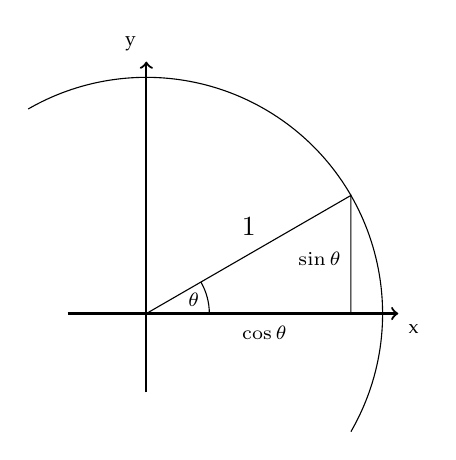
\begin{tikzpicture}
        \draw[thick,->] (-1,0) -- (3.2,0) node[anchor=north west] {\scriptsize x};
        \draw[thick,->] (0,-1) -- (0,3.2) node[anchor=south east] {\scriptsize y};
        \draw (2.598,-1.5) arc (-30:120:3);       
        \draw (0,0) -- (2.598,0) -- (2.598,1.5) -- cycle;
        \node at (1.5,-0.25) {\scriptsize $\cos \theta$};
        \node at (2.2,0.7) {\scriptsize $\sin \theta$};
        \node at (1.3,1.1) {$1$};
        \node at (0.6,0.17) {\scriptsize $\theta$};
        \draw (0.8,0) arc(0:30:0.8);
    \end{tikzpicture}
    \caption{The unit circle} \label{fig:unit-circle}
\end{figure}

The points that make up the circumference (edge) of a unit circle are all the points that are $1$ unit of distance from the centre. The same definition is used for a sphere in any number of spatial dimensions.

For historical reasons\footnote{The ratio between the diameter, $d$ of a circle and the circumference is $\pi$. But it has turned out over succeeding millennia that the radius $r = d/2$ is far more commonly encountered in calculations, and so we are doomed to say $2\pi$ almost everywhere.} when measuring distances travelled around the circumference of a unit circle we define the number $\pi$ to be the length of half a circumference, so length of the circumference of a unit circle is $2\pi$. We call this distance travelled around a part of the unit circle's circumference the \textit{angle}. By convention we always begin measuring the angle from the $x$-axis and moving in the counter-clockwise direction. In the figure the angle $\theta$ happens to be $\pi/6$, the same as 30$^\circ$.

\section{Sine and Cosine}

Given an angle, it is surely possible to compute the $(x, y)$ coordinates of the corresponding point on the circumference. There must exist a pair of functions that give these coordinates, traditionally named as follows:

\begin{itemize}
    \item $\sin \theta$ ("sine") gives the vertical or $y$ coordinate, and
    \item $\cos \theta$ ("cosine") gives the horizontal or $x$ coordinate.
\end{itemize}

Without knowing anything else about these functions, we can already see that as an object progresses around the circle, its coordinates must visit these milestones:

\begin{itemize}
    \item We begin at $\theta = 0$, the right-most point of the circle, where $\sin \theta = 0$ and $\cos \theta = 1$.
    \item At $\theta = \pi/2$ (90$^\circ$), the top of the circle, the situation has reversed: $\sin \theta = 1$ and $\cos \theta = 0$.
    \item At $\theta = \pi$ (180$^\circ$), the left-most point of the circle, $\sin \theta = 0$ and $\cos \theta = -1$.
    \item At $\theta = 3\pi/2$ (270$^\circ$), the bottom of the circle, $\sin \theta = -1$ and $\cos \theta = 0$.
\end{itemize}

We can plot $\sin \theta$ by itself (Figure \ref{fig:sin}) between the values $0$ and $2\pi$, and likewise $\cos \theta$ (Figure \ref{fig:cos}).

\begin{figure}[h]
    \caption{Sine and Cosine}
    \begin{subfigure}{0.5\textwidth}
        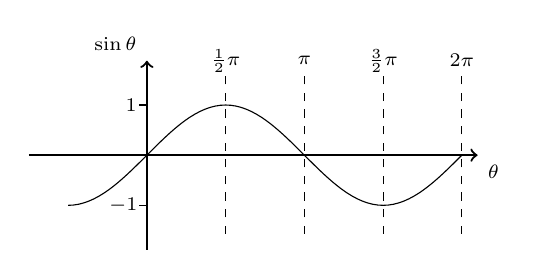
\begin{tikzpicture}
            \draw[thick,->] (-0.5,0) -- (5.2,0) node[anchor=north west] {\scriptsize $\theta$};
            \draw[thick,->] (1,-1.2) -- (1,1.2) node[anchor=south east] {\scriptsize $\sin \theta$};
            \draw (0,-0.637) cos(1,0) sin (2,0.637) cos (3,0) sin (4,-0.637) cos (5,0);
            \draw[dashed] (2,-1) -- (2,1);
            \draw[dashed] (3,-1) -- (3,1);
            \draw[dashed] (4,-1) -- (4,1);
            \draw[dashed] (5,-1) -- (5,1);
            \node at (2,1.2) {\scriptsize $\frac{1}{2}\pi$};            
            \node at (3,1.2) {\scriptsize $\pi$};            
            \node at (4,1.2) {\scriptsize $\frac{3}{2}\pi$};
            \node at (5,1.2) {\scriptsize $2\pi$};
            \draw (0.9,0.637) -- (1,0.637);
            \node at (0.8,0.637) {\scriptsize $1$};
            \draw (0.9,-0.637) -- (1,-0.637);
            \node at (0.7,-0.637) {\scriptsize $-1$};
        \end{tikzpicture}
    \caption{The $\sin$ function} \label{fig:sin}
    \end{subfigure}
    \begin{subfigure}{0.5\textwidth}
        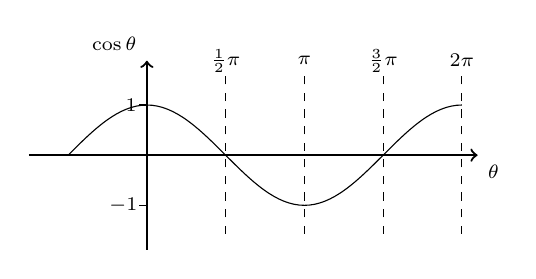
\begin{tikzpicture}
            \draw[thick,->] (-0.5,0) -- (5.2,0) node[anchor=north west] {\scriptsize $\theta$};
            \draw[thick,->] (1,-1.2) -- (1,1.2) node[anchor=south east] {\scriptsize $\cos \theta$};
            \draw (0,0) sin (1,0.637) cos (2,0) sin (3,-0.637) cos (4,0) sin(5, 0.637);
            \draw[dashed] (2,-1) -- (2,1);
            \draw[dashed] (3,-1) -- (3,1);
            \draw[dashed] (4,-1) -- (4,1);
            \draw[dashed] (5,-1) -- (5,1);
            \node at (2,1.2) {\scriptsize $\frac{1}{2}\pi$};            
            \node at (3,1.2) {\scriptsize $\pi$};            
            \node at (4,1.2) {\scriptsize $\frac{3}{2}\pi$};
            \node at (5,1.2) {\scriptsize $2\pi$};
            \draw (0.9,0.637) -- (1,0.637);
            \node at (0.8,0.637) {\scriptsize $1$};
            \draw (0.9,-0.637) -- (1,-0.637);
            \node at (0.7,-0.637) {\scriptsize $-1$};
        \end{tikzpicture}
        \caption{The $\cos$ function} \label{fig:cos}
    \end{subfigure}
\end{figure}

We can see that $\cos$ is just $\sin$ advanced by a quarter of a cycle, or:

$$
\cos \theta = \sin (\theta + \pi/2)
$$ 

If we advanced $\sin$ by $\pi$, half a cycle, the peaks and valleys would change places, while the uphill slopes that cut through the horizontal axix would become downhill slopes and vice versa. In other words, it would look exactly like we'd flipped the $\sin$ function upside down:

\begin{figure}[h]
    \centering
    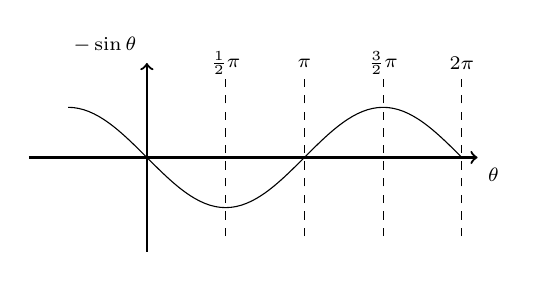
\begin{tikzpicture}
        \draw[thick,->] (-0.5,0) -- (5.2,0) node[anchor=north west] {\scriptsize $\theta$};
        \draw[thick,->] (1,-1.2) -- (1,1.2) node[anchor=south east] {\scriptsize $-\sin \theta$};
        \draw (0,0.637) cos(1,0) sin (2,-0.637) cos (3,0) sin (4,0.637) cos (5,0);
        \draw[dashed] (2,-1) -- (2,1);
        \draw[dashed] (3,-1) -- (3,1);
        \draw[dashed] (4,-1) -- (4,1);
        \draw[dashed] (5,-1) -- (5,1);
        \node at (2,1.2) {\scriptsize $\frac{1}{2}\pi$};            
        \node at (3,1.2) {\scriptsize $\pi$};            
        \node at (4,1.2) {\scriptsize $\frac{3}{2}\pi$};
        \node at (5,1.2) {\scriptsize $2\pi$};        
    \end{tikzpicture}
    \caption{$\sin \theta$ upside down} \label{fig:minus-sin}
\end{figure}

So:

$$
-\sin \theta = \cos (\theta + \pi/2) = \sin (\theta + \pi)
$$

Incidentally, the word \textit{cycle} is from the Greek word for circle. The word \textit{phase} is also used a lot in this context, probably deriving from the phases of the moon. When one periodic function is equal to another shifted by some amount, we say there is only a phase difference between them.

\section{Differential Calculus on Sine and Cosine}

Think of an object moving along the unit circle's edge at a constant rate. It has an instantaneous velocity vector pointing along the tangent, but this is always at a right angle to the line segment reaching from the centre to the object (the radius).

\begin{figure}[h]
    \centering
    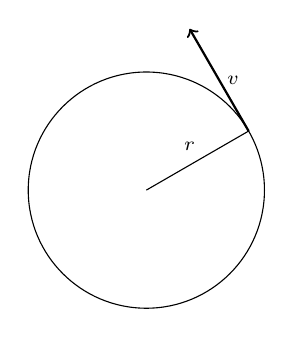
\begin{tikzpicture}
        \draw (0,0) circle(1.5);
        \draw (0,0) -- (1.299,0.75);
        \draw[thick,->] (1.299,0.75) -- (0.549,2.049);
        \node at (0.55,0.55) {\scriptsize $r$};
        \node at (1.1,1.4) {\scriptsize $v$};
            
    \end{tikzpicture}
    \caption{The velocity vector $v$ of an orbiting object} \label{fig:circle-tangent}
\end{figure}

The velocity vector is therefore fixed to be a quarter cycle ahead of the radius, which is precisely the relationship between $\cos \theta$ and $\sin \theta$. The components of $v$ are the rates at which the corresponding components of $r$ change as the angle advances. It follows that the rate at which $\sin \theta$ is increasing is given by $\cos \theta$, or:

$$
\frac{d}{d\theta} \sin \theta = \cos \theta
$$

This is confirmed by examining the shape of the functions separately. Nearby to $\theta = 0$, $\sin \theta$ is closely approximated by $\theta$ itself, and looks (Figure \ref{fig:sin-small}) much like a straight line of gradient $1$, which happens to be the value of $\cos 0$.

\begin{figure}[h]    
    \caption{Gradients of Sine}
    \begin{subfigure}{0.5\textwidth}
        \centering
        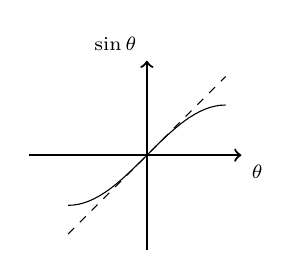
\begin{tikzpicture}
            \draw[thick,->] (-0.5,0) -- (2.2,0) node[anchor=north west] {\scriptsize $\theta$};
            \draw[thick,->] (1,-1.2) -- (1,1.2) node[anchor=south east] {\scriptsize $\sin \theta$};
            \draw (0,-0.637) cos(1,0) sin (2,0.637);
            \draw[dashed] (0,-1) -- (2,1);
        \end{tikzpicture}
    \caption{$\sin \theta \approx \theta$} \label{fig:sin-small}
    \end{subfigure}
    \begin{subfigure}{0.5\textwidth}
        \centering
        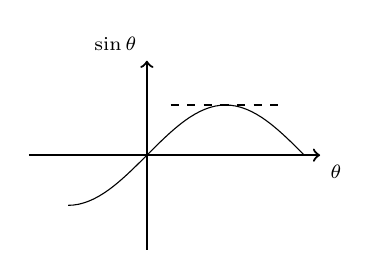
\begin{tikzpicture}
            \draw[thick,->] (-0.5,0) -- (3.2,0) node[anchor=north west] {\scriptsize $\theta$};
            \draw[thick,->] (1,-1.2) -- (1,1.2) node[anchor=south east] {\scriptsize $\sin \theta$};
            \draw (0,-0.637) cos(1,0) sin (2,0.637) cos (3,0);
            \draw[dashed] (1.3,0.637) -- (2.7,0.637);
        \end{tikzpicture}
        \caption{Gradient $0$} \label{fig:sin-peak}
    \end{subfigure}
\end{figure}

When $\sin \theta$ peaks at $\theta = \pi/2$, its gradient is $0$, and again this is in agreement with the value of $\cos (\pi/2)$. This pattern continues at every point in the cycle.

So in any situation where we need the derivative of $\sin$, we just replace it with $\cos$. By the same reasoning (and because we know the same relationship exists between $-\sin \theta$ and $\cos \theta$) we can assume that:
$$
\frac{d}{d\theta} \cos \theta = -\sin \theta
$$

Differentiating two more times will get us back to $\sin \theta$ because each differentiation advances the function by a quarter cycle. Naturally integration performs the same trick in the opposite direction.

\section{Computing Sine and Cosine} \label{sec:unit-circle-maclaurin}

Now we can take the derivative of $\sin$, and we know its precise value at $0$ (and those of its derivatives), we can use the Maclaurin method to find how to compute it using only addition and multiplication, if only we have the patience to perform an infinite sequence of those operations. We begin by assuming that a function $f(x)$ can be expressed as the sum of an infinite series of polynomial terms, that is, some constant $a_n$ multiplied by the variable $x$ raised to an integer power $n$, beginning at $0$:

$$
f(x) = a_0x^0 + a_1x^1 + a_2x^2 + a_3x^3 + \ldots
$$

Anything raised to the power of $0$ is $1$, and raising something to the power of $1$ makes no difference, so at the expense of consistency, and meanwhile also naming the function we want to compute, we just write:

$$
\sin x = a_0 + a_1x + a_2x^2 + a_3x^3 + \ldots
$$

So we only need to determine the constant factors $a_n$ to entirely characterise the function. Setting $x = 0$, any term that is multiplied by $x$ must be zero (they \textit{vanish} entirely from the sum), which only leaves $a_0$. But $\sin 0 = 0$, so it follows that $a_0 = 0$. Taking the derivative of both sides:

$$
\cos x = a_1 + 2a_2x + 3a_3x^2 + 4a_4x^3 + \ldots
$$

Each polynomial's power is reduced by $1$, and the original power "moves down" to become an extra factor. Now the exact same vanishing argument applies to $a_1$ except that here it is solely responsible for the value of $\cos 0 = 1$, and so it must be that $a_1 = 1$. We differentiate a second time:

$$
-\sin x = 2a_2 + (3\cdot2)a_3x + (4\cdot3)a_4x^2 + \ldots
$$

So $a_2 = 0$. Differentiate a third time:

$$
-\cos x = (3\cdot2)a_3 + (4\cdot3\cdot2)a_4x + \ldots
$$

So $a_3 = -\frac{1}{3!}$. When $n$ is even the term is zero, and when $n$ is odd the term $x^n$ is divided by the accumulated value $n!$. We continue in this fashion to find that:

$$
\sin x = x - \frac{x^3}{3!} + \frac{x^5}{5!} - \frac{x^7}{7!} + \frac{x^9}{9!} - \ldots
$$

By the same process we find that for $cos$ only the even-$n$ terms appear in the result:

$$
\cos x = 1 - \frac{x^2}{2!} + \frac{x^4}{4!} - \frac{x^6}{6!} + \frac{x^8}{8!} - \ldots
$$

In each case there is a four stage cycle, with alternating absence of terms and then similarly alternating $+$/$-$ signs. This is curiously reminiscent of the cyclic behaviour of imaginary unit number $i$, defined such that $i^2 = -1$, as we raise it to integer powers starting at zero:

\begin{itemize}
    \item $i^0 = 1$
    \item $i^1 = i$
    \item $i^2 = -1$
    \item $i^3 = i(i^2) = -i$
    \item $i^4 = (i^2)(i^2) = (-1)(-1) = 1$
    \item and so on: $i$, $-1$, $-i$, $1$, $i$, $-1$ $\ldots$
\end{itemize}

\section{Euler's Formula}

If we get carried away by the power of this method we risk drifting from the topic of the unit circle, but it turns out that there is no escape.

The exponential function $e^x$ raises the constant $e$ to a variable power, and the value $e$ is chosen such that the derivative is $e^x$, so the function is its own derivative. The method of evaluating at zero and taking repeated derivatives is therefore particularly simple to perform and yields:

$$
e^x = 1 + x + \frac{x^2}{2!} + \frac{x^3}{3!} + \frac{x^4}{4!} + \frac{x^5}{5!} + \ldots
$$

This is obviously different from the previous two examples because no terms vanish and all terms are positive. But what happens if we replace $x$ with $xi$?

$$
e^{ix} = 1 + ix + \frac{i^2x^2}{2!} + \frac{i^3x^3}{3!} + \frac{i^4x^4}{4!} + \frac{i^5x^5}{5!} + \ldots
$$

Simplifying the various powers of $i$ according to its definition:

$$
e^{ix} = 1 + ix - \frac{x^2}{2!} - i\frac{x^3}{3!} + \frac{x^4}{4!} + i\frac{x^5}{5!} + \ldots
$$

It appears we can write it as the sum of two series, one containing only real terms and the other only imaginary:

$$
e^{ix} = (1 - \frac{x^2}{2!} + \frac{x^4}{4!} - \ldots) + i(x - \frac{x^3}{3!} + \frac{x^5}{5!} - \ldots)
$$

But the real component is evidently $\cos x$ while the imaginary one is $\sin x$!

$$
e^{ix} = \cos x + i\sin x
$$

This means that $x$ is the angle, so we will resuming calling it $\theta$. We can interpret $e^{i\theta}$ as a unit circle in the complex plane. It is all the complex numbers of modulus 1.

We can relabel the axes on our diagram of the unit circle, to show the circle in the complex plane (Figure \ref{fig:unit-circle-complex}).

\begin{figure}[h]
    \centering
    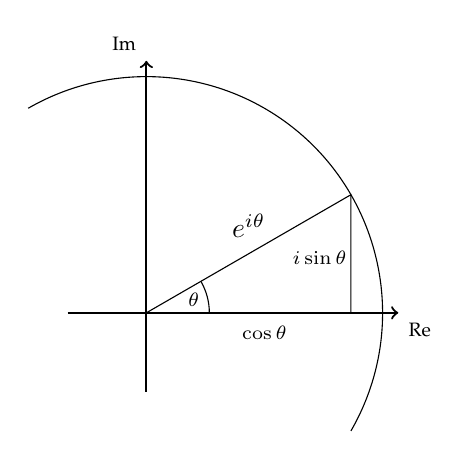
\begin{tikzpicture}
        \draw[thick,->] (-1,0) -- (3.2,0) node[anchor=north west] {\scriptsize Re};
        \draw[thick,->] (0,-1) -- (0,3.2) node[anchor=south east] {\scriptsize Im};
        \draw (2.598,-1.5) arc (-30:120:3);
        \draw (0,0) -- (2.598,0) -- (2.598,1.5) -- cycle;
        \node at (1.5,-0.25) {\scriptsize $\cos \theta$};
        \node at (2.2,0.7) {\scriptsize $i\sin \theta$};
        \node at (1.3,1.1) {$e^{i\theta}$};
        \node at (0.6,0.17) {\scriptsize $\theta$};
        \draw (0.8,0) arc(0:30:0.8);
    \end{tikzpicture}
    \caption{The unit circle in the complex plane} \label{fig:unit-circle-complex}
\end{figure}

We can scale the circle to any radius $r$ simply by multiplying by that radius. This means we can represent any complex number either as a sum $x + yi$, or as an exponential $re^{i\theta}$.

Physics is thick with examples of oscillation. To describe the state of a particle undergoing simple harmonic motion along a line, we need to know the position and the momentum. But a complex number, being described by two real numbers, can encapsulate both these quantities, and the real and imaginary parts have the right phase relationship.

\section{Pythagoras in the Circle}

There is a right-triangle in the diagram, so by Pythagoras:

$$
x^2 + y^2 = 1
$$

it must be that:

$$
(\sin \theta)^2 + (\cos \theta)^2 = 1
$$

Also by Pythagoras, given one coordinate of a point on the circle, we can compute the other:

\begin{center}
    $y = \sqrt{1 - x^2}$ \quad $x = \sqrt{1 - y^2}$    
\end{center}

\chapter{From Vectors to Tensors} \label{ch:vectors}

\section{What we need to unlearn}

We are first introduced to vectors in two different yet closely related and simplified forms. We're now going to rethink them as an abstraction, which will require us to be careful not to depend on any intuitions derived from our earlier encounters.

That's not to say that we will be abandoning the schoolhouse version of vectors; rather, we will be properly placing them in the context of a more general framework. Also they will very often help ground us, as long as we recognise their limitations.

\subsection{Arrows with direction and length}

The first way to think of vectors is by visualising them as arrows that have a direction and a length. Two vectors $\vec{a}$ and $\vec{b}$ can be added (Figure \ref{fig:vector-addition}) by laying them head to tail, so the sum $\vec{c}$ is the vector starting at the tail of $\vec{a}$ and ending at the head of $\vec{b}$.

\begin{figure}[h]
    \centering
    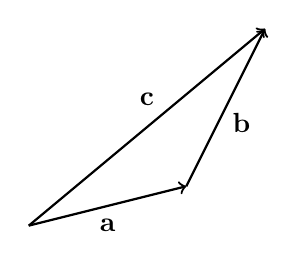
\begin{tikzpicture}        
        \draw[thick,->] (0,0) -- (2,0.5);
        \node at (1,0) {$\vec{a}$};
        \draw[thick,->] (2,0.5) -- (3,2.5);
        \node at (2.7,1.3) {$\vec{b}$};
        \draw[thick,->] (0,0) -- (3,2.5);
        \node at (1.5,1.6) {$\vec{c}$};
    \end{tikzpicture}
    \caption{Adding arrows.} \label{fig:vector-addition}
\end{figure}

Scaling a vector (multiplying it by a number) just alters its length without changing its direction, e.g. multiply by $0.5$ to shrink the vector to half its prior length.

We also learn about the dot product, a scalar-valued operator between two vectors, $\vec{p}\cdot\vec{q}$. If the two vectors $\vec{p}$ and $\vec{q}$ are separated by angle $\theta$, and we know the magnitude (length) of each vector, e.g. $\|\vec{p}\|$, then:

$$
\vec{p}\cdot\vec{q} = \|\vec{p}\| \|\vec{q}\|\cos{\theta}
$$

When we get onto the abstract definition of a vector it may seem like the geometric viewpoint has been relegated to a special case, less fundamental. But it is often useful to keep it in your mind as a way to visualise vectors of any kind, because however abstractly they are defined, they will always be closely analogous to the familiar arrows.

\subsection{Columns of numbers}

The second concrete way to think of vectors is as columns of ordinary numbers, and the number of \textit{dimensions} of the space tells us how many numbers a column vector has to contain. In this form, to add two vectors we just deal with the rows separately: add the numbers in row $1$, and then the numbers in row $2$ and so on for however many rows there are in a column vector, and thus obtain the sum as a column:

$$
\begin{bmatrix}2 \\ 0.5\end{bmatrix} +
\begin{bmatrix}1 \\ 2\end{bmatrix} =
\begin{bmatrix}3 \\ 2.5\end{bmatrix}
$$

More succinctly we can use index notation $a_n$ to mean the value in the $n$th row of the column associated with vector $\vec{a}$, so to add two vectors we just do this:

$$
a_n + b_n = c_n
$$

Scaling a vector just involves multiplying all the rows by the same number:

$$
d_n = x a_n
$$

The dot product is extremely simple in this representation: like with addition, you treat each row separately, multiplying the numbers in row $1$ and so on, but then you just sum all the products to get the numeric value:

$$
\sum_n a_n b_n
$$

\subsection{Coordinates}

These two perspectives are united by introducing a coordinate grid (Figure \ref{fig:vector-coordinate-grid}).

\begin{figure}[h]
    \centering
    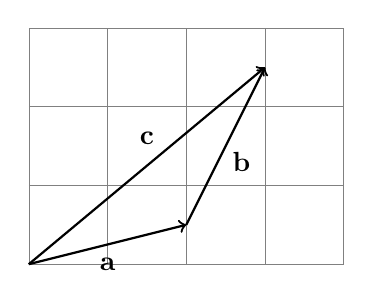
\begin{tikzpicture}       
        \draw[step=1cm,gray,very thin] (0,0) grid (4,3); 
        \draw[thick,->] (0,0) -- (2,0.5);
        \node at (1,0) {$\vec{a}$};
        \draw[thick,->] (2,0.5) -- (3,2.5);
        \node at (2.7,1.3) {$\vec{b}$};
        \draw[thick,->] (0,0) -- (3,2.5);
        \node at (1.5,1.6) {$\vec{c}$};
    \end{tikzpicture}
    \caption{Coordinate grid.} \label{fig:vector-coordinate-grid}
\end{figure}

Much of this subject is concerned with ensuring that our choice of coordinate grid doesn't get confused with the physical facts. We're trying to get answers about nature, and those answers better not change just because we used a different coordinate grid. One of the most important ideas in physics is that vectors are primarily geometric objects. They can be described with numeric coordinates, but there is no preferred coordinate basis. A vector has an independent existence, because it describes something in the physical world.

But however abstract things get, it can often be helpful to remember that you can visualise vectors as arrows and think of the basic operations on them geometrically, and equally it can be helpful to remember that we will always have a way of representing vectors as columns of numbers (indeed, columns of numbers \textit{are} vectors.)

The primary intuition we've been implicitly relying on so far is \textit{orthonormality}. With arrow vectors we can simply see when they are orthogonal, or to be more precise we can measure the angle between vectors, and we can measure their lengths, and we can choose a unit length, and so on. We can simply draw a unit vector, and then draw another unit vector that is orthogonal to it.

Likewise from the column vectors we have no difficult choosing a set of orthonormal vectors, the \textit{standard basis}. They are \textit{one-hot}, all values zero except for a single $1$. In an $n$-dimensional space there can only be $n$ such distinct vectors.

None of these intuitive leaps will be available with abstract vector spaces, and orthonormality cannot be used as an elemental building block. We will build a quite rich set of more fundamental concepts before we invent orthonormality.

By the way, when in physics we speak of a \textit{vector field}, that is, a vector at each point in space, such as wind speed and direction, or the electric field, we visualise arrows spread out over space. But the value of the field in two different places may be the same.

This is obvious (and less confusing) in the case of a scalar field, such as temperature. At two different locations in a room, the temperature may be the same. It's a numerical value that varies from place to place, and the same number may appear in two places.

But exactly the same is true for a vector field. If the wind is some particular speed and direction at two different places on the map, we say the vectors are equal: they are the \textit{same vector}. From the point of view of considering their equality, it is irrelevant that they are associated with different locations in physical space. In vector space, there is one vector with that direction and length.

On to the abstract stuff.

\section{Vectors as elements of a vector space}\label{sec:vectors-space}

A vector space is a set of objects, called vectors, about which we assume nothing except that we can perform certain operations on them.

\subsection{They can be added}

There is an operator $+$ that takes two objects from the set and returns another from the same set (we say it's a \textit{closed} operator).

This operator is commutative:

$$\vec{u} + \vec{v} = \vec{v} + \vec{u}$$

and associative:

$$\vec{u} + (\vec{v} + \vec{w}) = (\vec{v} + \vec{u}) + \vec{w}$$

There is a special object called $0$ (the \textit{zero vector}), which makes no difference when added to any object from the set:

$$\vec{v} + 0 = \vec{v}$$

Also every object has an opposite, known as its additive inverse, so they pair up. The inverse of $\vec{v}$ is written as $-\vec{v}$, and:

$$\vec{v} + (-\vec{v}) = 0$$

The above can written as $\vec{v} - \vec{v}$. Evidently $0$ is its own inverse.

Referring back to schoolhouse vectors, we can see how the arrows and the columns have an addition operation that satisfies all these requirements.

\subsection{They can be scaled}

There is an associated set of objects called scalars, typically restricted to real or complex numbers. Our objects can be multiplied by a scalar to get another object. Scaling them by $1$ makes no difference. Scaling them by $-1$ discovers the additive inverse.

Given two scalars $a$ and $b$, we can compute $c = ab$ and then scale an object $\vec{v}$ by it, or we can separately scale the object first by $a$ and then by $b$, and the result is the same:

$$(ab)\vec{v} = a(b\vec{v})$$

Scaling is distributive over addition of objects:

$$a(\vec{u} + \vec{v}) = a\vec{u} + a\vec{v}$$

And also over addition of scalars:

$$(a + b)\vec{v} = a\vec{v} + b\vec{v}$$

Again, arrows and columns have no problem meeting these requirements.

\subsection{Other Examples of Vector Spaces}

Any set of objects for which we can define these operations is a vector space, not just arrows and columns. The set of ordered tuples of real numbers $\mathbb{R}^n$ is just the column vectors with $n$ rows each. Also there is no reason why $n$ shouldn't be $1$, which means that the plain old set of real numbers $\mathbb{R}$ is also vector space. Think of the real number line as My First Vector Space\texttrademark.

Also the complex numbers $\mathbb{C}$, and tuples of them $\mathbb{C}^n$, work just as well. The example of $\mathbb{C}$ as a vector space is particularly interesting because of its close similarly to $\mathbb{R}^2$. The major difference is that it has a definition of multiplication as a closed operation over its vectors (such that the product of two vectors is a vector), which is absolutely not a general feature of vector spaces.\footnote{Although it is also defined (very differently) in $\mathbb{R}^3$ as the cross product, $\times$.}

In quantum mechanics we will contend with infinite-dimensional complex vector spaces.

\subsection{Fields}

The kind of set that can serve as a scalar is called by mathematicians a \textit{field} (an unfortunate collision of terminology given the very different meaning in physics), which is a set of objects on which we have defined addition, subtraction, multiplication and division, so real or complex numbers usually serve this purpose (and always do in physics), but vectors in general cannot serve as a field of scalars for other vector spaces, because the definition of a vector space says nothing about there being a natural way to multiply or divide pairs of vectors to obtain other vectors.

In the same way, you can't have a vector space of $\mathbb{R}$ over the field of $\mathbb{C}$, because although we can use regular multiplication to "scale" a vector from $\mathbb{R}$ by a scalar from $\mathbb{C}$, the result is likely to be a member of $\mathbb{C}$ but not of $\mathbb{R}$, and thus not a vector from the same space.

Unless we say otherwise, we'll assume the field is $\mathbb{R}$.

\subsection{Finding a Basis}

If we select two vectors $\vec{a}$ and $\vec{b}$ from the space, we may find that they only differ by a scalar ratio $x$:

$$
\vec{a} = x \vec{b}
$$

If there is an $x$ that can scale $\vec{b}$ into $\vec{a}$ then those two vector are \textit{colinear}\footnote{This literally means "on the same line". Note the interesting use of geometrical language, even though we're not supposed to be thinking about arrows in this abstract discussion} (we are careful not to say they point in the same direction because if $x$ is negative then they point in exactly opposite directions, but are still colinear.)

But if there is no such $x$ then they are not colinear. This gives them an interesting superpower:

$$
\vec{r} = x \vec{a} + y \vec{b}
$$

By varying the scalar coefficients $x$ and $y$ we can construct any vector $\vec{r}$ in a two-dimensional \textit{subspace} of the vector space.

We can generalise on this idea a bit by rearranging the equation (and supposing that $x$ becomes negative). If for two vectors $\vec{a}$ and $\vec{b}$ we can find a scalar ${x}$ so that:

$$ 
\vec{a} + x \vec{b} = 0
$$

then they are colinear. Suppose the two vectors point in the same direction but $\vec{a}$ is twice the length of $\vec{b}$. Then we can set $x = -2$ and the sum will cancel out. This is only possible because they are colinear. If it's not possible, we've found a pair of \textit{linearly independent} vectors. Now we can look for a third:

$$ 
\vec{a} + x \vec{b} + y \vec{c} \ne 0
$$

Supposing we find such a vector $\vec{c}$ for which there is no scalar $y$ that satisfies the above equation, then we have found three linearly independent vectors. Or to put it another way, it is not possible to make $\vec{c}$ by any weighted sum of $\vec{a}$ and $\vec{b}$:

$$
\vec{c} \ne x \vec{a} + y \vec{b}
$$

Now we can construct any vector in three dimensions:

$$
\vec{r} = x \vec{a} + y \vec{b} + z \vec{c}
$$

Eventually we may find (assuming the space is finite dimensional) that it is not possible to extend our linearly independent set $\vec{a}, \vec{b}, \vec{c}, ...$ any further. The size of this set tells us how many dimensions the space has, and these vectors are said to \textit{span} the space.

The vitally important thing to realise about this is that at no point have we said that these vectors are orthogonal. We haven't even defined what that means yet. We've only defined the property of linear independence. Nevertheless we have arrived at the idea of a coordinate grid; it's just that our grid may be awkwardly slanted, made of identical parallelogram tiles rather than identical square tiles.

So we don't have to keep choosing letters, we will label each dimension with a number. The set of linearly independent vectors that we can use to construct any other vector in the space is called a \textit{basis}. The basis vectors are traditionally written as $\vec{e}_n$, where $n$ is often 1-based (although in Relativity it is usually 0-based). The scalar coefficients, which we will call coordinates, that construct a given vector $\vec{r}$ can also be numbered, conventionally with superscript $r^n$:

\begin{equation}
\begin{split}
\vec{r} &= r^1 \vec{e}_1 + r^2 \vec{e}_2 + ... + r^n \vec{e}_n \\
        &= \sum_n r^n \vec{e}_n
\end{split}
\end{equation}

The use of a superscript index is obviously asking for trouble given that it looks like we're raising $r$ to a power, but this notation is universal in physics so we may as well get used to it.

Having chosen a basis, we can describe any vector with a tuple of coordinates $r^n$, so any vector space of dimension $N$ whose scalar field is $\mathbb{F}$ must be isomorphic with $\mathbb{F}^N$. In other words, all vectors can be described by column vectors, but the numbers in the columns will depend on our choice of basis.

But the laws of physics cannot possibly care what basis we choose, so we need ways of obtaining numeric facts about vectors that do not depend on the choice of basis.

\section{Covectors}

Think of a scalar-valued function of a vector. That is, a black box with a single input slot accepting a vector $\vec{a}$, and an output hole that gives us back a scalar $x$ (Figure \ref{fig:1-slot-box}).

\begin{figure}[h]
    \centering
    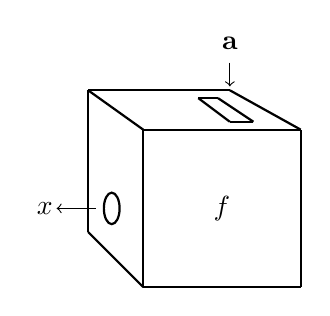
\begin{tikzpicture}
        \draw[thick] (0,0) -- (2,0);
        \draw[thick] (2,0) -- (2,2);
        \draw[thick] (2,2) -- (0,2);
        \draw[thick] (0,2) -- (0,0);
        \draw[thick] (0,2) -- (-0.7,2.5);
        \draw[thick] (-0.7,2.5) -- (-0.7,0.7);
        \draw[thick] (-0.7,0.7) -- (0,0);
        \draw[thick] (-0.7,2.5) -- (1.1,2.5);
        \draw[thick] (1.1,2.5) -- (2,2);

        \draw[thick] (1.4,2.1) -- (0.95,2.4);
        \draw[thick] (0.95,2.4) -- (0.7,2.4);
        \draw[thick] (0.7,2.4) -- (1.1,2.1);
        \draw[thick] (1.1,2.1) -- (1.4,2.1);
        
        \node at (1.1,3.1) { $\vec{a}$};
        \draw[->] (1.1,2.85) -- (1.1,2.55);

        \node at (-1.25,1) { $x$};
        \draw[thick] (-0.4,1) ellipse (0.1 and 0.2);
        \draw[->] (-0.6,1) -- (-1.1,1);

        \node at (1,1) { $f$};

    \end{tikzpicture}
    \caption{Function $f$ with a single slot accepting a vector} \label{fig:1-slot-box}
\end{figure}

More precisely, this machine is a mapping from the vector space to the real numbers. There are infinitely many such mappings and they could be rather complicated. We will restrict ourselves to a simple subset of these mappings.

First, we note that it is possible to define the addition operator on mappings:

$$
f(\vec{a}) = g(\vec{a}) + h(\vec{a})
$$

That is, it could be that inside the box $f$, there are concealed two boxes $g$ and $h$. When $f$ receives an input vector $\vec{a}$, it passes it to both $g$ and $h$, and adds their results together to obtain its own result. Note that we haven't yet restricted the complexity of $g$ and $h$; we have no idea what they do to produce their individual results.

Likewise, it is possible to scale a mapping by a factor $x$:

$$
f(\vec{a}) = x g(\vec{a})
$$

The trick to restricting the complexity of our set of possible mappings is to require that they comply with the rules of a vector space. Not only can they be added and scaled, but combinations of these operations produce consistent results. But if we do that, then we have also ensured that the set of allowed mappings actually \textit{is} a vector space. Every mapping we care about must be a vector chosen from that space.

Note that we haven't proven that every possible mapping is a vector. We've merely restricted ourselves to only considering a subset of mappings, those that can be scaled and added to find other mappings from the same restricted subset, such that scaling a mapping by 5 is the same as scaling that mapping by 2 and separately by 3 and then adding those two scaled mappings.

If we label the original vector space $V$ then this associated vector space of mappings $V \mapsto \mathbb{R}$ is written as $V^*$ and is called the dual space of $V$. All we've discovered so far about $V$ also applies to $V^*$, including the idea of a set of mappings being linearly independent, which means we can select a basis of mappings chosen from $V^*$ and thus construct any mapping from it by scaling and adding the basis mappings. That's quite a leap, so pause to digest it. The moment you discover a set of objects is a vector space, you know you can choose a basis, and then describe anything in that space in terms of a weighted sum of that basis.

We call the mappings taken from $V^*$ \textit{covectors}. The basis covectors are labelled with superscripts $\vec{e}^n$ and the coordinates with subscripts $f_n$, so we can build any covector from the chosen basis:

\begin{equation}
    \begin{split}
    \vec{f} &= f_1 \vec{e}^1 + f_2 \vec{e}^2 + ... + f_n \vec{e}^n \\
            &= \sum_n f_n \vec{e}^n
    \end{split}
\end{equation}

It follows that, just as $N$-dimensional vectors are isomorphic with columns of $N$ scalars, so too are their associated covectors.

It is sometimes suggested that all vector spaces have a dual space, as if this was some property hiding in the definition of a vector space. But in truth we have conjured the dual space into existence, first by inventing the idea of a mapping $V \mapsto \mathbb{R}$, then by defining operations on those mappings, then by considering the set of all possible mappings, and finally by imposing the rules of vector spaces, which restricts us to a subset of the possible mappings that we named covectors. There is nothing particularly automatic about this. We made it happen by being curious about ways in which vectors might be mapped to scalars.

Another important point to note is that as covectors are vectors, the operation we've been writing as $f(\vec{a})$ is in fact much more symmetrical than that notation implies. We combine a vector from $V$ and a covector from $V^*$ and this produces a scalar from $\mathbb{R}$. 

So we could equally say that a vector "operates" on a covector to produce the scalar. From the point of view of $V^*$ it is $V$ that is the dual space. There is a more symmetrical notation\footnote{Unfortunately there is almost no consistency on notation in this topic; we're just picking one of many possible notations for this.} we can use to make this clear:

$$\langle \vec{f},\vec{a}\rangle$$

In this notation, the left and right sides of the operation are from mutually dual spaces, mirror opposites that annihilate one another leaving only a scalar residue.

Keep in mind that just as we've thought of a covector as machine that accepts a vector as input, we could just as well think of a vector as a machine that accepts a covector as input.

\subsection{Connecting the Dual Spaces}

We obviously have a lot of freedom when choosing a basis in either $V$ or $V^*$. What can we usefully do to relate the two sides? We've seen how a covector is built as a weighted sum of basis covectors $\vec{e}^i$ from $V^*$:

$$
\vec{f} = \sum_i f_i \vec{e}^i
$$

And likewise a vector is built as a weighted sum of basis vectors $\vec{e}_i$ from $V$:

$$
\vec{v} = \sum_i v^i \vec{e}_i
$$

If we have the vector $\vec{v}$ and we want to extract its $i$th coordinate, $v^i$, that's a function from a vector in $V$ to a scalar, that is, it's a covector from $V^*$. We could choose the basis covectors so that the $i$th basis covector extracts the $i$th coordinate of the vector passed to it:

$$
v^i = \langle \vec{e}^i , \vec{v} \rangle
$$ 

Equivalently, if we have a covector $\vec{f}$ and we want to extract its $j$th coordinate, $f_j$, then we need to pass $f$ an input vector chosen from $V$, and we could choose the basis vectors so that the $j$th basis vector makes $\vec{f}$ produce the $j$th coordinate of $\vec{f}$:

$$
f_j = \langle \vec{f} , \vec{e}_j\rangle
$$

It doesn't matter which of those two ways we approach this, because either will constrain the other. We can substitute $\vec{f}$ expressed as a sum:

$$
f_j = \langle \sum_i f_i \vec{e}^i , \vec{e}_j\rangle
$$

and linearity allows us to separately deal with each dimension and sum their results:

$$
f_j = \sum_i f_i \langle \vec{e}^i , \vec{e}_j\rangle
$$

But if that's true for \textit{any} $\vec{f}$, and not just a coincidence applying to some specific example, then the scalar factor $\langle \vec{e}^i , \vec{e}_j\rangle$ must be "selecting" just one of the $f_i$ terms, specifically the one where $i = j$, and eliminating all others, or to put it another way:

$$
f_j = \sum_i f_i \delta \indices{^i_j}
$$

So if the $f_j$ are indeed the components of the covector, discovered by making it act on the basis vectors, we've discovered the relationship that must exist between the dual bases:

\begin{equation}
    \langle \vec{e}^i,\vec{e}_j\rangle = \delta\indices{^i_j}
    \label{eqn:dual-bases-delta}
\end{equation}

So we could choose any basis at all in $V$, and then definition \eqref{eqn:dual-bases-delta} restricts the choice of basis in $V^*$, or vice versa. Such is the symmetry of this situation, we could instead have let a basis covector $\vec{e}^j$ act on a randomly chosen vector $\vec{a}$ and require that this give us the $j$th coordinate of $\vec{a}$, and we'd have reached the same conclusion.

From now on we'll assume that this alignment of the dual bases has been performed. That being the case, we can compute the action of a covector on a vector by arithmetic on their coordinates:

\begin{equation}
    \begin{split}
        \langle \vec{f},\vec{a}\rangle 
        &= \langle \sum_i f_i \vec{e}^i , \sum_j a^j \vec{e}_j \rangle \\
        &= \sum_{ij} f_i a^j \langle\vec{e}^i,\vec{e}_j\rangle \\
        &= \sum_{i} f_i a^i
    \end{split}
\end{equation}

So the linearity allows us to sum over all combinations of $i, j$ and pull the coordinates outside of the action of the covector on the vector, and the dual bases yield the value $1$ where $i = j$ and $0$ otherwise, so we just end up with a simple sum over the products of the paired-up coordinates.

In a roundabout way we've discovered the dot product, albeit between a covector and a vector rather than two ordinary vectors. We still haven't introduced any concept of orthonormality, or even orthogonality, between pairs of vectors. Our "coordinate grid" is still not necessarily a lattice of squares, and our dot product is between elements of two different vector spaces, but we always choose their basis vectors so they are related by a definite requirement, which we can state in two ways:

\begin{enumerate}
    \item The $n$th basis covector from $V^*$ can be used to extract the $n$th coordinate of a vector from $V$.
    \item The $n$th basis vector from $V$ can be used to extract the $n$th coordinate of a covector from $V^*$.
\end{enumerate}

And as a consequence of this (dual) requirement we find that when the $n$th basis covector acts on the $m$th basis vector, the result is $1$ if $m = n$ and $0$ if $m \ne n$.

If we describe our covectors and vectors as sets of coordinates, to make a covector act on a vector we simply perform the dot product between their coordinates. Or equivalently, we write the covector as a single row matrix on the left, and the vector as a single column matrix on the right, and perform matrix multiplication to get a single scalar.

Does this mean we've created a link between \textit{every} vector and a corresponding covector? Absolutely not. We've only linked up the basis vectors with the basis covectors. Still, there is an obvious mapping between vectors and covectors: let the covector have exactly the same coordinates as its vector pair, $f_i = v^i$. But that is only one possible mapping out of an infinity of possibilities, as we could blend the coordinates by any weighted sum we like. So connecting the basis covectors with the basis vectors is a start, but still leaves something to be desired.

\subsection{Visualising the dual basis}

It may be worth pausing here to see how this result relates to our schoolhouse version of arrows and coordinates and the dot product. In that world-view, the coordinates are just the scaling factors that weight the orthonormal basis vectors to construct a vector, and the dot product of a basis vector $\vec{e}_i$ and a given vector $\vec{a}$ produces the $a_i$ coordinate of $\vec{a}$. This is how we understand the geometric dot product (with $\cos \theta$) to be related to the idea of simply plucking one of the numbers from a column vector.

But what happens if we deny all knowledge of orthogonality? If we choose any linearly independent basis vectors (Figure \ref{fig:vectors-non-orth-1}) we can still sum them to generate any vector in the space (Figure \ref{fig:vectors-non-orth-2}).

\begin{figure}[h]
    \caption{Building a vector from any basis}
    \begin{subfigure}{0.5\textwidth}
        \centering
        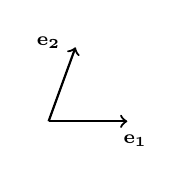
\begin{tikzpicture}
            \node at (1.1,-0.25) {\scriptsize $\vec{e_1}$};
            \draw[thick,->] (0,0) -- (0.342,0.940);
            \node at (0,1) {\scriptsize $\vec{e_2}$};
            \draw[thick,->] (0,0) -- (1,0);
        \end{tikzpicture}
    \caption{Any old basis $\vec{e}_n$} \label{fig:vectors-non-orth-1}
    \end{subfigure}
    \begin{subfigure}{0.5\textwidth}
        \centering
        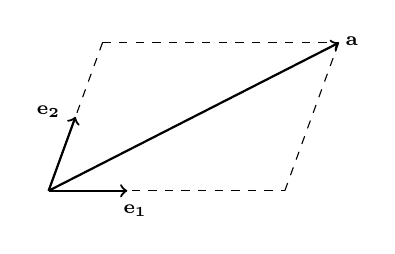
\begin{tikzpicture}
            \draw[dashed] (0,0) -- (3,0);
            \draw[dashed] (3,0) -- (3.684,1.879);
            \draw[dashed] (0,0) -- (0.684,1.879);
            \draw[dashed] (0.684,1.879) -- (3.684,1.879);
            \node at (1.1,-0.25) {\scriptsize $\vec{e_1}$};
            \draw[thick,->] (0,0) -- (0.342,0.940);
            \node at (0,1) {\scriptsize $\vec{e_2}$};
            \draw[thick,->] (0,0) -- (1,0);                    
            \draw[thick,->] (0,0) -- (3.684,1.879);
            \node at (3.85,1.9) {\scriptsize $\vec{a}$};
        \end{tikzpicture}
        \caption{$\vec{a} = \vec{e}_1 a^1 + \vec{e}_2 a^2$} \label{fig:vectors-non-orth-2}
    \end{subfigure}
\end{figure}

The problem comes when we try to recover the coordinates by projecting $\vec{a}$ onto the two basis vectors (Figure \ref{fig:vectors-non-orth-3}).

\begin{figure}[h]
    \caption{Projecting a vector onto a carelessly chosen basis}
    \begin{subfigure}{0.5\textwidth}
        \centering
        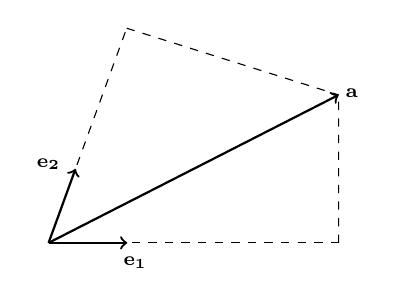
\begin{tikzpicture}
            \draw[dashed] (0,0) -- (3.684,0);
            \draw[dashed] (3.683,0) -- (3.684,1.879);
            \draw[dashed] (0,0) -- (0.992,2.726);
            \draw[dashed] (0.992,2.726) -- (3.684,1.879);
            \node at (1.1,-0.25) {\scriptsize $\vec{e_1}$};
            \draw[thick,->] (0,0) -- (0.342,0.940);
            \node at (0,1) {\scriptsize $\vec{e_2}$};
            \draw[thick,->] (0,0) -- (1,0);                    
            \draw[thick,->] (0,0) -- (3.684,1.879);
            \node at (3.85,1.9) {\scriptsize $\vec{a}$};
        \end{tikzpicture}
    \caption{Projecting $\vec{a}$ back onto the basis} \label{fig:vectors-non-orth-3}
    \end{subfigure}
    \begin{subfigure}{0.5\textwidth}
        \centering
        \begin{tikzpicture}
            \draw[dashed] (0,0) -- (3.684,-1.339);
            \draw[dashed] (3.683,-1.339) -- (3.684,1.879);
            \draw[dashed] (0,0) -- (0,3.218);
            \draw[dashed] (0,3.218) -- (3.684,1.879);
            \node at (1.2,-0.20) {\scriptsize $\vec{e^1}$};
            \draw[thick,->] (0,0) -- (0,1);
            \node at (-0.2,1.2) {\scriptsize $\vec{e^2}$};
            \draw[thick,->] (0,0) -- (0.992,-0.342);                    
            \draw[thick,->] (0,0) -- (3.684,1.879);
            \node at (3.85,1.9) {\scriptsize $\vec{a}$};
        \end{tikzpicture}
        \caption{$\vec{a} = a_1 \vec{e^1} + a_2 \vec{e^2}$} \label{fig:vectors-non-orth-4}
    \end{subfigure}
\end{figure}

We can visualise this projection process by drawing lines from the tip of $\vec{a}$ so they meet at right angles with the lines extended from the basis vectors. But these imply different coordinates for $\vec{a}$ from the ones that we used to build it using the basis $\vec{e}_n$.

This raises the question: in what basis are these the coordinates for $\vec{a}$? There is such a basis (Figure \ref{fig:vectors-non-orth-4}), $\vec{e^n}$, and we label the coordinates with subscripts, $a_n$, so the reconstructed $\vec{a}$ is given by:

$$
\vec{a} = a_1 \vec{e^1} + a_2 \vec{e^2}
$$

This basis $\vec{e}_j$ is related to the original basis $\vec{e}^i$ by \eqref{eqn:dual-bases-delta}. Looking at it geometrically (that is, cheating), when choosing the dual basis vector for a given index, we must choose a vector that is visibly orthogonal to all the other basis vectors, and this means we will have a severely limited choice, because there can be only one alignment that meets this requirement. Furthermore the magnitude of the vector $\vec{e}^i$ is fully determined by the requirement that $\langle \vec{e}_i, \vec{e}^i \rangle = 1$, as the ratio between the coordinates is already fixed by the choice of alignment.

In this visualisation process we have shown the relationship between $V$ and $V*$ by overlaying them on the same diagram, but they are in fact separate vector spaces: elements of $V$ are not elements of $V*$, and vice versa. But the way we have calibrated these two sets of bases to be mutually consistent is exactly the same as the relationship between the bases of $V$ and $V*$.

If the original basis vectors had been orthogonal, the dot product would have produced exactly the same coordinates we'd used to build the vector in the first place, i.e. figures \ref{fig:vectors-non-orth-2}, \ref{fig:vectors-non-orth-3} and \ref{fig:vectors-non-orth-4} would all be identical: a rectangle with the vector as its diagonal. But of course, we haven't yet said precisely what orthogonality means.

\subsection{The same ideas in coordinates}

We can make this concrete by playing with $\mathbb{R}^2$ as our vector space $V$, in which case the dual space of covectors $V^*$ contains mappings $\mathbb{R}^2 \mapsto \mathbb{R}$.

\begin{figure}[h]
    \caption{Basis vectors in $\mathbb{R}^2$}
    \begin{subfigure}{0.5\textwidth}
        \centering
        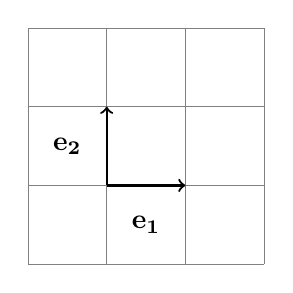
\begin{tikzpicture}
            \draw[step=1cm,gray,very thin] (1,1) grid (4,4); 
            \draw[thick,->] (2,2) -- (3,2);
            \node at (2.5,1.5) {$\vec{e_1}$};
            \draw[thick,->] (2,2) -- (2,3);
            \node at (1.5,2.5) {$\vec{e_2}$};        
        \end{tikzpicture}
        \caption{Orthonormality} \label{fig:vectors-orthonormality}
    \end{subfigure}
    \begin{subfigure}{0.5\textwidth}
        \centering
        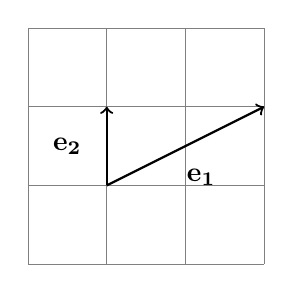
\begin{tikzpicture}
            \draw[step=1cm,gray,very thin] (1,1) grid (4,4); 
            \draw[thick,->] (2,2) -- (4,3);
            \node at (3.2,2.1) {$\vec{e_1}$};
            \draw[thick,->] (2,2) -- (2,3);
            \node at (1.5,2.5) {$\vec{e_2}$};
        \end{tikzpicture}
        \caption{Awkwardness} \label{fig:vectors-awkwardness}
    \end{subfigure}
\end{figure}

With our schoolhouse foreknowledge it would be easy to choose an orthonormal basis in $\mathbb{R}^2$ (Figure \ref{fig:vectors-orthonormality}):

$$
\vec{e}_1 = \begin{bmatrix}1 \\ 0\end{bmatrix}\,,\,
\vec{e}_2 = \begin{bmatrix}0 \\ 1\end{bmatrix}
$$

But we still haven't defined what orthonormal means, so we'll just choose something awkward (Figure \ref{fig:vectors-awkwardness}):

$$
\vec{e}_1 = \begin{bmatrix}2 \\ 1\end{bmatrix}\,,\,
\vec{e}_2 = \begin{bmatrix}0 \\ 1\end{bmatrix}
$$

By the way, it is customary to put the basis vectors in a row matrix, $\begin{bmatrix}\vec{e}_1 & \vec{e}_2\end{bmatrix}$, so they can be matrix-multiplied by a column representation of a vector in $V$, but that's not what we're doing here. We are giving the definition of each basis vector as a matrix, and the basis vectors are ordinary vectors belonging to $V$, so they must be column matrices.

What is the corresponding $V^*$ basis, $\vec{e}^i$? It has to obey:

$$
\langle \vec{e}_j,\vec{e}^i \rangle = \delta_{ij}
$$

Some straightforward equation building and substitution yields:

$$
\vec{e}^1 = \begin{bmatrix}0.5 & 0\end{bmatrix}\,,\,
\vec{e}^2 = \begin{bmatrix}-0.5 & 1\end{bmatrix}
$$

And these being covectors from $V^*$, they must be row matrices, as shown. Using our $V$ basis we can construct a vector $\vec{v}$ from the coordinates $(2, 3)$:

$$
\vec{v} = 2\vec{e}_1 + 3\vec{e}_2
        = \begin{bmatrix}4 \\ 2\end{bmatrix} + \begin{bmatrix}0 \\ 3\end{bmatrix} 
        = \begin{bmatrix}4 \\ 5\end{bmatrix}
$$

What happens if we evaluate the $V^*$ basis covectors against $\vec{v}$?

$$
\begin{bmatrix}0.5 & 0\end{bmatrix} \begin{bmatrix}4 \\ 5\end{bmatrix} = 2 
\,,\,
\begin{bmatrix}-0.5 & 1\end{bmatrix} \begin{bmatrix}4 \\ 5\end{bmatrix} = 3
$$

We get back the correct coordinates. If we'd just transposed the $V$ basis vectors into rows and left-multiplied them, we would have obtained wrong answers: this is precisely the same problem we saw with projecting onto the non-orthogonal basis.

But the utility of these basis covectors is limited to their ability to extract a scalar coordinate from a vector. For example, there is nothing here that generally relates any vector (other than the basis vectors) with a specific covector partner, or anything that relates one vector with another.

\section{Tensors}

Let's upgrade our black box machine so it has two input slots, accepting vectors $\vec{a}$ and $\vec{b}$ from the same vector space $V$, but still one output hole that gives us back a scalar $x$ (Figure \ref{fig:2-slot-box}).

\begin{figure}[h]
    \centering
    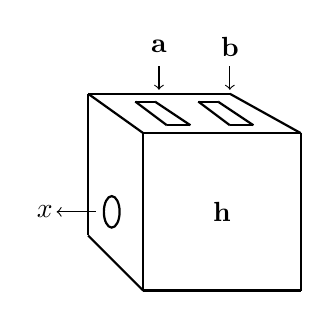
\begin{tikzpicture}
        \draw[thick] (0,0) -- (2,0);
        \draw[thick] (2,0) -- (2,2);
        \draw[thick] (2,2) -- (0,2);
        \draw[thick] (0,2) -- (0,0);
        \draw[thick] (0,2) -- (-0.7,2.5);
        \draw[thick] (-0.7,2.5) -- (-0.7,0.7);
        \draw[thick] (-0.7,0.7) -- (0,0);
        \draw[thick] (-0.7,2.5) -- (1.1,2.5);
        \draw[thick] (1.1,2.5) -- (2,2);

        \draw[thick] (1.4,2.1) -- (0.95,2.4);
        \draw[thick] (0.95,2.4) -- (0.7,2.4);
        \draw[thick] (0.7,2.4) -- (1.1,2.1);
        \draw[thick] (1.1,2.1) -- (1.4,2.1);

        \draw[thick] (0.6,2.1) -- (0.15,2.4);
        \draw[thick] (0.15,2.4) -- (-0.1,2.4);
        \draw[thick] (-0.1,2.4) -- (0.3,2.1);
        \draw[thick] (0.3,2.1) -- (0.6,2.1);
        
        \node at (0.2,3.1) { $\vec{a}$};
        \draw[->] (0.2,2.85) -- (0.2,2.55);

        \node at (1.1,3.1) { $\vec{b}$};
        \draw[->] (1.1,2.85) -- (1.1,2.55);

        \node at (-1.25,1) { $x$};
        \draw[thick] (-0.4,1) ellipse (0.1 and 0.2);
        \draw[->] (-0.6,1) -- (-1.1,1);

        \node at (1,1) { $\vec{h}$};

    \end{tikzpicture}
    \caption{Box $\vec{h}$ with two slots accepting vectors} \label{fig:2-slot-box}
\end{figure}

This is a mapping from pairs of vectors to scalars: $V \times V \mapsto \mathbb{R}$.

Suppose \textit{only to begin with} that the machine had an especially simple inner mechanism: inside the box $\vec{h}$, there are two single-slot boxes (covectors) $\vec{f}$ and $\vec{g}$. The machinery inserts input $\vec{a}$ into box $\vec{f}$, and input $\vec{b}$ into box $\vec{g}$, to obtain two scalars, which it simply multiplies together to produce its own resultant scalar that falls out of the hole of $\vec{h}$. In other words, it's really just two covectors glued together by scalar multiplication, and they act independently on the inputs:

$$
h(\vec{a}, \vec{b}) = \langle \vec{f},\vec{a} \rangle \langle \vec{g},\vec{b} \rangle
$$

In fact this design only accounts for a subset of the machines, but it will serve as an intuitive building block for us to construct all the machines we're interested in. We can write it as $\vec{f} \otimes \vec{g}$, which is called the \textit{tensor product} of the two covectors.

So sticking with this simplified design to begin with, consider the space of all such machines containing two covectors. We can define addition and scaling on these pairs in a way that satisfies the requirements of a vector space. Addition is easy. Much as we defined addition for covectors by simply adding their results when given the same input vector, we'll add these two-slot machines by adding their results when they act on the same pair of vectors:

\begin{equation}
\begin{split}
    (\vec{f} \otimes \vec{g} + \vec{p} \otimes \vec{q})(\vec{a}, \vec{b}) 
    &= 
    \vec{f} \otimes \vec{g} (\vec{a}, \vec{b}) + \vec{p} \otimes \vec{q}(\vec{a}, \vec{b}) \\
    &= \langle \vec{f}, \vec{a} \rangle
        \langle \vec{g}, \vec{b} \rangle
    + \langle \vec{p}, \vec{a} \rangle
        \langle \vec{q}, \vec{b} \rangle    
\end{split}        
\end{equation}

Scaling by some $x$ is even easier:

$$
\left[x(\vec{f} \otimes \vec{g})\right](\vec{a}, \vec{b}) 
= x(\vec{f} \otimes \vec{g})(\vec{a}, \vec{b}) 
= x \langle \vec{f}, \vec{a} \rangle
    \langle \vec{g}, \vec{b} \rangle
$$
 
Thus we have defined a vector space, and so these two-slot machines are also vectors. We can form a basis for that space by taking all possible pairs of basis covectors, $\vec{e}^i \times \vec{e}^j$. If the (co)vector space is $N$-dimensional, the pair-space will be $N^2$-dimensional, because it requires $N^2$ basis machines to span the space. Any two-slot machine can therefore be written as a linear combination (a weighted sum) of all the basis machines:

$$
\sum_{ij} M_{ij} (\vec{e}^i \otimes \vec{e}^j)
$$

And therefore to describe any two-slot machine in terms of the basis we will need $N^2$ numbers, which we can write as $M_{ij}$. By the way, there's no pressing need to think of it as a matrix, although we sometimes do. The $M$ stands for "machine" in this case. It's just a list of $N^2$ numbers, labelled with two indices that each can take on $N$ integer values, supplying the weighting for each basis machine.

Inserting two vectors $\vec{a}$ and $\vec{b}$ into the slots just means:

$$
\sum_{ij} M_{ij} \langle \vec{e}^i,\vec{a} \rangle \langle \vec{e}^j,\vec{b} \rangle
$$

Recall that an expression like $\langle \vec{e}^i,\vec{a} \rangle$ is the scalar resulting from $\vec{e}^i$ acting on $\vec{a}$. But as the input vector $\vec{a}$ can be described using the same (dual) basis, $a^k \vec{e}_k$: 

$$
\sum_{ijk} M_{ij} \langle \vec{e}^i, a^k \vec{e}_k \rangle \langle \vec{e}^j,\vec{b} \rangle
$$

and the same for $\vec{b}$:

$$
\sum_{ijkl} M_{ij} \langle \vec{e}^i, a^k \vec{e}_k \rangle \langle \vec{e}^j,b^l \vec{e}_l \rangle
$$

Both these substitutions required us to introduce a new summation index, because we are essentially "multiplying out" between the existing expression's summation terms and those of the vector we are substituting. So if the vector space is $2$-dimensional, the above is summing $2 \times 2 \times 2 \times 2 = 16$ terms. By linearity:

$$
\sum_{ijkl} M_{ij} a^k \langle \vec{e}^i, \vec{e}_k \rangle b^l \langle \vec{e}^j, \vec{e}_l \rangle
$$

We know the basis covectors acting on the basis vectors have very simple results by definition: $\langle \vec{e}^i, \vec{e}_k \rangle$ evaluates to $1$ if $i = k$, but is $0$ otherwise. Likewise $\langle \vec{e}^j, \vec{e}_l \rangle$ is $1$ if $j = l$ but $0$ otherwise. Therefore the $12$ summation terms where either $i \ne k$ or $j \ne l$ must vanish, leaving only $4$ terms where they are equal and the covector-vector interactions are simply replaced with $1$. Therefore we can replace $k$ with $i$ and $l$ with $j$ throughout:

\begin{equation}
    \sum_{ij} M_{ij} a^i b^j
        \label{eqn:two-slot-computation}
\end{equation}

So to compute the scalar result we only need the coordinates of the two input vectors and a list of numeric parameters that fully defines how the machine operates, creating summation terms that contribute various weightings of every possible combination of coordinates from the two vectors.

This kind of machine is called a \textit{tensor}.

It will often be the case that $M_{ij} = M_{ji}$, which is quite a lot of redundancy. But this is necessary to ensure that the machine is symmetrical: switching the inputs around does not affect the result. Of course, a machine doesn't have to be defined that way.

\subsection{Simple tensors}

We mentioned at the start that the simplified design (the ordinary product of two scalars obtained by two covectors operating separately on one vector input each) is not powerful enough to describe all these machines, even though we used it to define our basis machines. The simplistic machine is defined by a matrix that can be written as:

$$
M_{ij} = f_i g_j
$$

In other words, it can be decomposed into two separate columns of numbers. Such a machine is known as a \textit{decomposable}, \textit{elementary} or just \textit{simple} tensor.

One hint as to why it is so limited is that as $f_i$ and $g_j$ provide $N$ values each for an $N$-dimensional space, that is only $2N$ adjustable parameters, even though $M$ appears to have $N^2$ independent values. So we aren't allowing the full flexibility of which $M$ is capable.

Of course, if $N=2$ then $N^2 = 2N = 4$, but even then, there is a restrictive pattern that applies regardless of the dimensions. Viewing $M_{ij}$ as a matrix, every row (labelled by $i$) would be a scaled version of the numbers in $g_j$, and every column (labelled by $j$) would likewise be a scaled version of the numbers in $f_i$. That is, the rows are all linearly dependent on one another, and so are the columns. This would not be the case if the elements of $M$ were truly independent.

There's a subtlety here though: vector addition and scaling operators are meant to be closed. We've proposed a way of defining simple machines, which is a restricted set of objects, and then we've said that scaling and adding simple machines allows us to discover objects that are not in that simple set, which sounds like we're breaking the rules, reaching outside the initial set.

The resolution to this conundrum is that we are dealing with a general set of machines that can be described by the somewhat misleading notation $V^* \otimes V^*$, which we define as not only the simple machines made of any two covectors $f \otimes g$, but also those machines that are \textit{weighted sums} of one or more simple machines. This broader set includes machines that cannot be decomposed into two covectors. We can however choose a basis from the subset that \textit{can} be decomposed, and we do that because it is that subset for which we are able to directly explain how they operate. And from that basis we can build any machine of the form $V^* \otimes V^*$. Covectors (one-slot machines) are the most basic building block, from which we can make simple (two-slot) machines, from which in turn we can make any machines by linear combination of simple machines.

\subsection{Any number of slots}

Another point to note about these two-slot machines is that although here we focused on $V^* \otimes V^*$, we could instead of chosen $V \otimes V$, in which case the simple machine would have consisted of two vectors, and would have acted on two input covectors (recall how the notation $\langle \vec{f}, \vec{a} \rangle = \langle \vec{a}, \vec{f} \rangle$ emphasises symmetry, so we can think of a covector acting on a vector or a vector acting on a covector with no real difference in the result). We can define machines of the form: 

$$
V \otimes V^* \otimes V \otimes \ldots
$$ 

having any number of slots accepting any mixture of vectors and covectors in some specific order. A machine with five slots will be represented by a list of numbers labelled with five indices. The slots that accept vectors (being defined by covectors) will have down indices, and the slots that accept covectors (being defined by vectors) will have up indices. For example, we can say our machine is from the space:

$$
V \otimes V^* \otimes V \otimes V \otimes V^*
$$ 

or we can say it is represented by the numerical parameters:

$$
M\indices{^i_j^k^l_m}
$$

These convey the same information. Sometimes the indexed parameter notation is used as a compact way to describe the structure of the machine, the only downside being that we have to unnecessarily choose symbols for the indices.\footnote{Some authors call this \textit{slot-naming index notation}.}

\subsection{What is a tensor?}

These machines are tensors, though as we've seen, the space of machines of a given type is also a vector space, so tensors are vectors.

We have proposed creating a five-slot machine $M\indices{^i_j^k^l_m}$, and so it seems entirely proper to treat a 1-slot machine $M_i$ or $M^i$ as part of the same family of objects. We've been calling them covectors and vectors, which is accurate (we had to invent them first in order to build toward tensors), but they are also themselves tensors in this general sense.

Perhaps more surprising, but no less consistent, is the idea that a machine with no slots also belongs to the same family. It's just a scalar value.

Sometimes the type of a tensor is written $(u, d)$ where $u$ tells you how many up indices and $d$ tells you how many down indices it has. So a scalar is a $(0, 0)$-tensor, a vector is a $(1, 0)$-tensor, a covector is a $(0, 1)$-tensor, and we will soon encounter practical uses for $(1, 1)$, $(0, 2)$ and $(2, 0)$-tensors, all of which are also elements of vector spaces.

In summary, everything is seemingly an example of everything else, and yet all are different things.

\subsection{Contraction} \label{tensor-contraction}

When we insert a vector or covector into a suitable slot of a machine, we are effectively merging two tensors, by "wiring up" them up so that they share an index variable, which makes that variable disappear due to summation over it.

Starting with a five-slot machine $M\indices{^i_j^k^l_m}$ (which incidentally is a $(3,2)$-tensor), we will insert a covector $a_k$ into the middle slot, resulting in a machine $N$ with four slots (a $(2,2)$-tensor):

$$
N\indices{^i_j^l_m} = \sum_{k} M\indices{^i_j^k^l_m} a_k
$$

The index $k$ effectively disappears. This process is more formally regarded as a two stage process. First, we form the tensor product, which is an object with a separately named index for every index of the two source tensors:

$$
P\indices{^i_j^k^l_m_n} = M\indices{^i_j^k^l_m} a_n
$$

This step doesn't involve any summation. If the vector space is 4-dimensional, $P$ is a list of $4^6 = 4096$ numbers, each being the product of a distinct pair from the $4^5 = 1024$ numbers in $M$ and the $4$ numbers in $a$.

Then we link two of the slots by giving them the same index name and summing over that index (in this case by renaming $n$ to $k$):

$$
N\indices{^i_j^l_m} = \sum_{k} P\indices{^i_j^k^l_m_k}
$$

It's that second step, renaming $n$ to $k$ and summing over $k$, that is the actual contraction. We could then perform two contractions at once on $N$:

$$
x = \sum_{il} N\indices{^i_i^l_l}
$$

Each contraction ties two indices together and eliminates them, so this last double-contraction has eliminated four indices at once, leaving us with a scalar.

\section{Einstein notation}

We have been following a rule where basis vectors are given subscript indices, while vector components are given superscript indices. Then we do the opposite with basis covectors and components. This means that whenever one basis object acts on another:

$$
\langle e^i, e_j \rangle
$$

they always have opposing index positions. This is mirrored exactly by the way components are allowed to be multiplied. We've found that the dot product is only valid between the coordinates of a vector and a covector, so a product like this inside a summation, where we have repeated the same index variable:

$$
a^i b_i
$$

is valid, but neither of these is allowed because they imply a dot product between two vectors or two covectors:

$$
a^i b^i \, , \, a_i b_i
$$

Here's a real example that we'll encounter later:

$$
\sum_{\mu\nu\beta\lambda} g_{\mu\nu} Z\indices{^\mu_\beta} \underline{a}^{\beta} Z\indices{^\nu_\lambda} \underline{b}^{\lambda}
$$

Every single one of the four indices appears in two places, once up and once down. This immediately tells us that the result is a scalar. A simpler example shows how index variables are not necessarily introduced by summation:

$$
b^\mu = \sum_{\nu} O\indices{^\mu_\nu} a^\nu
$$

The $\nu$ index is repeated up/down in the way that is characteristic of all summation variables, but $\mu$ is introduced on the left to indicate that the expression computes the value of one component of several that represent a vector (we know it's a vector because the index is up).

From these patterns we can deduce something surprising: it is completely unnecessary to write the summation symbol and state what the summation index variables are! If an expression consisting indexed quantities multiplied together contains exactly two references to the same index, once up and once down, then that index is a summation index.

$$
g_{\mu\nu} Z\indices{^\mu_\beta} \underline{a}^{\beta} Z\indices{^\nu_\lambda} \underline{b}^{\lambda}
=
\sum_{\mu\nu\beta\lambda} g_{\mu\nu} Z\indices{^\mu_\beta} \underline{a}^{\beta} Z\indices{^\nu_\lambda} \underline{b}^{\lambda}
$$

$$
b^\mu = O\indices{^\mu_\nu} a^\nu = \sum_{\nu} O\indices{^\mu_\nu} a^\nu
$$

This shorthand applies just as well to basis vectors:

$$
\vec{a} = a^i \vec{e}_i = \sum_{i} a^i \vec{e}_i
$$

The recent example of a tensor product cannot be mistaken for an implied summation because there are no repeated indices:

$$
P\indices{^i_j^k^l_m_n} = M\indices{^i_j^k^l_m} a_n
$$
 
Whereas the contraction example unmistakably sums over $k$ alone:

$$
N\indices{^i_j^l_m} = P\indices{^i_j^k^l_m_k}
$$

Einstein came up with this abbreviation while developing General Relativity.

\section{The Inner Product}

The most important necessity for a specific machine of the form $V^* \otimes V^*$ is to at last come up with a way to define orthogonality, and the norm (length) of a vector, and thus orthonormality, but also a specific two-way pairing between every vector and a covector partner.

Nominating one such machine for a given vector space, we can call it the \textit{inner product}, and we say that the combination of the vector space and its inner product is an \textit{inner product space}.

As we've incessantly complained, we have so far had no way to judge whether two vectors are orthogonal to one another, even though we know that for arrows or column vectors there are some intuitive ways to choose orthogonal vectors. In our abstract development of the subject there was no such thing as orthogonal or orthonormal.

The choice of an inner product determines which vectors are mutually orthogonal, and also which are normalised (of unit norm). Importantly, it will also pair every vector with a single dual covector (and vice versa).

The notation $(\vec{a},\vec{b})$ is sometimes used for the inner product, similar to but deliberately distinct from the $\langle \vec{f},\vec{a}\rangle$ notation for the action of a covector on a vector.\footnote{Sadly the meanings of these notations are sometimes switched, and they aren't the only notations used.}

As it's a two-slot machine, its coordinate representation can be thought of as a matrix or a list of numbers addressed by two indices, and it is called the \textit{metric}. In General Relativity the metric is usually written as $g$, and its indices are often $\mu$ and $\nu$, so applying it to vectors $\vec{a}$ and $\vec{b}$ will look like this:

$$
(\vec{a},\vec{b}) = \sum_{\mu\nu} g_{\mu\nu} a^\mu b^\nu
$$

Or expressed in matrix multiplication, we put one of the vectors on the left of the matrix, transposed into a row, and one on the right as a column.

$$
(\vec{a}, \vec{b}) =
\begin{bmatrix}
a^1 & a^2 & a^3
\end{bmatrix}
\begin{bmatrix}
g_{11} & g_{12} & g_{13} \\
g_{21} & g_{22} & g_{23} \\
g_{31} & g_{32} & g_{33}
\end{bmatrix}
\begin{bmatrix}
b^1 \\ b^2 \\ b^3
\end{bmatrix}
$$

The central square matrix is always symmetric, $g_{\mu\nu} = g_{\nu\mu}$, so the vector inputs can be switched without affecting the result. The square matrix can multiply with the right column first, or with the left row: the order of operations doesn't matter.

As we will eventually see, this transposition business will wind up being somewhat messier than simply writing down the summations, in which the symmetry is a lot more obvious. This is one reason why it may not be worth thinking of $g$ (or any other two-slot machine) as a matrix.\footnote{Another reason: what if the machine has three or more slots?}

Compare it to the familiar dot product, which would be:

$$
\vec{a} \cdot \vec{b} = \sum_{\mu} a^\mu b^\mu
$$

It's the same row/square/column matrix multiplication except the central square matrix is missing, or equivalently it's the identity matrix:

$$
(\vec{a}, \vec{b}) =
\begin{bmatrix}
a^1 & a^2 & a^3
\end{bmatrix}
\begin{bmatrix}
1 & 0 & 0 \\
0 & 1 & 0 \\
0 & 0 & 1
\end{bmatrix}
\begin{bmatrix}
b^1 \\ b^2 \\ b^3
\end{bmatrix}
$$

So all the times when you obediently used the dot product to operate on two vectors, you were implicitly setting $g$ to be the Kronecker delta (§\ref{def:Kronecker}):

$$
g_{\mu\nu} = \delta_{\mu\nu}
$$

\textit{By definition} if the inner product is represented by $\delta_{\mu\nu}$ then the basis vectors are orthonormal. In other words, the inner product being represented by the identity matrix doesn't really tell us anything about the inner product. It tells us that we've chosen a set of basis vectors so that they are orthonormal according to this space's nominated inner product. It is always possible to do this, regardless of what the inner product happens to be.\footnote{Strictly speaking it is always possible for a finite-dimensional inner product space.}

This means that if we can use a single inner product consistently, we may as well define the basis to be orthonormal according that inner product, which means we will always be able to use the dot product between vectors, and the distinction between vectors and covectors becomes unimportant. We can even define all other multi-slot machines in terms of vectors acting on other vectors (via the inner product). That is, every machine would be of the form $V \otimes V \otimes V \otimes \ldots$, and would accept vectors as inputs.

This also means that the previous examples of what we called awkward basis vectors would in fact be orthonormal if we chose a particular inner product.

\subsection{No such thing as awkward}

Starting with the standard basis in column vectors, we could specify this as the inner product:

$$
g_{\mu\nu} = 
\begin{bmatrix}
\frac{1}{2} & -\frac{1}{2} \\
-\frac{1}{2} & 1
\end{bmatrix}
$$

We had to pick \textit{some} basis as a starting point or we would not have had a way to write down the inner product in numerical form. We used the standard basis, which is made of very simple one-hot vectors, but we now know that we must not call those vectors orthonormal.

Now we'll move the goalposts and choose a different set of vectors to be our basis, and they will be our usual awkward choice:

$$
\vec{e}_1 = \begin{bmatrix}2 \\ 1\end{bmatrix}\,,\,
\vec{e}_2 = \begin{bmatrix}0 \\ 1\end{bmatrix}
$$

Let's test our inner product on every possible pairing of these basis vectors:

$$
(\vec{e}_1, \vec{e}_1) =
\begin{bmatrix}
2 & 1
\end{bmatrix}
\begin{bmatrix}
\frac{1}{2} & -\frac{1}{2} \\
-\frac{1}{2} & 1
\end{bmatrix}
\begin{bmatrix}
2 \\ 1
\end{bmatrix}
= 1
$$    

$$
(\vec{e}_1, \vec{e}_2) =
\begin{bmatrix}
2 & 1
\end{bmatrix}
\begin{bmatrix}
\frac{1}{2} & -\frac{1}{2} \\
-\frac{1}{2} & 1
\end{bmatrix}
\begin{bmatrix}
0 \\ 1
\end{bmatrix}
= 0
$$    

$$
(\vec{e}_2, \vec{e}_1) =
\begin{bmatrix}
0 & 1
\end{bmatrix}
\begin{bmatrix}
\frac{1}{2} & -\frac{1}{2} \\
-\frac{1}{2} & 1
\end{bmatrix}
\begin{bmatrix}
2 \\ 1
\end{bmatrix}
= 0
$$    

$$
(\vec{e}_2, \vec{e}_2) =
\begin{bmatrix}
0 & 1
\end{bmatrix}
\begin{bmatrix}
\frac{1}{2} & -\frac{1}{2} \\
-\frac{1}{2} & 1
\end{bmatrix}
\begin{bmatrix}
0 \\ 1
\end{bmatrix}
= 1
$$    

The basis is orthonormal if $(\vec{e}_i, \vec{e}_j) = \delta_{ij}$. Undeniably, these basis vectors are orthonormal. The inner product says so, and who are we to doubt it? Furthermore, the inner product's matrix \textit{when expressed in this basis} is $\delta_{\mu\nu}$.

Every distinct basis provides a different way to describe any vector with coordinates, and likewise any covector. Regardless of the basis they are described in, the result of applying a specific covector to a specific vector will be the same scalar value. That is, the choice of basis is not a fact about the vector space, but merely a way to describe the vectors in it.

Choosing a different inner product (or equivalent, a metric) is not like that. In fact a given physical situation may impose a metric and we have to accept it; it's a fact of nature. So there are two possible reasons why the matrix $g_{\mu\nu}$ might change:

\begin{itemize}
    \item a change of basis, which will change the coordinates $a^{\mu}$ and $b^{\nu}$ of the two input vectors, as well as the matrix elements $g_{\mu\nu}$, so as to ensure the scalar result of the inner product $(\vec{a}, \vec{b})$ is unchanged, or
    \item a change of inner product itself, which will not affect the coordinates of anything else, and thus the scalar result of $(\vec{a}, \vec{b})$ may be very different.
\end{itemize}

\subsection{The metric and its inverse}

As always we must be careful not to confuse the coordinate or matrix representation of an object with the object itself. The matrix $g_{\mu\nu}$ is merely a representation in some basis of a machine with two slots awaiting vectors. 

We know that internal to that machine, it may be simple (consisting of two covectors, which are single-slot machines ready to operate on the two vectors inserted into the slots, and whose scalar results will be multiplied to get the result) or, more generally, it may be a linear combination of such simple two-slot machines.

Therefore if a single vector is inserted into the first slot, it will be fed into the first slot of one or more simple two-slot machines, which will all feed that same vector into their first covector. This will produce a set of scaling factors that apply to the second covector of each simple two-slot machine. This is in effect a set of single-slot machines being linearly combined into a single-slot machine (a weighted sum of covectors).

And we are left with a new single-slot machine awaiting another vector before it can produce a final scalar. In general a machine with $S$ slots can be nibbled away at sequentially, feeding in the $S$ inputs one at a time, each step reducing by one the capacity of the resultant machine to accept further inputs, until eventually all we are left with is a scalar result.

So as advertised, as well as providing a meaning for orthonormality, the metric also provides a complete pairing between every vector and a corresponding covector. Provide a single vector input to the metric and you will get back \textit{the} covector that is the dual partner to that vector, according to the metric.

It follows that if we find the inverse matrix to $g_{\mu\nu}$, that will act on a covector to reveal its dual vector. Or speaking abstractly, we can build something like the inner product but for getting a scalar from two covectors $(\vec{p}, \vec{q})$. Again the starting point is the simplest two-slot machine equivalent internally to two vectors $\vec{a}$ and $\vec{b}$. Each input covector is combined with one of the vectors and the two scalar results are multiplied together:

$$
(\vec{p}, \vec{q}) =
\langle \vec{p}, \vec{a} \rangle
\langle \vec{q}, \vec{b} \rangle
$$

And in general we would allow a linear combination of a basis formed from such simple machines, and of course this would have a matrix representation, because we will choose a vector basis $\vec{e}_{\mu}$, which will determine a covector basis $\vec{e}^{\mu}$:

$$
(\vec{f},\vec{g}) = \sum_{\mu\nu} g^{\mu\nu} p_{\mu} q_{\nu} 
$$

By our consistent use of subscript and superscript indices, we now have matrix representations for two forms of the inner product:

\begin{itemize}
    \item $g_{\mu\nu}$ operates on two vectors $a^{\mu}$ and $b^{\nu}$ to produce a scalar, or on one vector $a^{\mu}$ to produce its dual covector $p_{\mu}$.
    \item $g^{\mu\nu}$ operates on two covectors $p_{\mu}$ and $q_{\nu}$ to produce a scalar, or on one covector $p_{\mu}$ to produce its dual vector $a^{\mu}$. 
\end{itemize}

These operations can be performed in two stages. For example, $g_{\mu\nu}$ can first operate on $a^{\mu}$ to produce \textit{something} that is ready to operate on $b^{\nu}$ and finish the job by producing a scalar. That intermediate something, if it can act on a vector to get a scalar, must be a covector with coordinates $a_{\nu}$, one that is the dual of the vector it was produced from. If the basis happens to be orthonormal, the dual vector and covector will have the same coordinates, $a_{\mu} = a^{\mu}$ (because $g_{\mu\nu} = \delta_{\mu\nu}$).

So with reference to the indices being "up" or "down", $g^{\mu\nu}$ is sometimes called the raising operator, because it turns a covector's coordinates (subscript) into vector coordinates (superscript), while $g_{\mu\nu}$ is the lowering operator, working the other way. And described in this way, it is obvious that $g^{\mu\nu}$ undoes the work of $g_{\mu\nu}$, i.e. they are mutually inverse matrices. With our natural bias toward vectors, if $g_{\mu\nu}$ is the metric then $g^{\mu\nu}$ is the \textit{inverse metric}.

When dealing with objects expressed in coordinates we use the convention that vector coordinates are up and covector coordinates are down, and this lets us always take care to ensure that when we sum their products we always pair a vector (up) with a covector (down) using the same index variable. If necessary we can easily raise or lower using the appropriate version of the metric.

\section{Operators}

In this context, an operator $\hat{O}$ is a function that maps from a vector to a vector, $V \mapsto V$. As usual we are particularly interested in linear operators, for which:

$$
\hat{O} \vec{a}
=
\hat{O}\left(\sum_n a^n\vec{e}_n \right)
= 
\sum_n a^n\hat{O}\vec{e}_n
$$

Why? Because to completely characterise the behaviour of such an $\hat{O}$ we only need to know its effect on the $n$ basis vectors, which we can capture in a square matrix.

This is a new kind of geometric object. It has a physical meaning that is entirely independent of the choice of basis, even though the matrix elements will certainly be different depending on the basis. So just as we can speak of the same vector being represented by different columns of coordinates depending on the choice of basis, we can also speak of the same operator being represented by matrices of different elements depending on the choice of basis.

When we label a matrix with indices, $M_{ij}$, we have choice: should they be subscript or superscript? This was straightforward when we introduced the inner product, because we conceived of it as two covectors tied together by multiplication: $V^* \otimes V^*$, and so their coordinate representations must have subscripts, and hence the metric has subscript indices. Likewise the inverse metric is like two vectors, $V \otimes V$, and so has superscript indices.

In both those cases, we found that as well as acting as a mapping from two inputs to a scalar, the same object could map a single input to its dual partner.

Here we want a machine that maps a vector to a vector. As a hunch, consider the set of $V \otimes V^*$ machines. Such a machine will be a linear combination of simple machines made of a vector and a covector, $\vec{a} \otimes \vec{f}$:

\begin{equation}
\hat{O} = \sum_{\mu\nu} O\indices{^\mu_\nu} \left( \vec{e}_\mu \otimes \vec{e}^\nu \right)
\end{equation}

So the operator is represented (in the current basis) by a matrix with one super and one sub index, being the sum of a set of matrices whose elements are the product of a vector coordinate and a covector coordinate. To find the coordinates of the resultant vector $\vec{b}$ obtained from $\hat{O} \vec{a}$:

$$
b^\mu = \sum_{\nu} O\indices{^\mu_\nu} a^\nu
$$

There are some operators that have the same coordinates in all bases. The $0$-matrix, which maps all vectors to the $0$-vector, has all its elements $0$. The identity operator, which has no effect on its input, is $\delta_{\mu\nu}$ in all bases.

We can think of a vector as pointing in a direction in space, and this being an aspect of its geometrical nature. How can we similarly characterise operators?

\section{Eigenvectors and Eigenvalues}\label{sec:vectors-eigen}

An operator that performs only scaling is isotropic, treating all directions equivalently. We can (in somewhat woolly terms) think of it as sphere-shaped.

But some operators are biased with regard to direction. To characterise the behaviour of an operator we can consider those vectors which are scaled by it without their direction being altered (the scaling may be negative, leaving the vector pointing the opposite direction; as long as the resulting vector is co-linear with the input vector, that's insignificant enough.) Such vectors are called the \textit{eigenvectors} of the operator, and the scaling value associated with each eigenvector is called an \textit{eigenvalue}. Note that the zero vector is not considered a candidate for an eigenvector. It has no direction, making it impossible to say whether the operator has changed its direction. Also it goes from length zero to length zero under any operator, so any scalar could be the eigenvalue, meaning that the eigenvalue is undefined.

For operators that perform a general isotropic scaling, all input vectors are eigenvectors: all inputs get only scaled, and always by the same eigenvalue.

With vectors in the plane, when the operator is a pure rotation, e.g. by a right-angle anti-clockwise:

$$R_A = \begin{bmatrix}0 & -1 \\ 1 & 0\end{bmatrix}$$

or clockwise:

$$R_C = \begin{bmatrix}0 & 1 \\ -1 & 0\end{bmatrix}$$

every vector changes direction by the same angle, and that means there are no eigenvectors.

More interestingly, there are operators for which only some vectors are eigenvectors. In three dimensions the rotation has an axis, along which all vectors are eigenvectors, and any vectors not on that axis are not eigenvectors. Curiously, even though these eigenvectors don't exist in the planar case, we can find \textit{complex} eigenvalues for them by supposing that such eigenvectors exist, which is weird.

Consider a reflection (call it $M$ for mirror):

$$M = \begin{bmatrix}1 & 0 \\ 0 & -1\end{bmatrix}$$

If we take the first coordinate to be horizontal and the second vertical, this flips the input vector to point up rather than down, or vice versa. So it seems that all vectors have their direction changed and are not eigenvectors, but there exceptions: vectors that lie on the horizontal axis and have no vertical component will be unaffected, i.e. they will be eigenvectors with eigenvalue 1. Also vectors that lie on the vertical axis will have their direction changed, but to the exact opposite direction (their alignment does not change), which is the same as being scaled by -1, and so these too are eigenvectors, but with eigenvalue -1.

So within the space of input vectors, there is a subspace (the \textit{eigenspace}) of eigenvectors, and $M$ has an intrinsic orientation, as there is a particular line around which reflection occurs.

We can find the eigenvectors given a matrix representation $M$ of an operator acting on a vector represented by a column matrix $v$. If $v$ is an eigenvector, and $x$ is the corresponding eigenvalue, what we mean by that is:

$$Mv = xv$$

For the vector $v$, multiplying it by the matrix $M$ is the same as multiplying it by the ordinary number $x$. So with trivial algebra:

$$Mv - xv = 0$$

This is fine because $Mv$ and $xv$ are column matrices, and here $0$ is the column matrix filled with zeros.

Pulling out $v$ as a factor (not quite as trivial):

$$(M - xI)v = 0$$

We have to leave behind the identity matrix $I$ in place of $v$ because we need the matrix equivalent of the ordinary number $x$, so we can subtract it from $M$.

Having split it into two factors whose product is zero, we know that either one or both of the factors must be zero. We already realised we aren't interested in the case where $v$ is the zero vector because its eigenvalue will be undefined (it could be anything). So we refuse to accept $0$ as an eigenvector. Therefore $v$ is not the zero vector, and so the matrix $M - xI$ must be such that it is able to transform some non-zero vector $v$ into the zero vector. This means it has no inverse, as there is no way to recover the direction of the original vector if we've sent it to $0$ (the zero vector has no direction, or has all directions, so direction is a meaningless concept for it.)

Restricting ourselves to a two dimensional vector space, one way to picture the effect of a matrix is to think of it acting on a unit square (where the matrix is $2 \times 2$) and asking what the area of the resulting parallelogram will be. If it is not zero, every point in the original square has a unique point in the parallelogram and vice versa: the matrix is invertible. If the area is zero, the points of the original square have been crammed onto a line of $1$ dimension, so we have destroyed the information about where they came from in $2$ dimensions. All input vectors end up pointing in the same direction, and are only distinguished by length. No linear transform will be able to spread them back out into the correct different directions: the matrix is not invertible.

The area of that parallelogram (or in higher dimensions, the volume of an n-parallelepiped) is called the determinant of the matrix, $\det M$. If it's zero, the matrix is not invertible. And therefore, if:

$$\det{(M - xI)} = 0$$

then we definitely have some eigenvalues. The determinant can be expanded out into a polynomial expression in $x$ (there are various methods; a popular one is to get a computer to do it) and then solved by factoring to find all the $x$ values that make one of the factors $0$. We can then plug those $x$ values back into:

$$(M - xI)v = 0$$

one at a time, and solve to find the corresponding $v$. Thankfully all this can be mechanised.

\subsection{Symmetric Matrices}\label{ch:vectors-symmetric}

A matrix where $M^\intercal = M$, or $M_{ij} = M_{ji}$ is of particular interest. We've seen how it can be used to define an operation on two vectors that produces a scalar, such that the operation is symmetric (commutative).

Also it is possible to select from its eigenvectors a set that are orthogonal and completely span the vector space. That is, in an N dimensional space, they perform a scaling in all N available orthogonal directions, stretching or squishing. We need to be clear about what we mean by orthogonal, of course: this is a matrix in isolation from any defined geometric context, so we're talking about column vectors in the standard basis.

This is hugely important in Quantum Mechanics (§\ref{ch:qm}), albeit with some modifications for complex numbers.

\section{Change of Basis}\label{sec:vectors-change-basis}

We have now accumulated a menagerie of geometric objects that can be described numerically relative to a chosen basis. We now turn to the problem of what happens to the those numerical representations when we choose a different set of basis vectors.

Often in discussions of transformations a tick is added to existing symbols to indicate the transformed version of that symbol, e.g. $x$ becomes $x'$ (pronounced "x prime"). But this clashes horribly with superscripts. So here we will use underlining, e.g. the vector $\vec{a}$ may have a first representation in coordinates $a^i$ and also a transformed representation $\underline{a}^i$.

\subsection{Effect of change of basis on vectors}

A vector $\vec{v}$ in some basis can be expressed in coordinates as a column matrix $v$:

$$v = \begin{bmatrix}3 \\ 4\end{bmatrix}$$

Note that, unlike some prior examples, we are not saying the vector \textit{is} the column matrix. We are saying nothing at all about the nature of the vectors, except that they are elements of some vector space. We are describing in numbers a vector of unknown type taken from some vector space, which we can only do because we have chosen a basis, $e$:

$$e = \begin{bmatrix}\vec{e_1} & \vec{e_2}\end{bmatrix}$$

Matrix multiplication builds the vector:

$$\vec{v} = ev = 3\vec{e_1} + 4\vec{e_2}$$

We can create a matrix that will double the length of the basis vectors:

$$Z = \begin{bmatrix}2 & 0 \\ 0 & 2\end{bmatrix}$$

By the rules of matrix multiplication the bases must be on the left.

$$\underline{e} = eZ = \begin{bmatrix}2\vec{e_1} & 2\vec{e_2}\end{bmatrix}$$

What coordinates would $\vec{v}$ have in this new basis $\underline{e}$? Intuitively the coordinates need to be halved to refer to the same vector. So we need the inverse of $Z$, written as $Z^{-1}$, which shrinks the coordinates:

$$Z^{-1} = \begin{bmatrix}0.5 & 0 \\ 0 & 0.5\end{bmatrix}$$

And so our vector's coordinates become:

$$\underline{v} = Z^{-1}v = \begin{bmatrix}1.5 \\ 2\end{bmatrix}$$

This is the same vector as before, just in different coordinates:

$$\vec{v} = ev = \underline{e} \, \underline{v}$$

We say that vectors are \textit{contravariant} under a change of basis, because their coordinates are transformed by the inverse of the matrix used to transform the basis.

This shows how important it is to be clear about how we're defining the adjustment made to the basis. A transformation $Z$ applied to the basis vectors implies a transformation $Z^{-1}$ on the coordinates of vectors. So when we talk about similar effects on other objects, to avoid confusion we'll consistently start with $Z$, the transformation that updates the basis.

\subsection{Effect of change of basis on covectors} \label{sec:vector-grow-shrink}

A covector can be thought of as a yardstick or a measuring device. By evaluating it with some vector parameter, you are taking a measurement of that vector in the form of an ordinary number, something that is independent of any choice of basis and thus independent of the representation in coordinates.

The ordinary vector $\vec{x}$ is represented by a column matrix $x$ of coordinates in our initial basis. As we're updating the basis with $Z$, therefore we must left-multiply the coordinates of the vector by $Z^{-1}$ to get it in the new coordinate system:

$$
\underline{x} = Z^{-1} x
$$

But for the covector $\vec{f}$, which is a row matrix $f$, we right-multiply by the original $Z$ (not the inverse):

$$
\underline{f} = f Z
$$

This ensures that the two representations give us exactly the same numerical result when we evaluate the function on the vector, regardless of the basis:

$$
\langle \vec{f}, \vec{x} \rangle = \underline{f} \, \underline{x} = (f Z) (Z^{-1} x) = f (Z Z^{-1}) x = fx
$$

The scalar $\langle \vec{f}, \vec{x} \rangle$ is a basis-independent physical fact. To balance the effect of a coordinate transformation, whatever we do to the coordinates of our vectors, we must do the inverse to the coordinates of our covectors.

\subsection{The inner product under change of basis}

The inner product $g$ operates on two vectors. We've written it in matrix multiplication form by putting the transpose $a^\intercal$ of the first vector on the left, so it becomes a single row matrix, with the second vector on the right as a column matrix $b$:

$$
(\vec{a}, \vec{b}) = a^\intercal g\, b = \sum_{\mu\nu} a^{\mu} g_{\mu\nu} b^{\nu}
$$

If we transform the basis by $Z$, we know the coordinate columns $a$ and $b$ for the two vectors must transform by $Z^{-1}$ to become $\underline{a}$ and $\underline{b}$. To produce the same result, the metric square matrix $g$ must be replaced with a new matrix $\underline{g}$. 

$$
(\vec{a}, \vec{b}) = \underline{a}^\intercal \underline{g}\, \underline{b} = a^\intercal g\, b
$$

So in practical terms, we need a new two-slot machine $\underline{g}$ that hides the original $g$ machine in a compatibility layer, which "un-transforms" the two input vectors before passing them on to its concealed inner $g$.

To get $b$ back from $\underline{b}$ is easy, because we just left multiply by $Z$ to cancel out the $Z^{-1}$:

$$
b = Z(\underline{b}) = Z(Z^{-1}b) = (Z\,Z^{-1})b = b
$$

To get $a$ from $\underline{a}$ would be the same, except we want to get $a^\intercal$ from $\underline{a}^\intercal$, so instead we right-multiply by $Z^\intercal$, which looks awful but is really the same thing with everything transposed and with the order flipped:

$$
a^\intercal = (\underline{a}^\intercal)Z^\intercal = (a^\intercal (Z^{-1})^\intercal) Z^\intercal = a((Z^{-1})^\intercal) Z^\intercal) = a
$$

So un-transforming the left and right sides means we can use the unmodified $g$:

$$
(\vec{a}, \vec{b}) = (\underline{a}^\intercal Z^\intercal) g (Z \underline{b}) 
$$

But associativity means we can bracket the middle square matrix separately:

$$
(\vec{a}, \vec{b}) = \underline{a}^\intercal (Z^\intercal g Z) \underline{b} 
$$

And so:

$$
\underline{g} = Z^\intercal g Z
$$

By far the ugliest part of this was all the transposition on the left side. But we can avoid matrix notation entirely and use summation. We know that in the original basis:

$$
(\vec{a}, \vec{b}) = \sum_{\mu\nu} a^{\mu} g_{\mu\nu} b^{\nu}
$$

This clarifies that we're just adding a lot of products: $a^{\mu}$, $g_{\mu\nu}$ and $b^{\nu}$ are all just ordinary numbers that we're multiplying so although we've written them in the same order they appear in the matrix multiplication, that is entirely unnecessary here.

We've seen how a machine like $g$ can be defined as a linear combination of a set of basis machines that span the space of all possible machines, each basis machine being formed by choosing a distinct pairing of the basis covectors:

$$
\sum_{\mu\nu} g_{\mu\nu} (\vec{e}^i \otimes \vec{e}^j)
$$

And how that machine acts on two vectors like so:

$$
\sum_{\mu\nu} g_{\mu\nu} \langle \vec{e}^\mu,\vec{a} \rangle \langle \vec{e}^\nu,\vec{b} \rangle
$$

But this time we'll build the vectors $\vec{a}$ and $\vec{b}$ from their coordinates in the transformed basis, $\underline{a}^{i}$ and $\underline{b}^{i}$.

The basis is transformed by $Z$, and so the coordinates of the vectors will have been transformed by $Z^{-1}$, and thus to recover the coordinates in the original basis we'll have to use $Z$:

$$
\vec{a} = \sum_{\alpha\beta} Z\indices{^\alpha_\beta} \underline{a}^{\beta} \vec{e}_{\alpha}
\, , \,
\vec{b} = \sum_{\kappa\lambda} Z\indices{^\kappa_\lambda} \underline{b}^{\lambda} \vec{e}_{\kappa}
$$

By the usual substitution and linearity jiggling (yes, that's six indices, so $2^6 = 64$ summation terms if the space is $2$-dimensional):

$$
\sum_{\mu\nu\alpha\beta\kappa\lambda} g_{\mu\nu} Z\indices{^\alpha_\beta} \underline{a}^{\beta} Z\indices{^\kappa_\lambda} \underline{b}^{\lambda} \langle \vec{e}^\mu, \vec{e}_\alpha \rangle \langle \vec{e}^\nu, \vec{e}_\kappa \rangle
$$

But also as usual, most of the terms vanish because that's how basis covectors operate on basis vectors. We can replace $\alpha$ with $\mu$ and $\kappa$ with $\nu$, eliminating two indices:

$$
\sum_{\mu\nu\beta\lambda} g_{\mu\nu} Z\indices{^\mu_\beta} \underline{a}^{\beta} Z\indices{^\nu_\lambda} \underline{b}^{\lambda}
$$

Merely reordering and grouping so that the input vector coordinates are last:

$$
\sum_{\beta\lambda\mu\nu} \left[g_{\mu\nu} Z\indices{^\mu_\beta} Z\indices{^\nu_\lambda} \right] \underline{a}^{\beta} \underline{b}^{\lambda} 
$$

This is an example of a self-contained set of summed terms that can be extracted, by defining:

$$
\underline{g}_{\beta\lambda} = 
\sum_{\mu\nu} g_{\mu\nu} Z\indices{^\mu_\beta} Z\indices{^\nu_\lambda}
$$

Which is the rule for transforming $g$ to account for a basis transformation $Z$, giving us two ways to calculate the same inner product value:

$$
(\vec{a}, \vec{b})
= 
\sum_{\beta\lambda} \underline{g}_{\beta\lambda} \underline{a}^{\beta} \underline{b}^{\lambda}
= 
\sum_{\mu\nu} g_{\mu\nu} a^{\mu} b^{\nu}
$$

\subsection{Linear operators under change of basis}

We've just seen how to transform a matrix, $g$ into $g$, so now we know how to transform matrices, nothing to see here, move along, right?

A linear operator is a mapping $V \mapsto V$, whereas the inner product maps $V \mapsto V^*$. Among other observations, we saw that there is always a basis in which the inner product is represented by $g_{\mu\nu} = \delta_{\mu\nu}$, but if a linear operator is represented by $\delta_{\mu\nu}$ then it maps every vector to itself, and that means it must be represented by $\delta_{\mu\nu}$ \textit{regardless of the basis}. So they are not the same.




\section{Displacement in a scalar field}

\subsection{Temperature as a function of position}

We often have a scalar field (in the physics sense), that is, a scalar-valued function of position in space. An example is a survey of the temperature at points on a tabletop. This is highly unlikely to be a linear function of position. In one region of the table there is a hot cup of tea, and in another there is an ice bucket of champagne. The temperature is a complex, messy function of position.

We can then ask what by what amount does the temperature change if we move from our current position to another spot nearby. This temperature change is given by a scalar-valued function of the displacement vector (like a covector). Clearly this function has a different definition at each location. But to be accurate over any distance it would need to be arbitrarily complicated (unlike a covector)

\begin{figure}[h]
    \centering
    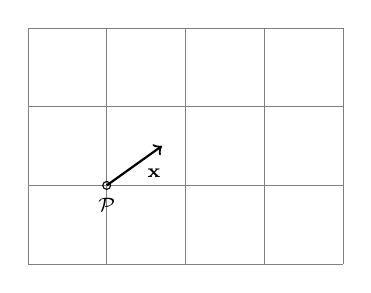
\begin{tikzpicture}
        \draw[step=1cm,gray,very thin] (0,0) grid (4,3);
        \node at (1,0.75) {\scriptsize $\mathcal{P}$};
        \draw (1,1) circle (0.05);
        \node at (1.6,1.15) {\scriptsize $\vec{x}$};
        \draw[thick,->] (1,1) -- (1.7,1.5);
    \end{tikzpicture}
    \caption{A small displacement from $\mathcal{P}$.} \label{fig:vector-displacement}
\end{figure}

The position of a point on the tabletop (Figure \ref{fig:vector-displacement}) is given by a position vector and the temperature by the function $T$. We start at the point $\mathcal{P}$, reached by the position vector $\vec{p}$, where the temperature is $T(\vec{p})$, and we want to know by how much the temperature will change if we move by a small displacement $\vec{x}$.

The answer is given by the function $dT(\vec{x})$, which will be a different function depending on where $\mathcal{P}$ is. We can sort of cheat and define it in terms of $T$ with perfect accuracy:

$$
dT(\vec{x}) = T(\vec{p} + \vec{x}) - T(\vec{p})
$$

But that would be overkill. All we really need is a linear approximation that is only precisely accurate at $\mathcal{P}$, where it has the value zero, but will change linearly with increasing distance (and may diverge from the truth). 

That is, for any scalar constant $k$:

$$
dT(k \vec{x}) = k \, dT(\vec{x})
$$

As $k$ shrinks, the error vanishes:

\begin{equation}
    dT(\vec{x}) = \lim_{k \to 0} \frac{T(\vec{p} + k\vec{x}) - T(\vec{p})}{k}
    \label{eqn:directional-derivative-limit}
\end{equation}

Having chosen a direction, the $dT$ function's value will be proportional to the distance moved, which is to say, the magnitude of the supplied displacement vector. The smaller the displacement, the smaller the value, but also the smaller the error. For large displacement it may be wildly wrong; it doesn't carry enough information about the shape of the temperature map contained in $T$ to reproduce it perfectly. It only knows something about how $T$ changes in the immediate vicinity of $\mathcal{P}$, but that's enough, because if $T$ is a complicated function then there will be a different $dT$ function associated with each point in space, and that variation will encode the underlying shape of $T$.

A function that maps vectors to scalars in this simple linear way is clearly a covector, $\vec{d}$. Given a covector basis $\vec{e}^n$, there will be a set of coordinates $d_n$:

\begin{equation}
    dT(\vec{x}) = \vec{d} = \sum_n \vec{e}^n d_n
    \label{eqn:covector-directional-derivative}
\end{equation}

For every covector there is a dual vector, from the vector space that we use to describe the displacement $x$, that we could use to convey the same information as $\vec{d}$. If we call that vector $\vec{s}$ (short for "slope", for reasons that may become clear), we know how to convert covector coordinates into vector coordinates with the inverse metric $g^{\mu\nu}$:

\begin{equation}
\begin{split}
\vec{s} 
&= \sum_{\mu} \left( \sum_{\nu} g^{\mu\nu} d_{\nu} \right) \vec{e}_{\mu} \\
&= \sum_{\mu} s_{\mu} \vec{e}_{\mu}
\label{eqn:vector-gradient}
\end{split}
\end{equation}

Of course just as the function $df$ (a.k.a. the covector $\vec{d}$) is different at each point in the physical space, so too is the corresponding vector $\vec{s}$. It's a vector field. The official name for $\vec{s}$ is the \textit{gradient}\footnote{We can't reasonably call it $\vec{g}$, as that is the metric (blame Gauss.)} of $T(x)$.

\subsection{Uniform gradient in orthonormal basis}

\begin{figure}[h]
    \caption{Simplified scalar field}
    \centering
    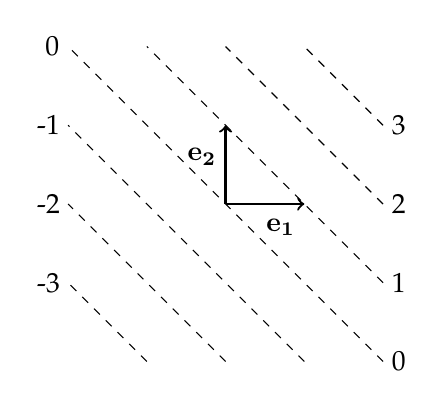
\begin{tikzpicture}
        \draw[dashed] (1,0) -- (0,1);
        \node at (-0.25,1) {-3};
        \draw[dashed] (2,0) -- (0,2);
        \node at (-0.25,2) {-2};
        \draw[dashed] (3,0) -- (0,3);
        \node at (-0.25,3) {-1};
        \draw[dashed] (4,0) -- (0,4);
        \node at (-0.2,4) {0};
        \node at (4.2,0) {0};
        \draw[dashed] (4,1) -- (1,4);
        \node at (4.2,1) {1};
        \draw[dashed] (4,2) -- (2,4);
        \node at (4.2,2) {2};
        \draw[dashed] (4,3) -- (3,4);
        \node at (4.2,3) {3};
        \draw[thick,->] (2,2) -- (3,2);
        \node at (2.7,1.7) {$\vec{e_1}$};
        \draw[thick,->] (2,2) -- (2,3);
        \node at (1.7,2.6) {$\vec{e_2}$};
    \end{tikzpicture}
    \label{fig:scalar-field-std-basis}
\end{figure}

To drastically simplify, we'll consider a scalar field that has the same gradient everywhere in space. This means that the temperature function of absolute position $T(\vec{p})$ depends in a simple way on the position. We can define it in familiar way by using the standard basis, that is, orthonormal basis vectors $\vec{e}_n$, which are shown in Figure \ref{fig:scalar-field-std-basis} overlaid on dashed lines of equal temperature.

The temperature as a function of the position coordinates $p^n$ is given by:

\begin{equation}
    T(\vec{p}) = p^1 + p^2
    \label{eqn:t-absolute}
\end{equation}

The temperature is simply the sum of the coordinates, and so at the origin the temperature is $0$, likewise at coordinates $(1, -1), (2, -2), (-1, 1), (-2, 2)$ and so on, which is to say that there is a diagonal line along which $T$ is $0$. Similarly there is a parallel line along which $T$ is $1$, another where it is $-1$ and so on. These lines are \textit{isolines} or \textit{contours}\footnote{Strangely they are sometimes called "contour lines" even if they are curved paths.}

The simplification arsing from a scalar field whose contours are evenly spaced parallel lines is that although $T$ changes with position, there is no variation in \textit{how it changes} with position. This means that the function $dT$ for the change made by a small displacement $\vec{x}$ is structurally identical to \eqref{eqn:t-absolute}:

\begin{equation}
    dT(\vec{x}) = x^1 + x^2
    \label{eqn:t-rel}
\end{equation}

(As always in this topic, $x^2$ means the second coordinate of a column vector, not the square of a variable $x$.) We can express this function in matrix multiplication:

\begin{equation}
    T(\vec{x}) = 
    \begin{bmatrix}1 & 1\end{bmatrix}
    \begin{bmatrix}x^1 \\ x^2\end{bmatrix}
    \label{eqn:t-rel-matrices}
\end{equation}

That is, it's the action of a covector with coordinates $(1, 1)$, which we called $\vec{d}$ in \eqref{eqn:covector-directional-derivative}:

$$
T(\vec{x}) = \langle \vec{d}, \vec{x} \rangle
$$

The dual of $\vec{d}$ is the vector we called $\vec{s}$ in \eqref{eqn:vector-gradient}, and because we're in the standard orthonormal basis the coordinates are the same, $d_n = s^n$. This is the gradient vector and can be legitimately drawn in physical space as a vector (Figure \ref{fig:gradient-vector}).

\begin{figure}[h]
    \caption{Gradient vector}
    \centering
    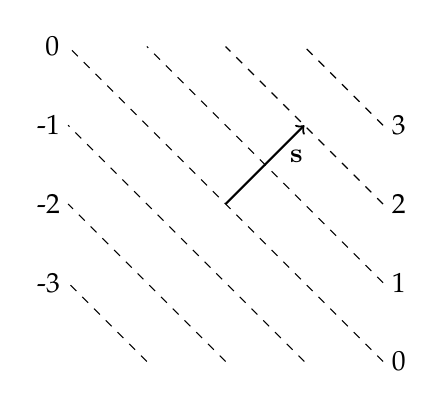
\begin{tikzpicture}
        \draw[dashed] (1,0) -- (0,1);
        \node at (-0.25,1) {-3};
        \draw[dashed] (2,0) -- (0,2);
        \node at (-0.25,2) {-2};
        \draw[dashed] (3,0) -- (0,3);
        \node at (-0.25,3) {-1};
        \draw[dashed] (4,0) -- (0,4);
        \node at (-0.2,4) {0};
        \node at (4.2,0) {0};
        \draw[dashed] (4,1) -- (1,4);
        \node at (4.2,1) {1};
        \draw[dashed] (4,2) -- (2,4);
        \node at (4.2,2) {2};
        \draw[dashed] (4,3) -- (3,4);
        \node at (4.2,3) {3};
        \draw[thick,->] (2,2) -- (3,3);
        \node at (2.9,2.6) {$\vec{s}$};
    \end{tikzpicture}
    \label{fig:gradient-vector}
\end{figure}

Note how it is perpendicular to the contours. It points in the direction of "steepest increase" of the field. Also its magnitude is significant: if you move $1$ unit of distance along the direction of $\vec{s}$, the field will increase by $\|\vec{s}\|$, which in this case is $\sqrt{2}$.

(The diagram is possibly confusing on this point, because it actually shows that a displacement by $\vec{s}$, i.e. moving along the direction of $s$ by distance $\|\vec{s}\|$, will increase $T$ by $2$, which is the same thing.)

\subsection{Uniform gradient in a non-orthonormal basis}

How can we be sure that this description wasn't affected by our use of the standard basis?

\begin{figure}[h]
    \caption{Simplified scalar field in another basis}
    \centering
    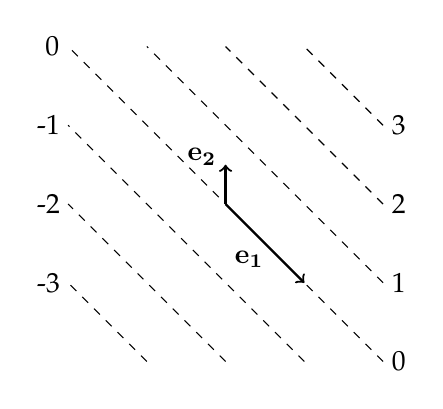
\begin{tikzpicture}
        \draw[dashed] (1,0) -- (0,1);
        \node at (-0.25,1) {-3};
        \draw[dashed] (2,0) -- (0,2);
        \node at (-0.25,2) {-2};
        \draw[dashed] (3,0) -- (0,3);
        \node at (-0.25,3) {-1};
        \draw[dashed] (4,0) -- (0,4);
        \node at (-0.2,4) {0};
        \node at (4.2,0) {0};
        \draw[dashed] (4,1) -- (1,4);
        \node at (4.2,1) {1};
        \draw[dashed] (4,2) -- (2,4);
        \node at (4.2,2) {2};
        \draw[dashed] (4,3) -- (3,4);
        \node at (4.2,3) {3};
        \draw[thick,->] (2,2) -- (3,1);
        \node at (2.3,1.3) {$\vec{e_1}$};
        \draw[thick,->] (2,2) -- (2,2.5);
        \node at (1.7,2.6) {$\vec{e_2}$};
    \end{tikzpicture}
    \label{fig:scalar-field-awkward-basis}
\end{figure}

Let's rewind back to the start and pick a different basis (Figure \ref{fig:scalar-field-awkward-basis}). We've changed $\vec{e}_1$ to point diagonally downwards and to the right, so in terms of the standard basis it would have coordinates $(1, -1)$. We've also made $\vec{e}_2$ half its previous length.

The significant thing about this (apart from the abandoning of both orthogonality and equal lengths) is that $\vec{e}_1$ is parallel to the contours. This means that a displacement that adjusts only the first coordinate will not affect the value of $T$, because it just moves along the current contour. But a displacement in the second coordinate will have half the effect it had before. So we expect:

\begin{equation}
    dT(\vec{x}) = \frac{1}{2}x^2
    \label{eqn:t-rel-awk}
\end{equation}

(Again, that is not "x squared"! It's the second coordinate of $\vec{x}$.) Or in matrix multiplication it's:

\begin{equation}
    T(\vec{x}) = 
    \begin{bmatrix}0 & \frac{1}{2}\end{bmatrix}
    \begin{bmatrix}x^1 \\ x^2\end{bmatrix}
    \label{eqn:t-rel-matrices-awk}
\end{equation}

That is, it's the action of a covector $\vec{d}$ with coordinates $(0, \frac{1}{2})$:

$$
T(\vec{x}) = \langle \vec{d}, \vec{x} \rangle
$$

As always, a covector $\vec{d}$ must have a dual vector $\vec{s}$, but this time we can't simply transpose the row of coordinates $d_n$ into a column of $s^n$. The coordinates of the dual vector/covector pair are different in a non-orthonormal basis. We can use the inverse metric (the "raising" metric) to convert the coordinates, if we can figure out what it is. The shortcut is to express our basis vectors as coordinates in terms of the standard orthonormal basis:

$$
\vec{e}_1 = \begin{bmatrix}
    1 \\
    -1
\end{bmatrix}
\, , \,
\vec{e}_2 = \begin{bmatrix}
    0 \\
    \frac{1}{2}
\end{bmatrix}
$$

and then the lowering metric's elements can be calculated by the dot product\footnote{This is only allowed because we're temporarily back in the standard orthonormal basis!}:

\begin{equation}
\begin{split}
    g_{\mu\nu} &= \vec{e}_{\mu} \cdot \vec{e}_{\nu} \\
    &= \begin{bmatrix}
        2 & -\frac{1}{2} \\
        -\frac{1}{2} & \frac{1}{4}
        \end{bmatrix}
\end{split}
\end{equation}

The raising metric is the inverse of that:

\begin{equation}
    g^{\mu\nu} = 
    \begin{bmatrix}
    1 & 2 \\
    2 & 8
    \end{bmatrix}
\end{equation}

So we can apply that to our transposed $d_n$ coordinates to get $s^n$ coordinates:

$$
\begin{bmatrix}
    1 & 2 \\
    2 & 8
\end{bmatrix}
\begin{bmatrix}
    0 \\
    \frac{1}{2}
\end{bmatrix}
= 
\begin{bmatrix}
    1 \\
    4
\end{bmatrix}
$$

And once again, these being the coordinates of an ordinary vector, we can legitimately plot that vector on the same diagram of the field's contours:

\begin{figure}[h]
    \caption{Gradient vector in other basis}
    \centering
    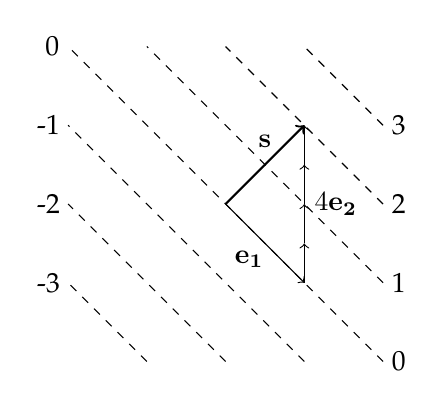
\begin{tikzpicture}
        \draw[dashed] (1,0) -- (0,1);
        \node at (-0.25,1) {-3};
        \draw[dashed] (2,0) -- (0,2);
        \node at (-0.25,2) {-2};
        \draw[dashed] (3,0) -- (0,3);
        \node at (-0.25,3) {-1};
        \draw[dashed] (4,0) -- (0,4);
        \node at (-0.2,4) {0};
        \node at (4.2,0) {0};
        \draw[dashed] (4,1) -- (1,4);
        \node at (4.2,1) {1};
        \draw[dashed] (4,2) -- (2,4);
        \node at (4.2,2) {2};
        \draw[dashed] (4,3) -- (3,4);
        \node at (4.2,3) {3};
        \draw[thick,->] (2,2) -- (3,3);
        \node at (2.5,2.8) {$\vec{s}$};
        \draw[thin,->] (2,2) -- (3,1);
        \node at (2.3,1.3) {$\vec{e_1}$};
        \draw[thin,->] (3,1) -- (3,1.5);
        \draw[thin,->] (3,1.5) -- (3,2);
        \draw[thin,->] (3,2) -- (3,2.5);
        \draw[thin,->] (3,2.5) -- (3,3);
        \node at (3.4,2) {$4\vec{e_2}$};
    \end{tikzpicture}
    \label{fig:gradient-vector-awk}
\end{figure}

For absolute clarity we've spelled out the scaling and addition of the basis vectors, to show that $\vec{s}$ is equivalent to adding $4$ lots of $\vec{e}_2$ on to the end of $\vec{e}_1$, just as the coordinates of $\vec{s}$ tell us to do. But the key point is that this is physically the same vector we found when working in the standard orthonormal basis (Figure \ref{fig:gradient-vector}). It is described by different coordinates, of course, but it's the same vector, pointing in the direction of steepest increase. It even has the same magnitude $\|\vec{s}\|$, which is the square root of the inner product of $\vec{s}$ with itself. The inner product will use the lowering metric to convert one of those $\vec{s}$ inputs to $\vec{d}$ so it can act on the other $\vec{s}$, ensuring a consistent result.

Similarly, given $\vec{s}$ and some other vector $\vec{x}$ representing a displacement, we can directly obtain the change in $T$ due to that displacement using the inner product $(\vec{s}, \vec{x})$ between them:

\begin{equation}
\begin{split}
dT &= (\vec{s}, \vec{x}) \\
   &= \sum_{\nu} \left( \sum_{\mu} g_{\mu\nu} s^{\mu} \right) x^{\nu} \\
    &= \sum_{\nu} d_{\nu} x^{\nu}
\end{split}
\end{equation}

\subsection{Smoothly varying gradients}

Generalising this to the more complicated kinds of $T$ scalar field, the scalar-valued function $dT(\vec{x})$, that tells us how $T$ changes due to a small displacement $\vec{x}$, may have a different definition at each point in space. But we can retain the simplification that we only need to know the linear approximation of that function at each point.

The displacement will be described by a number in each dimension: a relative coordinate change associated with each position basis vector. If we only allow one coordinate, $x^i$, to vary and leave the others constant, $dT$ becomes a scalar-valued function of a single variable, $x^i$, which if plotted would simply be a line through the origin (i.e. it is $0$ when its parameter is $0$). It is therefore characterised entirely by a single number, its gradient, the number by which it multiplies its input.

The function $T$ is of course not necessarily linear in $x^i$. Following the Maclaurin method (§\ref{sec:unit-circle-maclaurin}), we assume that whatever the function is, it can be expressed as a polynomial series\footnote{Warning! In this context we're dealing with scalar variables and $x^n$ briefly means "$x$ to the power of $n$", not the $n$th component of $\vec{x}$.} of the form $d_n x^n$. The first term ($n = 0$, $x^0 = 1$) is just a constant: the value of $T$ at the current position. We will be subtracting this from the total, because we want to know how $T$ changes as we move away from that position. The terms $n > 1$ involve $x^2$, $x^3$ and so on. As $x$ becomes arbitrarily small, these terms plummet in significance very rapidly. So that leaves just the term $d_1 x$, and $d_1$ is the only number we need to describe the tangent line to the curve of the function at the current position. We can therefore discard its subscript label, and replace it with $i$, as it's the sole outcome of this analysis when varying the $i$th component of $\vec{x}$:

$$
\frac{\partial T(\vec{x})}{\partial x^i} = d_i
$$

We carry out this analysis $i$ times to get the linear gradient number for all $i$ components, and thanks to linearity we can simply add them to get the total change in $F$:

$$
d T(\vec{x}) = \sum_i \frac{\partial T(\vec{x})}{\partial x^i}
= \sum_i d_i x^i
= \langle \vec{d} , \vec{x} \rangle
$$

Once again it's just the covector $\vec{d}$ described by coordinates $d_i$, acting on the displacement vector $\vec{x}$ described by coordinates $x^i$. Then to obtain the components of the gradient vector, which is the dual of $d$, we apply the raising metric $g^{\mu\nu}$ to $d$.

The trivial example of the linear field with constant gradient $T(\vec{x}) = x^1 + x^2$ was therefore in fact fully illustrative, because if the function had any terms that weren't linear, we would have just ignored them anyway.

The way this is usually described, the operator that obtains the field of gradient vectors (the $\vec{s}$ associated with each point in space) from a field of scalars $T(\vec{p})$ is $\nabla T(\vec{p})$, the $\nabla$ being pronounced "del". This is very often conflated with the \textit{total derivative}, which is the somewhat confusing name for the covector $\vec{d}$ associated with each point in space. The reason they are often casually conflated is because if the basis vectors are orthonormal then they have the same coordinates. A careful author will be clear about this requirement when claiming that "the dot product" (rather than the properly defined inner product) can be used to get the \textit{directional derivative} from the gradient vector and the unit vector in the direction of interest.

\subsection{Sources of confusion}

A major potential source of confusion in this area is the distinction between the total derivative, a covector, and the gradient, a vector, and how and why they might be affected by a change of basis. As we've seen, they are \textit{not} affected by a change of basis. Vectors and covectors never are. Their coordinates are affected, of course.

Another source of confusion is the way we think of the gradient as the rate of change of the scalar field, computed with respect to a change in position. This means that a physical distance appears on the bottom of a fraction, and therefore if we increase the size of our unit of distance, the number on the bottom of the fraction decreases, which increases the overall value of the fraction. This reminds us of covariance; is this the source of some inherently covector-like nature in gradients? No. As we've seen, the gradient is actually a vector, and so its coordinates transform contravariantly. The total derivative is a covector that maps a displacement vector to a change in the scalar field, so its coordinates transform covariantly. These two representations actually convey the same information (even in the form of the same set of numbers if the basis is orthonormal), so there is nothing inherently covariant about that information.

\chapter{Potentials} \label{ch:potential}

A force field is a vector-valued function of space, i.e. at each point in space we imagine there is a vector giving the strength and direction of the force that would felt at that point.

The force fields we observe in nature have an interesting property: it is always possible to replace the force field with a scalar-valued function of space, i.e. at each point in space there is merely an ordinary number, not a vector. We can then take the vector gradient $\nabla$ of this scalar field and we recover the force field.

By analogy, picture a hilly landscape. The height $H$ above sea level is the scalar field value, so the landscape is fully described by the scalar field $H(x, y)$. From this we can derive $\nabla H$, a two-dimensional vector field (picture it as an arrow that never points up or down, always parallel to the horizon). As we travel around we sometimes face steep slopes, where $\nabla H$ points in the steepest direction, or stationary points such as hilltops or valley basins where $\nabla H$ is the zero vector (to distinguish between peaks and valleys, we'd need to take the second derivative, $\nabla^2H$).

If we wander on some pathway through this landscape and return back to where we started, our height will be the same as it was when we started (assuming the landscape hasn't changed shape). This is true regardless of the path we take, as the height is a fact about the start/end point of the path. This is so obvious as to seem hardly worth stating.

And yet if we only had some vector field, and wondered if the path integral of any closed loop through that field was always zero, how would we know? Some paths might go mainly through regions with vectors all pointing in one direction, and so not sum to zero. Not all vector fields have this self-balancing property.

Those that do are known as conservative fields, and these are fields which can be reduced to a scalar field from which the vectors can be recovered by applying $\nabla$, and these are all the force fields we encounter in nature.

When we describe a force field by a scalar field, we call that field a \textit{potential}. It has units of energy. As a particle moves through a potential, it experiences a potential difference between two points. If this difference is negative, i.e. the potential energy drops between the two points, the particle gains kinetic energy (speeds up). This is exactly like a ball rolling down a slope; the potential energy is exactly equivalent to the height of the landscape.

If the potential does not vary, the gradient is zero. This is true regardless of the potential's constant value, which is like a constant of integration, i.e. a global increase in potential is physically meaningless.

An important example is a force field conforming to the inverse square law, so the force is proportional to $r^{-2}$ where $r$ is the distance from the origin of the force. The potential must therefore be proportional to $r^{-1}$, so that it has the required gradient (differentiation subtracts 1 from the power of a polynomial).

\section{Complex vector spaces}\label{sec:vectors-complex}

We've mentioned that a vector space has an associated set of scalars, and this is often $\mathbb{R}$, but it may instead be $\mathbb{C}$, meaning that vectors can be scaled by a complex number, and if expressed as a column of coordinates, those coordinates may be complex.

Even the simplest non-trivial example of such a space, $\mathbb{C}^2$, is not directly imaginable, because although each vector requires two coordinates, each of those is a complex number incorporating a real and imaginary part, so each vector requires four real numbers to describe it, and so $\mathbb{C}^2$ is isomorphic with $\mathbb{R}^4$, which is impossible to visualise directly.

Even so, concepts applicable to real vector spaces also work for complex, although with some modifications. The main issue is determining the modulus, for which we must introduce an inner product.

If we use the usual dot product definition then we have a problem because we naturally expect the modulus to be a positive real number. Summing the squares of the components of a complex vector could well produce a negative result, and then we need to take the square root to get the modulus, so the modulus wouldn't even be a real number.

To ensure $\langle \vec{u}, \vec{v} \rangle$ is real and positive, we amend the inner product so that we first take the complex conjugate of one its arguments:

$$
\langle \vec{u}, \vec{v} \rangle
=
\vec{u}^* \cdot \vec{v}
$$

This has the complicating side-effect that commutativity:

$$
\langle \vec{u}, \vec{v} \rangle
=
\langle \vec{v}, \vec{u} \rangle
$$

no longer applies. But who says it needs to? We instead make the requirement be:

$$
\langle \vec{u}, \vec{v} \rangle
=
\left[ \langle \vec{v}, \vec{u} \rangle \right]^*
$$

This is sometimes called conjugate symmetry. If all the components are real then complex conjugation makes no difference and commutativity is restored, so the nice thing is that we've amended the rule in a way that is "backward compatible" with real vectors.

This does mean that when taking the inner product of two different complex vectors, it matters which one we take the complex conjugate of. In physics the convention is to take the conjugate of the LHS vector.

The general form of the inner product, where we supply a matrix to control how to pair up and weight the coordinates, is similarly amended.

We use the dagger $^\dagger$ symbol to mean conjugate transpose, where we transpose a matrix (so turn a column vector into a row) and also take the complex conjugate of every element. It's equivalent to applying both $^\intercal$ and $^*$.

$$
\langle \vec{u}, \vec{v} \rangle
=
u^\dagger \mathbf{M} v
$$

As usual if $\mathbf{M}$ is $\delta$ then this reduces to the first definition given above. It should at least be be self-adjoint or Hermitian, which is to say that:

$$\mathbf{M}^\dagger = \mathbf{M}$$

That is, every element is the complex conjugate of its diagonally opposing element, and that therefore elements on the diagonal are real (they aren't moved by the transposition and so must equal their own complex conjugates).

A matrix like this is the complex equivalent of the real symmetric matrix for which we gave a definition (§\ref{ch:vectors-symmetric}).

Several other important facts about Hermitian operators can be derived: their eigenvalues are all real, their eigenvectors are orthogonal and span the space and so can be used to construct an orthonormal basis.

Another interesting kind of operator in complex spaces is those where:

$$\mathbf{U}^\dagger \mathbf{U} = I$$

i.e. the identity operator. These are known as unitary operators. They have the property of preserving the inner product (is the same property we observed before for rotations and mirrorings):

$$\langle \vec{u}, \vec{v} \rangle = \langle \mathbf{U} \vec{u}, \mathbf{U} \vec{v} \rangle$$

If you have a Hermitian operator expressed by the matrix $M$ you can convert it to another representation by wrapping it in a transformation $T$ and its inverse:

$$M' = T M T^{-1}$$

If $T$ is unitary then $M'$ will be Hermitian, recognisable by the relationship between diagonally opposite matrix elements.
\chapter{Quantum Mechanics} \label{ch:qm}

\section{State Vectors and Dirac Notation}

In quantum mechanics everything knowable about the state of some system is described in a vector, known as the state vector. The vector is from a vector space defined over the field of complex numbers, so it is important to use the correct definition of the inner product (\ref{ch:vectors-complex}) where we take the conjugate of one of the vectors, to ensure that the inner product of a vector with itself is a non-negative a real number.

The inner product in this context is written like this:

$$\langle a|b \rangle$$

If the vectors $\vec{a}$ and $\vec{b}$ are represented by column matrices $a$ and $b$, the above is equivalent to conjugate-transpose of $a$, written as $a^{\dagger}$ ("a-dagger"), matrix-multiplied by $b$:

$$a^{\dagger} \, b$$

We can split this inner product notation into separate pieces, so we can write $\langle a|$ to mean the vector whose matrix representation in some basis is a single row containing the complex conjugates of the elements in the single column of the matrix representing $|a \rangle$ in the corresponding dual basis.

Or more simply, $\langle a|$ is the covector of $|a \rangle$. The convention is therefore to think of $\langle a|$ as an operator that extracts the coordinate of a basis vector $|a \rangle$ from its argument, which will be some vector $|b \rangle$, as in the expression $\langle a|b \rangle$.

\section{Hilbert Spaces}

The vector spaces used to represent physical states are examples of Hilbert spaces, which for our purposes means that:

\begin{itemize}
  \item they have an inner product that we can use to get a non-negative real number for the modulus of a vector: $\sqrt{\langle a|a \rangle}$, and 
  \item they may be infinite dimensional.
\end{itemize}

The latter possibility includes infinities that are continuous (uncountable). Such vectors cannot be represented by a column of discrete values. Instead we have to specify a complex-valued function over a continuous (real) variable. Such functions can be added and scaled, as is required of a vector (\ref{ch:linearity}) and so they qualify as elements of a vector space (\ref{sec:vectors-space}) and we therefore have no choice but to admit that they are vectors.

The real value is analogous to the integer index that labels the rows in a column vector; instead of fetching the $i$th component by its position in the column, we evaluate the function with some real value $x$.

Similarly, where as the inner product over discrete components is:

$$
\langle a | b \rangle
=
\sum_i
x_i^* y_i
$$

the inner product over functions $f$ and $g$ of a real variable $x$ is:

$$
\langle f | g \rangle
=
\int_{-\infty}^{+\infty}
f(x)^* g(x)
dx
$$

Thus we can in some sense find the square of the "length" of a function: $\langle f | f \rangle$.

\section{Physical Interpretation}

To interpret the state vector physically, we choose a basis so we can resolve it into components. Our choice of basis has to do with the observable quantity we are presently interested in, such as position, momentum or energy. If it may take on any real value, the state vector will have to be a function of that value; if it may only take on certain discrete values, it can be a column vector (albeit sometimes one with infinitely many rows) in which each row corresponds to one of those possible discrete values that the observable may exhibit when measured.

The information available from the state vector is, in general, probabilistic. Each component, being a complex number, is related to the probability of the observable quantity taking on the value represented by that component. The modulus of the component (its value multiplied by the complex conjugate of its value) is the probability of obtaining that value, or if the state vector is a function $f(x)$, then:

$$\int_{a}^{b} f(x)^* f(x) \, dx$$

is the probability that $x$ will have a value somewhere between $a$ and $b$.

As a probability is a number between 0 and 1, it must be the case that the sum of all the components (or the above integral from $-\infty$ to $+\infty$) must be $1$. This is the same as saying that $\langle S | S \rangle = 1$ for any physically realistic state vector. Or to put it another way, the magnitude of a state vector is not significant, only the direction (i.e. the relative values of the components in some basis). We will always fix the magnitude to be $1$.

Unsurprisingly, if one of the components is $1$ and all the others are zero, the vector represents certainty that the observable has the value represented by that components. But this also means that the state vector is equal to one of the basis vectors. Thus the basis vectors represent exact values that the observable may exhibit when measured.

Further, a measurement of the observable (or more precisely, any interaction producing subsequent behaviour that could be used to infer the value of the observable) causes the state vector to change to a basis vector of that observable, the likelihood of each possible state determined by previous state vector's component for that state's basis vector. This change is (at least in this theory) assumed to be instantaneous and to have no mechanism that we can deduce anything further about.

Thus after measuring an observable, subsequent measurements of the same observable will with certainty produce the same result.

(This is not quite true in the continuous cases when the state vector is actually a function of a real variable. We don't expect to ever find such a system precisely aligned with a single base state, but instead to have at least some small spread of probabilities.)

\section{Switching Basis}

Having constructed a column representation of a state vector in one basis, relating to one observable, we can switch to another using an operator ()\ref{sec:vectors-change-basis}). A state vector contains everything knowable about a system, including all we can know about any of its observable quantities. To switch observables means to switch basis, re-expressing the same state vector as a different set of components against the new basis.

As always when using a matrix to transform a vector's components we need to be clear on whether we want to get a different vector in the same basis or the same vector in a different basis. In this case, physically we're talking about the latter; a state vector represents something physically real, and we're just changing how we describe it. On the other hand, mathematically all we have is the description, and the choice of basis is not entirely arbitrary because a basis relates to an observable quantity.

The operator for selecting another observable is Hermitian or self-adjoint, meaning that for an operator $\hat{O}$:

$$\langle a|\hat{O} b \rangle = \langle \hat{O} a| b \rangle$$

This has a few useful implications:

\begin{itemize}
  \item in the discrete finite vector case, they can be represented as a matrix $O$, $O^{\dagger} = O$, or $O_{ij} = O_{ji}^*$, so the main diagonal elements are real,
  \item regardless of representation, their eigenvectors (\ref{sec:vectors-eigen}) are orthogonal and complete (they span the space, so you can take a unit vector in each of these orthogonal directions and you have an orthonormal basis) and
  \item regardless of representation, their eigenvalues are real.
\end{itemize}

Think of the analogy of a Euclidean real plane vector space, and a symmetric $2 \times 2$ matrix $M$ operating on it. The eigenvectors are lines in the plane along which vectors do not change direction, only magnitude, when the operator is applied. Because the matrix is symmetric ($M_{ij} = M_{ji}$) these lines are orthogonal. So it is with a Hermitian operator in a complex space, with only the added complication of needing to be careful about taking the complex conjugate when comparing diagonally opposite elements.

The basis vectors of the new observable are just unit vectors that are eigenvectors of the operator. So in the old basis (that is, the old observable) the state vector may have represented a degree of uncertainty, not being aligned with any one basis vector of that basis, but in the new basis it may happen to be aligned precisely with a basis vector and thus represent certainty that a specific value will be measured. More likely we will have prepared a system in a known state, so its state vector very nearly equal to some basis vector of the initial basis, and we want the probability distribution for another observable, so we'll convert to that observable's basis.

If $|b \rangle$ is the prepared state of the system, and $\hat{O}$ is the observable we want to know the probability distribution for, and in particular we're interested in the probability amplitude of a particular measurement outcome of $\hat{O}$ represented by the basis vector $|a \rangle$, then:

$$
\langle a | \hat{O} |b \rangle
$$

The eigenvalues that go with each eigenvector are also significant: they are the physical measured values that the observable make take on.

So the $i$th component of the new representation of the state vector relates to the $i$th observable value (given by the eigenvalue) and is the coefficient of the basis vector $|i \rangle$, which is a unit vector that is an eigenvector corresponding to the $i$th eigenvalue.

Of course, all operators for transitioning to other bases must also be updated so they work from the new basis. For example, to get back to the previous basis we would need to do the inverse transformation.

While we've discussed all this in terms of more easily pictured finite-dimensional vectors with discrete complex components, all the same concepts translate to complex-valued functions of an integer or real parameter.

\section{The Wave Function}

One way to approach QM initially is to consider the position and momentum of an electron. These are continuous variables, so we will be working entirely with state vectors that are represented by functions of real variables, and operators that transform functions.

We model this situation as a continuous complex-valued function of position and time, $\Psi(x, y, z, t)$, very often abbreviated to $\Psi$. We will sometimes also consider functions only of space, $\psi$. (This upper/lowercase distinction is quite widespread but not universally observed.)

By considering only one spatial dimension we can picture the wave function at one instant as a line, somewhere along which the electron could be found. At each point $x$ on the line there is an associated complex plane (visualised as normal to the line), with an arrow lying in it, pointing out from the line. This is the complex value of $\Psi$ at that position $x$ and time $t$.

This complex plane should not be confused with vectors. Any given snapshot of $Psi$ at some instant $t$, given by a function $\psi(x)$, is itself an entire vector. The position $x$ labels a single infinitesimal component of the vector, and every such component is a complex number, which we can therefore visualise as a complex plane with an arrow on it.

So for example we could picture the arrows as making a corkscrew shape, rotating around the line such that the angle depends linearly on $x$, but the modulus of the complex value (the length of the arrow) happens to be constant in this example. This is the notional wave function for a free electron (no forces acting it) with a precisely defined momentum and therefore no defined position.

More generally, the arrow length will also vary with $x, t$. The arrow length at $x$ determines the likelihood that the electron will be found at $x$. More precisely, the modulus-squared of $\Psi$, which can be calculated with $\Psi^*\Psi$, is proportional to the probability density:

$$\rho(x) = \Psi^*\Psi$$

Given the electron is in some region $A$ between $x_1$ and $x_2$, the integral:

$$
\alpha =
\int_{x_1}^{x_2}
\Psi^*\Psi
\,dx
$$

is \textit{proportional} to the probability of finding the electron in $A$.

Recall that the product of a complex number and its own complex conjugate is a real number, and here we are doing $\Psi(x)^*\Psi(x)$, using the single complex value at position $x$, so the result will be real. But the complex conjugate is not a general purpose magic way to get a real number from a product of any two complex numbers; $\Psi(x_1)^*\Psi(x_2)$ need not be real.

If we compute the same integral $\beta$ for some larger surrounding region $B$, we can compute the conditional probability:

$$
P(A|B) = \frac{\alpha}{\beta}
$$

That is: the probability of finding the electron in $A$ \textit{given that} it is somewhere in $B$ is given by the fraction $\alpha / \beta$.

If $\Psi$ is suitably behaved (square-integrable; roughly, it goes to zero at some distance and does not become infinite anywhere) then we can compute the integral over the whole of our one dimension of space:

$$
\alpha =
\int_{-\infty}^{+\infty}
\Psi^*\Psi
\,dx
$$

We can then include a factor of $1/\sqrt{\alpha}$ within $\Psi$ to "normalise" it, such that integrating the normalised $\Psi^*\Psi$ over some region will directly give us the absolute (unconditional) probability of finding the electron in that region.

Some interesting things to note at this early stage:

\begin{itemize}
  \item For the simple first example of the free electron with definite momentum, normalisation is not possible because the integral over all of space does not converge on a finite value.
  \item A global change in the amplitude of the function (scaling the entire function by some complex constant) is not a physically significant change; there is a set of wave functions $a\Psi$ for any complex constant $a$, which all mean the same thing. What matters is how the amplitude varies from place to place (the same will turn out to be true for the complex phase).
\end{itemize}

\section{Schrödinger Equation}

Any wave can be described as a sum of many simple component waves. Each individual component wave has \textit{two} parameters:

\begin{itemize}
  \item if we nominate a fixed point in space, there is a frequency of oscillation, $\nu$
  \item if we freeze time, we can measure the wavelength, $\lambda$, the distance between adjacent peaks in space
\end{itemize}

These can be independently adjusted (do not be confused by the familiar example of EM waves, where wavelength and frequency are coupled due to the constant speed of light!)

So the component wave can be described by the complex exponential:

$$
\Psi(x, t) = \exp \left[ 2\pi i(\frac{x}{\lambda} - \nu t) \right]
$$

Pick any fixed point in space, so $x$ is constant, and $\nu$ determines the rate of oscillation. Pick a fixed instant in time, so $t$ is constant, and $\lambda$ determines the distance between peaks. With both in play, we have a corkscrew complex wave pattern that is moving.

Anything we figure out for this model wave can be taken to be true for any linear combination of many such waves, in the sense that we can imagine decomposing some messy wave into a set of components, each component characterised only by two numbers.

Planck inferred the relationship between frequency and energy:

$$\nu = \frac{E}{h}$$

And de Broglie likewise for momentum and wavelength:

$$\lambda = \frac{h}{p}$$

So we can write the wave function very neatly in terms of energy and momentum instead:

$$
\Psi(x, t) = \exp \left[ {\frac{i(px - Et)}{\hbar}} \right]
$$

Nothing much has changed: as before, we have two parameters shaping a complex corkscrew wave. (We use $\hbar = h/2\pi$ for brevity because that combination isn't going away.) All that has changed is that we've got two parameters with a physical interpretation for something we've previously thought of as a "particle".

We can take the partial differential of the above w.r.t $t$ or $x$, and the way that works with exponentials is strangely illuminating.

Doing $t$ first:

$$
\frac{\partial \Psi}{\partial t}
=
-\frac{iE}{\hbar}
\exp \left[ {\frac{i(px - Et)}{\hbar}} \right]
$$

The constant factor is copied outside the exponential, which otherwise remains the same. So in fact:

$$
\frac{\partial \Psi}{\partial t}
=
-\frac{iE}{\hbar}
\Psi
$$

We can tidy up by multiplying both sides by $i\hbar$:

$$
i\hbar \frac{\partial \Psi}{\partial t}
= E \Psi
$$

The exact same procedure with $x$ yields:

$$
- i\hbar \frac{\partial \Psi}{\partial x}
= p \Psi
$$

But we can also take the second derivative and get:

$$
- \hbar^2 \frac{\partial^2 \Psi}{\partial x^2}
= p^2 \Psi
$$

Returning to our physical interpretation, a free particle has energy that is purely kinetic, related to its momentum by:

$$
p^2 = 2m E
$$

(This is just $\frac{1}{2}mv^2$ smushed into the definition of momentum, $mv$.)

Substituting the Planck and de Broglie relations:

$$
\frac{\hbar}{2m} = \lambda^2\nu
$$

In general a corkscrew wave is governed by two independent parameters:

\begin{itemize}
  \item momentum, which goes with wavelength (and the $x$ coordinate)
  \item energy, which goes with frequency (and the $t$ coordinate)
\end{itemize}

We've now coupled them, making them no longer independent. But we've also added a new parameter: the particle's mass. For a free particle of a given mass, if you know the momentum you know the energy, and vice versa. Equivalently, if you know the wavelength you know the frequency, and vice versa.

Returning to the classical relationship between momentum, energy and mass, we can use it to rewrite our expression for $p^2 \Psi$, substituting into the R.H.S. to easily obtain:

$$
- \hbar^2 \frac{\partial^2 \Psi}{\partial x^2}
= 2mE\Psi
$$

And as we also have an expression for $E\Psi$, let's isolate that:

$$
E\Psi =
- \frac{\hbar^2}{2m} \frac{\partial^2 \Psi}{\partial x^2}
$$

and insert our $E\Psi$ expression:

$$
i\hbar \frac{\partial \Psi}{\partial t}
=
- \frac{\hbar^2}{2m} \frac{\partial^2 \Psi}{\partial x^2}
$$

So, recalling that $\Psi$ is an abbreviation for $\Psi(x, t)$, a complex valued function of space and time, now we have a differential equation that relates only these things:

\begin{itemize}
  \item $\hbar$, Planck's constant, a universal fixed real number with units of joules-seconds, very accurately determined by experiment, not something we can adjust to fit this equation to different scenarios
  \item $i$, which just provides a 90\textdegree phase shift
  \item the first partial derivative of $\Psi$ w.r.t. to time, which is another function of space and time that tells you how $\Psi$ is changing
  \item $m$, the mass of the particle
  \item the second partial derivative of $\Psi$ w.r.t. space.
\end{itemize}

This means that from a snapshot $\psi$ (at a specific instant of time) of the wave function of a particle with a known mass, so you have its shape in space, you can find the second derivative of that shape w.r.t. space, then multiply that by $i\hbar/2m$ and you have the the first partial derivative of $\Psi$ w.r.t. to time. That is, a snapshot contains complete information about the past and future of the wave; it tells you how to compute every past and future state.

So far, so kind-of rigorous. The situation becomes vaguer when we introduce a force field acting on the particle.

Schrödinger himself seems to have mostly taken a guess and found that the resulting equation agreed with several previously unexplained experimental results. Many widely used textbooks don't even give any background for it but merely state it. More advanced theory can be used to derive it, e.g. it is a low-energy approximation of QED.

The full classical account of the energy of a particle is:

$$
E = \frac{p^2}{2m} + V
$$

where the potential is a function $V(x)$. Realistically it will also be a function of $t$, but later we're going to pretend it isn't.

Some authors note that by multiplying the above throughout by $\Psi$:

$$
E\Psi = \frac{p^2{\Psi}}{2m} + V{\Psi}
$$

we obtain some scaffolding into which we can plug in our expressions for $E \Psi$ and $p^2 \Psi$:

\begin{equation}
i\hbar \frac{\partial \Psi}{\partial t}
=
- \frac{\hbar^2}{2m} \frac{\partial^2 \Psi}{\partial x^2}
+ V{\Psi}
\label{eqn:se}
\end{equation}

And this is the same as the free particle equation with the added $V\Psi$ term, and is the complete Schrödinger equation which governs the time evolution of $\Psi$.

The extra term doesn't change the important property that if you have a snapshot $\psi(x)$ taken of $\Psi(x, t)$ at a specific initial instant of time, then you know all future states (glossing over what happens when there is any kind of interaction, including measurements).

This is sometimes contrasted with Newton's 2nd law relating acceleration to force, acceleration being the second order derivative of the position w.r.t time. Each time we integrate we need to conjure up a constant of integration, and we have to integrate acceleration twice to get the position. The two constants we need to add are the position and velocity. Thus a snapshot of the position of a particle is not generally enough to know what is happening to it.

But a snapshot $\psi(x)$ taken of $\Psi(x, t)$ at some time is not just one number, but a continuous function giving a (complex) number at each point $x$ along the line, so it is generously endowed with information. If we decompose the snapshot into component waves, each one has its own wavelength.

And if we multiple $\Psi$ by some constant (possibly complex) factor, the result is still a solution to the function. Such arbitrary constant scale factors make no difference to the physical meaning; what matters is how the function varies from location to location (and from time to time). This is what allows us to normalise the function (where possible) to ensure that it sums to 1 over all of space.

\section{Time Evolution}

We can say little here about wave functions unless they can be normalised, i.e. wave functions that tend to zero at infinity. Assuming this is the case, if we integrate the PDF over all of space:

$$
\int_{-\infty}^{+\infty}
\Psi^*\Psi
\,dx
$$

we expect the result to be constant (if normalised, it should always remain 1 as time passes), i.e.

$$
\frac{d}{d t}
\int_{-\infty}^{+\infty}
\Psi^*\Psi
\,dx
= 0
$$

Note that as we are integrating over $x$, outside the integral $x$ is not a variable. We can move the differentiation w.r.t. $t$ inside the integral, but only we change it to partial, because inside the integral $x$ is a variable:

$$
\int_{-\infty}^{+\infty}
\frac{\partial}{\partial t}
\Psi^*\Psi
\,dx
= 0
$$

Focusing on the inside of the integral, by the product rule:

$$
\frac{\partial}{\partial t} \, \Psi^*\Psi
=
\frac{\partial \Psi^*}{\partial t} \Psi
+
\frac{\partial \Psi}{\partial t} \Psi^*
$$

Now, the Schrödinger equation gives us an expression for the partial time derivative of the wave function by slightly rearranging \eqref{eqn:se}:

$$
\frac{\partial \Psi}{\partial t}
=
\frac{i \hbar}{2m} \frac{\partial^2 \Psi}{\partial x^2}
- \frac{i V}{\hbar}{\Psi}
$$

From this we can get the same for the complex conjugate:

$$
\frac{\partial \Psi^*}{\partial t}
=
- \frac{i \hbar}{2m} \frac{\partial^2 \Psi^*}{\partial x^2}
+ \frac{i V}{\hbar}{\Psi^*}
$$

Plugging those into our expression:

$$
\frac{\partial}{\partial t} \, \Psi^*\Psi
=
\left[
- \frac{i \hbar}{2m} \frac{\partial^2 \Psi^*}{\partial x^2}
+ \frac{i V}{\hbar}\Psi^*
\right] \Psi
+
\left[
\frac{i \hbar}{2m} \frac{\partial^2 \Psi}{\partial x^2}
- \frac{i V}{\hbar}\Psi
\right] \Psi^*
$$

Multiplying out:

$$
\frac{\partial}{\partial t} \, \Psi^*\Psi
=
- \frac{i \hbar}{2m} \frac{\partial^2 \Psi^*}{\partial x^2}
\Psi
+ \frac{i V}{\hbar}\Psi^*\Psi
+
\frac{i \hbar}{2m} \frac{\partial^2 \Psi}{\partial x^2}
\Psi^*
- \frac{i V}{\hbar}\Psi\Psi^*
$$

The second and fourth terms cancel each other:

$$
\frac{\partial}{\partial t} \, \Psi^*\Psi
=
- \frac{i \hbar}{2m} \frac{\partial^2 \Psi^*}{\partial x^2}
\Psi
+
\frac{i \hbar}{2m} \frac{\partial^2 \Psi}{\partial x^2}
\Psi^*
$$

Also there's a common factor we can pull out:

$$
\frac{\partial}{\partial t} \, \Psi^*\Psi
=
\frac{i \hbar}{2m}
\left[
\frac{\partial^2 \Psi}{\partial x^2}\Psi^*
- \frac{\partial^2 \Psi^*}{\partial x^2}\Psi
\right]
$$

Recall that we are working out an expression for this because it appears inside an integral over all space:

$$
\int_{-\infty}^{+\infty}
\frac{i \hbar}{2m}
\left[
\frac{\partial^2 \Psi}{\partial x^2}\Psi^*
- \frac{\partial^2 \Psi^*}{\partial x^2}\Psi
\right]
dx
$$

Now the fundamental theorem of calculus is that integration is the inverse of differentiation, so there is clearly some redundancy here in that we are taking the second partial differential w.r.t. $x$ only to then integrate over all $x$.

To make this explicit:

\begin{equation}  
\frac{\partial}{\partial t} \, \Psi^*\Psi
=
\frac{i \hbar}{2m} \
\left[
\frac{\partial}{\partial x}
\left(
\frac{\partial \Psi}{\partial x}\Psi^*
- \frac{\partial \Psi^*}{\partial x}\Psi
\right)
\right]
\label{eqn:qm-byparts}
\end{equation}

The integral and the partial differentiation w.r.t. $x$ cancel out to give us an expression that we can evaluate at the two limits and take the difference:

$$
\frac{d}{d t}
\int_{-\infty}^{+\infty}
\Psi^*\Psi
\,dx
=
\frac{i \hbar}{2m}
\left[
\frac{\partial \Psi}{\partial x}\Psi^*
- \frac{\partial \Psi^*}{\partial x}\Psi
\right]
\bigg\rvert_{-\infty}^{+\infty}
$$

If we do that, we will have an expression for the rate of change, w.r.t. to time, of the integral of $\Psi^*\Psi$ over all space.

But at these limits, we've said $\Psi$ goes to zero, so as to be normalisable, making the whole expression zero at those limits. So in fact we've shown that, as we wanted:

$$
\frac{d}{d t}
\int_{-\infty}^{+\infty}
\Psi^*\Psi
\,dx
= 0
$$

So if it is possible to normalise a wave function at all, and it satisfies eqn. \ref{eqn:se}, then the constant of normalisation lives up to its name: it is the same for all time.

\section{Motion}

Given this abstract notion of an electron being entirely represented by a complex-valued function of position, how can we make sense of an electron moving?

Supposing the wave function is more concentrated in some region, it makes sense to compute the expectation value of the position variable:

$$
\langle x \rangle =
\int_{-\infty}^{+\infty}
x \, \rho(x)
\,dx
$$

Substituting our definition of $\rho$ from $(1)$:

$$
\langle x \rangle =
\int_{-\infty}^{+\infty}
x \, \Psi^*\Psi
\,dx
$$

remembering always that $\Psi$ is short for $\Psi(x, t)$, so $\langle x \rangle$ is also a function of $t$, and so this gives us a way of thinking about motion: the way the expectation value of the position changes with time.

$$
\frac{d}{dt} \langle x \rangle =
\frac{d}{dt}
\int_{-\infty}^{+\infty}
x \, \Psi^*\Psi
\,dx
$$

We can rearrange to move the derivative inside the integral, giving:

$$
\frac{d}{dt} \langle x \rangle =
\int_{-\infty}^{+\infty}
x \frac{\partial}{\partial t}
\, \Psi^*\Psi
\,dx
$$

Like before, it's the $t$-derivative of something that depends on $x$, inside the integral over $x$ we clarify that it is the partial derivative, and therefore $x$ is a constant for that derivative.

And borrowing from eqn. \ref{eqn:qm-byparts} we can rewrite this as:

$$
\frac{d}{dt} \langle x \rangle =
\frac{i \hbar}{2m}
\int_{-\infty}^{+\infty}
x
\frac{\partial}{\partial x} \
\left(
\frac{\partial \Psi}{\partial x}\Psi^*
- \frac{\partial \Psi^*}{\partial x}\Psi
\right)
\,dx
$$

This isn't as simple as before where we cancelled out the integration and the differentiation, because of the pesky $x$. But the good news is this is the easiest ever opportunity for integration by parts. Recall:

$$
\int
u
\frac{dv}{dx}
dx = uv -
\int
v
\frac{du}{dx}
dx
$$

So $u$ is just $x$ and to get $v$ we have to calculate it at the limits:

$$
v =
\frac{\partial \Psi}{\partial x}\Psi^*
- \frac{\partial \Psi^*}{\partial x}\Psi
\bigg\rvert_{-\infty}^{+\infty}
$$

Plugging them in:

$$
x
\left(
\frac{\partial \Psi}{\partial x}\Psi^*
- \frac{\partial \Psi^*}{\partial x}\Psi
\right)
\bigg\rvert_{-\infty}^{+\infty}
-
\int_{-\infty}^{+\infty}
\left(
\frac{\partial \Psi}{\partial x}\Psi^*
- \frac{\partial \Psi^*}{\partial x}\Psi
\right)
\frac{dx}{dx}
dx
$$

As before, with $\Psi$ vanishing at infinity the first term can be removed, and of course $dx/dx$ is $1$. Finally the above is just the integral from our $\langle x \rangle$ expression, so:

$$
\frac{d}{dt} \langle x \rangle = -
\frac{i \hbar}{2m}
\int_{-\infty}^{+\infty}
\left(
\frac{\partial \Psi}{\partial x}\Psi^*
- \frac{\partial \Psi^*}{\partial x}\Psi
\right)
dx
$$

Having unwrapped one layer with integration by parts we can pull the same trick with $\frac{\partial \Psi^*}{\partial x}\Psi$, with $u = \Psi$ and $v = \Psi^*$, which once again means the $uv$ term is zero, leaving:

$$
-
\int_{-\infty}^{+\infty}
\frac{\partial \Psi}{\partial x}
\Psi^*
$$

So putting this back into $\langle x \rangle$:

$$
\frac{d}{dt} \langle x \rangle = -
\frac{i \hbar}{2m}
\int_{-\infty}^{+\infty}
\left(
\frac{\partial \Psi}{\partial x}\Psi^*
+ \frac{\partial \Psi}{\partial x}\Psi^*
\right)
dx
$$

The double minus means we're adding two identical terms, so:

$$
\frac{d}{dt} \langle x \rangle = -
\frac{i \hbar}{m}
\int_{-\infty}^{+\infty}
\frac{\partial \Psi}{\partial x}\Psi^*
dx
$$

If we think of the rate of change of $\langle x \rangle$ as the expectation value of the velocity, or $\langle v \rangle$, we can multiply by $m$ to get $\langle p \rangle$, which actually cancels the $m$.

$$
\langle p \rangle = -
i \hbar
\int_{-\infty}^{+\infty}
\frac{\partial \Psi}{\partial x}\Psi^*
dx
$$

\section{Operators} \label{sec:qm-operators}

Another way to look at what we're doing here is discovering operators. To apply an operator $\hat{O}$ and get its expectation value $\langle O \rangle$, the recipe is:

$$
\langle O \rangle =
\int_{-\infty}^{+\infty}
\Psi^*
\hat{O}
\Psi
\,dx
$$

Because $\Psi$ is a function of $x$ and $t$, by integrating over all $x$ we get a function of time, telling us the expectation value of whatever observable the operator represents.

To use this "operator sandwich" pattern, we just need to define our operators, and so far we have two.

The position operator $\hat{x}$ is just $x$ itself:

$$
\langle x \rangle =
\int_{-\infty}^{+\infty}
\Psi^*
\hat{x}
\Psi
\,dx
=
\int_{-\infty}^{+\infty}
\Psi^*
x
\Psi
\,dx
$$

The momentum operator $\hat{p}$ is $-ih\frac{\partial}{\partial x}$:

$$
\langle p \rangle =
\int_{-\infty}^{+\infty}
\Psi^*
\hat{p}
\Psi
\,dx
=
\int_{-\infty}^{+\infty}
\Psi^*
(-ih\frac{\partial}{\partial x})
\Psi
\,dx
$$

In fact all other observable quantities are represented by operators that can be defined in terms of $\hat{x}$ and $\hat{p}$.

\section{Time Independent Potentials}

In the Schrödinger equation, if the potential $V$ is constant everywhere (and thus may as well be zero everywhere), it reduces to the free particle equation that fell out automatically from the fact that kinetic energy is tied to momentum. If you know the energy, you know the momentum and vice versa, which means that if you know the shape of a time-independent snapshot of the wave $\psi(x)$, then you know everything.

If the potential is a function it gets trickier. To understand the effect of varying $t$ and $x$ separately, we can suppose the existence of two functions $\psi(x)$ and $\phi(t)$ that when multiplied gives us $\Psi(x, t)$.

It is not generally true that this is possible. Even something as simple as $\Psi(x, t) = x + t$ can't separated. It's obviously true that solutions to the zero-potential Schrödinger equation can be separated, simply because we obtained it from the assumption:

$$
\Psi(x, t) = \exp \left[ {\frac{i(px - Et)}{\hbar}} \right]
$$

which can easily be written as the product of two separate functions of $x$ and $t$:

$$
= \exp \left[ {\frac{ipx}{\hbar}} \right]
\exp \left[ {\frac{-iEt}{\hbar}} \right]
$$

But when a potential is included it transpires that we can only use separation of variables if the potential is only a function of $x$, not $t$.

We want to consider a wider range of functions, so will only assume:

$$\Psi(x, t) = \psi(x) \phi(t)$$

Taking partials becomes ordinary differentiation, because the other factor is constant:

$$
\frac{\partial \Psi}{\partial t}
= \psi \frac{d \phi}{d t},
\frac{\partial^2 \Psi}{\partial x^2}
= \frac{d^2 \psi}{d x^2}  \phi
$$

So we just plug those into eqn. \ref{eqn:se}:

$$
i\hbar
\psi \frac{d \phi}{d t}
=
- \frac{\hbar^2}{2m}
\frac{d^2 \psi}{d x^2}  \phi
+ V \psi \phi
$$

Dividing by $\psi \phi$:

$$
i\hbar
\frac{1}{\phi}
\frac{d \phi}{d t}
=
- \frac{\hbar^2}{2m}
\frac{d^2 \psi}{d x^2}
\frac{1}{\psi}
+ V
$$

To make this explicit, let's put the parameters on each function:

$$
i\hbar
\frac{1}{\phi(t)}
\frac{d \phi(t)}{d t}
=
- \frac{\hbar^2}{2m}
\frac{d^2 \psi(x)}{d x^2}
\frac{1}{\psi(x)}
+ V(x)
$$

The LHS only depends on $t$, the RHS only depends on $x$. This means if we hold $x$ constant, and therefore the RHS constant, this equation still holds even if we vary $t$! And of course vice versa. Which means both sides are equal to the same constant, and this is going turn out to be the energy $E$ as follows. Equating the LHS with $E$:

$$
i\hbar
\frac{1}{\phi}
\frac{d \phi}{d t}
= E
\implies
\frac{d \phi}{d t}
=
- \frac{Ei}{\hbar}
\phi
\implies
\phi = e^{-iEt/\hbar}
$$

The RHS isn't so neat, but:

$$
- \frac{\hbar^2}{2m}
\frac{1}{\psi}
\frac{d^2 \psi}{d x^2}
+ V
=
E
\implies
- \frac{\hbar^2}{2m}
\frac{d^2 \psi}{d x^2}
+ V\psi
=
E\psi
$$

Solutions for $\psi$ will depend on $V$ of course. But the whole wave function is therefore:

$$\Psi(x, t) = \psi(x) e^{-iEt/\hbar}$$

Why is this interesting? Because the more complicated space-sensitive part is frozen w.r.t. time, we can understand the time evolution by just looking at the extremely simple factor:

$$
e^{-iEt/\hbar}
$$

Whatever the solution to $\psi$, the complex value of every point in space is only changing by the above factor as time passes.

And that factor is really just $e^{i\theta}$ with the angle being $-Et/\hbar$, so we know the modulus of the value isn't changing; it's just going "round and round" clockwise in the complex plane.

And if the modulus isn't changing, the probability density isn't changing, so the particle isn't moving. Hence solutions of this type are known as \textit{stationary states}. The expectation value of the position is fixed, and so all other observables' expectation values are also constant, including energy.

Speaking of which, the total energy expectation value (kinetic plus potential) is:

$$
\hat{H} =
-\frac{\hbar^2}{2m}
\frac{\partial^2}{\partial x^2}
+ V(x)
$$

Comparing this to our RHS differential equation:

$$
- \frac{\hbar^2}{2m}
\frac{d^2 \psi}{d x^2}
+ V\psi
=
E\psi
$$

So it's just:

$$
\hat{H}\psi
=
E\psi
$$

Which tells us that our constant $E$ is indeed the total energy: a properly normalised $\psi$ integrated over all space is $1$, so multiplying it by a constant gets you the definite value $E$, and that's the expectation value of the total energy operator $\bar{H}$.

The above is in fact an eigenvalue equation: for some solutions $\psi$, the $\bar{H}$ operator has the same effect as multiplying by a constant, the eigenvalue $E$ for that $psi$. This exactly fits the vector-based framework for quantum mechanics that we began with.

All this is only true for the stationary states of separable $\Psi(x, t)$ wave functions, but we can add an infinite set of them to get other shapes:

$$
\Psi(x, t)
=
\sum_{n=1}^\infty
c_n
\psi_n
e^{-iE_nt/\hbar}
$$

So for each $n$ there's a complex constant $c_n$ to go with the stationary state $\psi_n$ and an energy level $E_n$ that controls how fast the global phase shift goes round and round.

Because we're adding complex values at each point in space, even though those component values each have a time-independent modulus, the sum of them does not. So this is a way to make non-stationary solutions. Wave packets that "move" can be composed by summing stationary states that do not.

\section{Wave Functions as Vectors}

For stationary states $m$ and $n$:

$$
\int
\psi_m^* \psi_n dx = \delta_{nm}
$$

This does not mean that $\psi_m^* \psi_n$ is zero everywhere if $m \ne n$, but it does mean that for every non-zero value pointing in some direction in the complex plane, there's another value of the same modulus pointing the opposite way, to balance it out.

The above is a way of defining the inner product between two stationary states, and of showing that they are like orthogonal vectors in a complex vector space for that product.

In fact we can define our vector space for QM in two ways:

\begin{itemize}
  \item as an uncountable continuum of \textit{scattering states}
  \item As a countable infinity of \textit{bound states}
\end{itemize}

\subsection{Scattering States}

In the uncountable case of scattering states, the vector is a function of a continuous coordinate and cannot be reduced to anything more compact than that. This happens when the potential is absent and we have a physical state that moves freely through space as a pulse waveform. The inner product is defined by an integral:

$$
\langle \alpha | \beta \rangle
=
\int
\alpha^* \beta \,dx
$$

If we knew a particle's exact location, $\alpha$, our wave function of space $\psi(x)$ would have a single spike where $x = \alpha$ and be zero everywhere else. Alternatively if knew its exact momentum (and $p=h/\lambda$) our wave function would be a wave with a single wavelength. So we're dealing with Fourier transforms. At these extremes of certainty/uncertainty, one domain has a simple wave of infinite extent, and the other domain has a spike representing that wave. It works either way round.

Thus far we've been working in "position space", using functions of $x$, but alternatively we could work in "momentum space", where the functions are $\phi(p)$. If we knew a particle's exact momentum, $\phi(p)$ would be a spike, whereas if we knew its exact position, $\phi(p)$ would be a single-component wave.

Either way, the point is that the elements of our vector space are functions of a continuous variable (a real number), and the inner product has to be an integral over that continuous variable.

\subsection{Bound States}

In the countable case of bound states, a potential traps a particle and the measurable energies are quantised, the energy being the eigenvalue of the energy operator applied to the stationary state eigenfunction at that energy level.

The energy eigenfunctions serve as a set of basis vectors, and we can create a weighted sum of them to make any state. We can use those weightings as the components of a vector describing a state. That is, the state of the lowest energy level is a column vector of numbers where the first component is $1$ and all the other components are $0$.

The inner product of two vectors is the sum of the products of the components of the two vectors (taking care to always complex conjugate the first one):

$$
\langle \alpha | \beta \rangle
=
\sum_i
\alpha_i^* \beta_i
$$

So once we've established the basis and computed the eigenvalues, we can construct states that are combinations of the eigenvectors and figure out the probability of obtaining a given energy by summing, rather than integrating.

\section{Fourier Transforms}

A function $\psi(x)$ can be constructed by summing a collection of simple component waves, each with a different amplitude $A$ and wavelength, although we replace the latter with momentum $p$. So one component is $Ae^{ipx}$, and we can invent a function $\phi(p)$ that tells you the amplitude for a given momentum. Then if we integrate over all momenta:

$$\psi(x) = \int \phi(p)e^{ipx} dp$$

This tells you the amplitude of the wave at a given position. But it's also structurally equation \ref{eq:invfourier}, implying that:

$$\phi(p) = \int \psi(x)e^{-ipx} dx$$

So we can flip between "position space" and "momentum space" descriptions. But here's a weird way to think about a function: the sum of a continuous collection of spikes, with no gaps between them. A function $\psi(x)$ returns you the height of the spike located at position $x$. An individual spike is described by the Dirac $\delta$.

\section{Spin}


\chapter{Curvature} \label{ch:curvature}

Having applied the idea of vectors (and tensors) to flat surfaces, we now ponder how to apply the same idea to curved ones. This presents a new set of challenges that throw the whole concept into fresh paroxysms of doubt.

Much of the mathematical equipment introduced here may be somewhat baffling without an understanding of the motivations, which have to do with the way that so many of the assumptions that we can safely make in flat space are wildly wrong in a curved space. Rather than building the equipment up from the most minimal low-level axioms, we will instead try to naively use our flat space assumptions on curved surfaces and see what problems we encounter. Those problems will require us to rethink our assumptions and drive the introduction of new mathematical tools.

We will then work our way back to more fundamental concepts, as when working with examples there is always a risk that we depend on some special feature of that example --- the dreaded "loss of generality."

\section{Mapping the Globe}

The most symmetrical example of a curved surface is the sphere, and the Earth's global coordinate system provides an example of how to label the points on it. It may be tempting to think that because there is evidently a practical way to associate pairs of coordinates with points on the surface of the planet, therefore we can treat it much the same as a flat geometrical space, or that the standard global coordinate system is fundamental.

But that coordinate system is only a pragmatic compromise, as is any such attempt to map the sphere. There is no single "right" way to cover a sphere with coordinates. Furthermore, as we shall see, even on a surface as symmetrical and simple as a sphere, normally safe assumptions of geometry are overturned, and vectors fail us altogether.

On our way to resolving these problems, we will have to invent a generalisation of the idea of a space that can be associated with coordinates, of which the familiar flat plane is only one example.

\subsection{Coordinates on the sphere}

The Earth, controversially, is roughly spherical. It is only very slightly oblate so we'll talk about it as an ideal sphere. 

\begin{figure}[h]
    \caption{Standard global coordinate system}
    \begin{subfigure}{0.5\textwidth}
        \centering
        \begin{tikzpicture}[tdplot_main_coords, scale = 2]
 
            \shade[ball color = lightgray,
                opacity = 0.4
            ] (0,0,0) circle (1cm);
             
            \tdplotsetrotatedcoords{0}{90}{0};

            \tdplotdrawarc[tdplot_rotated_coords, dashed]{(0,0,0)}{1}{70}{230}{}{}

            \tdplotsetrotatedcoords{203}{90}{0};

            \tdplotdrawarc[tdplot_rotated_coords, dashed]{(0,0,0)}{1}{270}{80}{}{}

            \tdplotsetrotatedcoords{225}{90}{0};

            \tdplotdrawarc[tdplot_rotated_coords, dashed]{(0,0,0)}{1}{220}{70}{}{}

            \tdplotsetrotatedcoords{247}{90}{0};

            \tdplotdrawarc[tdplot_rotated_coords, dashed]{(0,0,0)}{1}{220}{50}{}{}

            \tdplotsetrotatedcoords{270}{90}{0};

            \tdplotdrawarc[tdplot_rotated_coords, dashed]{(0,0,0)}{1}{200}{40}{}{}

            \tdplotsetrotatedcoords{292}{90}{0};

            \tdplotdrawarc[tdplot_rotated_coords, dashed]{(0,0,0)}{1}{200}{40}{}{}

            \tdplotsetrotatedcoords{315}{90}{0};

            \tdplotdrawarc[tdplot_rotated_coords, dashed]{(0,0,0)}{1}{200}{40}{}{}

            \tdplotsetrotatedcoords{337}{90}{0};

            \tdplotdrawarc[tdplot_rotated_coords, dashed]{(0,0,0)}{1}{200}{40}{}{}

        \end{tikzpicture}
        \caption{Longitude} \label{fig:globe-longitude}
    \end{subfigure}
    \begin{subfigure}{0.5\textwidth}
        \centering
        \begin{tikzpicture}[tdplot_main_coords, scale = 2]
 
            \shade[ball color = lightgray,
                opacity = 0.4
            ] (0,0,0) circle (1cm);
             
            \tdplotsetrotatedcoords{0}{0}{0};

            \tdplotdrawarc[tdplot_rotated_coords, dashed]{(0,0,0.924)}{0.383}{-130}{180}{}{}
            
            \tdplotdrawarc[tdplot_rotated_coords, dashed]{(0,0,0.707)}{0.707}{-80}{140}{}{}

            \tdplotdrawarc[tdplot_rotated_coords, dashed]{(0,0,0.383)}{0.924}{-70}{130}{}{}

            \tdplotdrawarc[tdplot_rotated_coords, dashed]{(0,0,0)}{1}{-50}{110}{}{}

            \tdplotdrawarc[tdplot_rotated_coords, dashed]{(0,0,-0.383)}{0.924}{-50}{110}{}{}

            \tdplotdrawarc[tdplot_rotated_coords, dashed]{(0,0,-0.707)}{0.707}{-30}{90}{}{}
            
            \tdplotdrawarc[tdplot_rotated_coords, dashed]{(0,0,-0.924)}{0.383}{-20}{50}{}{}
            
        \end{tikzpicture}
    \caption{Latitude} \label{fig:globe-latitude}
    \end{subfigure}
\end{figure}

If you examine a globe you'll find it is marked with circular paths. Some pass through both the North and South Poles, and are called lines of equal \textit{longitude} (Figure \ref{fig:globe-longitude}). Some, including the equator, do not pass through either pole, and are commonly called lines of equal \textit{latitude} (Figure \ref{fig:globe-latitude}). Of course in modern geometry the word \textit{line} has a stricter meaning\footnote{In modern geometrical terminology, a line is always straight and extends to infinity in both directions. What Euclid called a straight line (according to his English translators) is nowadays called a line segment.} so we'll call them curves. Along these curves one of our coordinates is held constant and the other is allowed to vary.

There is a mapping from coordinate pairs onto points on the surface. It is \textit{surjective}, meaning that no point is without a coordinate pair. But it is not \textit{injective}, because some points have multiple coordinate pairs. These troublesome points are the poles, and in fact they have infinitely many coordinate pairs because the latitude coordinate must have a specific value but the longitude can have any value. If we could find a way to match coordinate pairs up with points on the sphere that was one-to-one in both directions, it would be a \textit{bijection}, but this is impossible on a sphere.

The two kinds of curve commonly used to map the globe, latitude and longitude, are very different in nature. The difference is that every curve of longitude is the same length, the longest a circular path can be on the surface of a sphere, called a \textit{great circle}, whereas curves of latitude vary in length. The equator is the only curve of latitude that is a great circle; the others are all smaller circles and thus shorter routes back to any starting point. At the poles the circles of latitude vanish: if you vary your longitude coordinate at the poles, you don't move at all.

Suppose latitude worked like longitude, in that the equator remains a great circle, and some nearby curve of latitude is another great circle tilted so that one side rises to the north and the other side dips to the south (Figure \ref{fig:globe-alt-latitude}.)

\begin{figure}[h]
    \caption{Non-standard global coordinate system}
    \begin{subfigure}{0.5\textwidth}
        \centering
        \begin{tikzpicture}[tdplot_main_coords, scale = 2]

            \shade[ball color = lightgray,
            opacity = 0.4
        ] (0,0,0) circle (1cm);
         
        \tdplotsetrotatedcoords{90}{0}{0};

        \tdplotdrawarc[tdplot_rotated_coords, dashed]{(0,0,0)}{1}{210}{390}{}{}

        \tdplotsetrotatedcoords{90}{22}{0};

        \tdplotdrawarc[tdplot_rotated_coords, dashed]{(0,0,0)}{1}{190}{360}{}{}

        \tdplotsetrotatedcoords{90}{45}{0};

        \tdplotdrawarc[tdplot_rotated_coords, dashed]{(0,0,0)}{1}{180}{350}{}{}

        \tdplotsetrotatedcoords{90}{67}{0};

        \tdplotdrawarc[tdplot_rotated_coords, dashed]{(0,0,0)}{1}{170}{340}{}{}

        \tdplotsetrotatedcoords{90}{90}{0};

        \tdplotdrawarc[tdplot_rotated_coords, dashed]{(0,0,0)}{1}{160}{340}{}{}

        \tdplotsetrotatedcoords{90}{113}{0};

        \tdplotdrawarc[tdplot_rotated_coords, dashed]{(0,0,0)}{1}{140}{320}{}{}
 
        \tdplotsetrotatedcoords{90}{135}{0};

        \tdplotdrawarc[tdplot_rotated_coords, dashed]{(0,0,0)}{1}{140}{320}{}{}

        \tdplotsetrotatedcoords{90}{157}{0};

        \tdplotdrawarc[tdplot_rotated_coords, dashed]{(0,0,0)}{1}{150}{320}{}{}
        
        \end{tikzpicture}
        \caption{Alternative latitude} \label{fig:globe-alt-latitude}
    \end{subfigure}
    \begin{subfigure}{0.5\textwidth}
        \centering
        \begin{tikzpicture}[tdplot_main_coords, scale = 2]

            \shade[ball color = lightgray,
            opacity = 0.4
        ] (0,0,0) circle (1cm);

            \tdplotsetrotatedcoords{0}{90}{0};

            \tdplotdrawarc[tdplot_rotated_coords, dashed]{(0,0,0)}{1}{70}{230}{}{}

            \tdplotsetrotatedcoords{203}{90}{0};

            \tdplotdrawarc[tdplot_rotated_coords, dashed]{(0,0,0)}{1}{270}{80}{}{}

            \tdplotsetrotatedcoords{225}{90}{0};

            \tdplotdrawarc[tdplot_rotated_coords, dashed]{(0,0,0)}{1}{220}{70}{}{}

            \tdplotsetrotatedcoords{247}{90}{0};

            \tdplotdrawarc[tdplot_rotated_coords, dashed]{(0,0,0)}{1}{220}{50}{}{}

            \tdplotsetrotatedcoords{270}{90}{0};

            \tdplotdrawarc[tdplot_rotated_coords]{(0,0,0)}{1}{200}{40}{}{}

            \tdplotsetrotatedcoords{292}{90}{0};

            \tdplotdrawarc[tdplot_rotated_coords, dashed]{(0,0,0)}{1}{200}{40}{}{}

            \tdplotsetrotatedcoords{315}{90}{0};

            \tdplotdrawarc[tdplot_rotated_coords, dashed]{(0,0,0)}{1}{200}{40}{}{}

            \tdplotsetrotatedcoords{337}{90}{0};

            \tdplotdrawarc[tdplot_rotated_coords, dashed]{(0,0,0)}{1}{200}{40}{}{}

            \tdplotsetrotatedcoords{90}{0}{0};

            \tdplotdrawarc[tdplot_rotated_coords, dashed]{(0,0,0)}{1}{210}{390}{}{}

            \tdplotsetrotatedcoords{90}{22}{0};

            \tdplotdrawarc[tdplot_rotated_coords, dashed]{(0,0,0)}{1}{190}{360}{}{}

            \tdplotsetrotatedcoords{90}{45}{0};

            \tdplotdrawarc[tdplot_rotated_coords, dashed]{(0,0,0)}{1}{180}{350}{}{}

            \tdplotsetrotatedcoords{90}{67}{0};

            \tdplotdrawarc[tdplot_rotated_coords, dashed]{(0,0,0)}{1}{170}{340}{}{}

            \tdplotsetrotatedcoords{90}{113}{0};

            \tdplotdrawarc[tdplot_rotated_coords, dashed]{(0,0,0)}{1}{140}{320}{}{}
     
            \tdplotsetrotatedcoords{90}{135}{0};

            \tdplotdrawarc[tdplot_rotated_coords, dashed]{(0,0,0)}{1}{140}{320}{}{}

            \tdplotsetrotatedcoords{90}{157}{0};

            \tdplotdrawarc[tdplot_rotated_coords, dashed]{(0,0,0)}{1}{150}{320}{}{}
     
        \end{tikzpicture}
    \caption{Four poles} \label{fig:globe-terrible}
    \end{subfigure}
\end{figure}

The result would be another pair of poles. The Earth would have four poles, two in the usual locations where the longitude curves all cross, and another two on opposite points of the equator, where the latitude curves all cross. Let's suppose these poles to be where the equator intersects the International Dateline. This would leave two non-polar regions of the Earth where the curves locally take on the appearance of a helpful coordinate grid, one centred near a group of islands to the west of Ecuador, the other south of the Bay of Bengal.

The deal breaker for this system is that the International Dateline (the solid curve in Figure \ref{fig:globe-terrible}) is simultaneously a curve of equal latitude and equal longitude, so that it is impossible to give the coordinates of any specific point on that curve. The mapping between points and coordinates is neither injective nor surjective.

In any case, the regular approach to drawing curves of equal latitude has an obvious practical motivation: the Earth rotates, and the poles are positioned on the axis of rotation. If you stand rooted to one spot on the surface, over the course of 24 hours, relative to the Sun, you will travel along a curve of equal latitude. If you stand on either of the poles, you won't move at all.\footnote{You will rotate on the spot, but the direction you are facing is really a different degree of freedom, available wherever you might find yourself.}

In addition, if a planet's axis of rotation is orientated roughly normal to the plane of its orbit, the poles will receive less light and so be much colder and less hospitable. As few if any people live permanently on the poles, they are the ideal place to hide problems with your coordinate system.

\subsection{Drawing a rectangle}

On a flat Euclidean plane, drawing a rectangle is the simplest of challenges. But what about on the sphere?

Returning to the deceptive simplicity of the standard global coordinate system, we might naively attempt to trace a pseudo-rectangular route on the surface by moving first north (keeping longitude constant), then east (latitude constant), then south (longitude again) and finally west (latitude). There is one thing this gets right: each of the corners, locally, is a right-angle, which is one of the things we expect of a rectangle. But what about the edges?

As always, we are more interested in geometrically reality, distinct from any choice of coordinate system. There is something intrinsically important about a great circle, which is that if you pick any two points on a sphere and draw a great circle through them, it will have two segments, and the shorter of the two is the shortest possible path on the surface between those two points (if the two points are \textit{antipodes}, exact opposite points, both segments are the shortest path). This gives it something in common with a straight line between two points on a flat surface.

For this reason, we give special significance to curves on a sphere that follow part of a great circle, as they are the closest thing we have to a straight line in that environment. We also regard them as "locally straight", in the sense that to a small creature (such as a person) walking on the surface of the sphere, at a scale where it appears locally flat, and such that they are walking in what they regard as a straight line, turning neither left nor right, they will in fact be following the curve of a great circle. The technical name for such a curve is a \textit{geodesic}, from the Greek word for surveying the Earth, but used in the same general sense on all curved surfaces regardless of shape.

With the concept of the geodesic, or locally straight path, we can now be clear about what a person has to do to follow a curve of latitude in our usual global coordinate system: unless they do this at the equator, they can't be walking in a straight path even from their own local perspective. They have to constantly veer from the locally straight path.

This is comically clear when the person is standing a metre away from the North Pole, where if they walk due west (constant latitude, increasing longitude) they will be walking in a circle two metres in diameter, and will arrive back where they started after perhaps ten paces. To go east, they walk around the same circle in the opposite direction. Were they to walk (and swim) straight forwards, they would follow a great circle that eventually brought them to a location exactly one metre from the South Pole.

So our first attempt at a rectangle had right-angle corners, but a person travelling on the latitude-following edges would need to continuously steer away from their locally straight path, so we cannot seriously accept this as a rectangle.

Perhaps we can get closer to a rectangle by tracing a shape that has four sides that are all parts of geodesics. Our non-standard coordinate system will help, as long as we stick to one of the areas away from the four poles.

But it's no use: we just trade one problem for another.

\begin{figure}[h]
    \caption{Hardly a rectangle}
        \centering
        \begin{tikzpicture}[tdplot_main_coords, scale = 2]

            \shade[ball color = lightgray,
            opacity = 0.4
        ] (0,0,0) circle (1cm);

            \tdplotsetrotatedcoords{0}{90}{0};

            \tdplotdrawarc[tdplot_rotated_coords, dashed, color = gray]{(0,0,0)}{1}{70}{230}{}{}

            \tdplotsetrotatedcoords{203}{90}{0};

            \tdplotdrawarc[tdplot_rotated_coords, dashed, color = gray]{(0,0,0)}{1}{270}{80}{}{}

            \tdplotsetrotatedcoords{225}{90}{0};

            \tdplotdrawarc[tdplot_rotated_coords, dashed, color = gray]{(0,0,0)}{1}{220}{70}{}{}

            \tdplotsetrotatedcoords{247}{90}{0};

            \tdplotdrawarc[tdplot_rotated_coords, dashed, color = gray]{(0,0,0)}{1}{220}{50}{}{}

            \tdplotsetrotatedcoords{270}{90}{0};

            \tdplotdrawarc[tdplot_rotated_coords, dashed, color = gray]{(0,0,0)}{1}{200}{40}{}{}

            \tdplotsetrotatedcoords{292}{90}{0};

            \tdplotdrawarc[tdplot_rotated_coords, dashed, color = gray]{(0,0,0)}{1}{200}{40}{}{}

            \tdplotsetrotatedcoords{315}{90}{0};

            \tdplotdrawarc[tdplot_rotated_coords, dashed, color = gray]{(0,0,0)}{1}{200}{40}{}{}

            \tdplotsetrotatedcoords{337}{90}{0};

            \tdplotdrawarc[tdplot_rotated_coords, dashed, color = gray]{(0,0,0)}{1}{200}{40}{}{}

            \tdplotsetrotatedcoords{90}{0}{0};

            \tdplotdrawarc[tdplot_rotated_coords, dashed, color = gray]{(0,0,0)}{1}{210}{390}{}{}

            \tdplotsetrotatedcoords{30}{22}{450};

            \tdplotdrawarc[tdplot_rotated_coords, dashed, color = gray]{(0,0,0)}{1}{190}{360}{}{}

            \tdplotsetrotatedcoords{30}{45}{0};

            \tdplotdrawarc[tdplot_rotated_coords, dashed, color = gray]{(0,0,0)}{1}{300}{410}{}{}

            \tdplotsetrotatedcoords{30}{113}{0};

            \tdplotdrawarc[tdplot_rotated_coords, dashed, color = gray]{(0,0,0)}{1}{100}{270}{}{}
     
            \tdplotsetrotatedcoords{30}{135}{0};

            \tdplotdrawarc[tdplot_rotated_coords, dashed, color = gray]{(0,0,0)}{1}{100}{270}{}{}

            \tdplotsetrotatedcoords{30}{157}{0};

            \tdplotdrawarc[tdplot_rotated_coords, dashed, color = gray]{(0,0,0)}{1}{100}{270}{}{}
     
            \tdplotsetrotatedcoords{30}{113}{0};

            \tdplotdrawarc[tdplot_rotated_coords, solid]{(0,0,0)}{1}{163.5}{207}{}
     
            \tdplotsetrotatedcoords{30}{22}{450};

            \tdplotdrawarc[tdplot_rotated_coords, solid]{(0,0,0)}{1}{219}{305}{}{}

            \tdplotsetrotatedcoords{247}{90}{0};

            \tdplotdrawarc[tdplot_rotated_coords, solid]{(0,0,0)}{1}{145}{76}{}{}

            \tdplotsetrotatedcoords{337}{90}{0};

            \tdplotdrawarc[tdplot_rotated_coords, solid]{(0,0,0)}{1}{152}{72}{}{}

        \end{tikzpicture}
\end{figure}

To gain geodesic edges, we've lost all our right-angles. Also both our attempts have the problem that the opposite sides aren't the same length: equal changes in one of the coordinates does not imply equal distances travelled.

The shocking truth is that on a sphere there are no rectangles. There aren't even parallelograms, which is a disaster for vectors.

\subsection{Failure of vectors on the sphere}

Our intuitive picture of vectors as arrows is only going to mislead us now. An arrow has direction and length. Clearly at any point on the sphere we can choose a direction leading away from that point, and we know that the closest thing to a straight line on the surface of a sphere is a great circle, and we can measure distance around such a circle if we know the radius, which for a great circle is the same as the radius of the sphere itself. So what if we think of vectors as arcs of great circles? These curved arrows will have a direction and a length, and this suggests we can add them by placing them head to tail as usual, so points on the sphere correspond to elements of a vector space.

But this fails even the simplest requirement of a vector space. Vector addition must be commutative: $\vec{a} + \vec{b} = \vec{b} + \vec{a}$, and we usually picture this as a parallelogram giving use two equivalent routes between opposite corners. Suppose you stand on the equator facing north. You are going to make a journey by turning 90 degrees to the right and walking straight for 100 metres, then 90 degrees to the left and travelling 10,000 metres. That is, you will walk along the equator a short distance and then north along a curve of longitude for a much longer distance. You will therefore end up at a latitude that is exactly 10,000 metres from the equator. This is like adding two of our would-be vectors: the first leg is $\vec{a}$, the second is $\vec{b}$, and so the final destination is $\vec{a} + \vec{b}$. This is version 1 of the journey. 

What if we create a version 2 by swapping the stages? There is no need to make any initial turn; just start walking 10,000 metres north (that is, along $\vec{b}$), then turn 90 degrees to the right before travelling 100 metres (along $\vec{a}$), which means walking "straight" along a geodesic far from the equator, and so you will diverge from the local curve of latitude and end up somewhat less than 10,000 metres from the equator, further south than the end of the first version of the journey. You will also be further to the east, because curves of longitude converge, so in version 1 the eastward translation by 100m was shrunk significantly by the journey north.

We are forced to conclude that $\vec{a} + \vec{b} \ne \vec{b} + \vec{a}$. Curved arrows are not elements of a vector space. There is no such thing as a curved vector space.

However, we began with what felt like a promising idea: at any point there is a real choice of directions we can face in, which is equivalent to choosing one of the infinite set of great circles through that point. There is nothing uncertain or subjective about this. If we can't have vectors, can we salvage something objective about directions?

To associate a number with a direction, we need to pick an origin direction that we label as zero, and $\pi$ is the exact opposite direction. An angle is a piece of objective information. We can carry that kind of information with us as we travel. That is, we move in direction $x$ while always holding an arrow that points in direction $y$, or we can note the angle between $x$ and $y$ and thus easily recreate $y$ at any point along our journey by using a protractor to measure the angle from the direction we're facing.

So is the angle $y$ an objective fact at every location? Absolutely not, and this time we don't even to compare the results of two journeys. Once again, start on the equator and head north. Keep going until you go right through the North Pole and hit the equator again on the other side of the globe, heading south. This whole time you've been carrying an arrow pointing in the direction you're travelling. Now you're going to turn 90 degrees to the right, but you take care to not change the direction of the arrow you're carrying, so now it points to your left. You travel around the equator back to your starting point. When you set off, the arrow you were carrying was pointing north, but now after two semicircular journeys it's pointing south. You were very careful never to rotate it even slightly, and as a result it is pointing the opposite way.

Alternatively you could start on the equator and head north but this time stop at the North Pole. Turn 90 degrees to the right (but keeping the arrow you're carrying pointing the same way as before, so now it's pointing to your left) and move down to the equator. One more turn 90 degrees to the right (the arrow is now pointing backward) and then travel back along the equator to your starting point. In this scenario the arrow will have rotated 90 degrees during the journey. Note how the effect is altered by the path we took.

Directions are not objective facts that can be moved around the space. If you take a vector on a journey, it's not possible to objectively say that you have taken the same vector to all the places you visit, no matter how careful you are to avoid rotating it. To return the vector to your starting point unchanged, you would need to exactly retrace your steps in reverse. If you took a different path back, your vector would twist out of recognition.

To add one vector to another, we have to transport the origin of one of the vectors to where the other vector ends, so they are head-to-tail. On what basis can we claim that the transported vector is still the same vector, given that we can't reliably say it continues to point in the same direction?

\section{Rebuilding vectors}

It seems for the moment we have to abandon any attempt to relate vectors at different locations to one another on a curved surface. But we can recover a form of this capability by stealth if we tread carefully. For now, forget any notion of distances, geodesics, trying to travel in a locally straight line or carrying a vector around on a journey like a pet being taken out for a day-trip to the beach, however adorable that may seem.

\subsection{Coordinate systems as scalar fields}

Scalars are reliable, simple, uncontroversial and easy to work with. We can certainly accept that there could be a scalar field on a curved surface, that is, a scalar-valued function of points, $x(\mathcal{P})$ that varies smoothly with position. Such fields describe familiar physical phenomena, such as temperature. The scalar field's value at a point can be measured and agreed upon by independent observers, regardless of how they arrived there, and obviously you can carry a scalar value with you on any journey over the surface without it mysteriously having changed when you get home --- a reassuring contrast with the twistiness of vectors.

One way to recognise that you are moving on a surface is to note how the environment is changing. If it is completely featureless then this will be difficult; this was surely a problem faced by early seafarers, as once you have sailed out of sight of land, one region of the ocean looks much like any other, so how do you know where you are? Even on a clear night with the map of the stars above you, you still need to know the time accurately to know your longitude, and unfortunately the behaviour of pendulum clocks was erratic at sea.

If you could measure various scalar values at each point that depended only on position, you might find that two of these fixed scalar fields vary with position in such a way that each point in some region has its own unique pair of scalar values. The values measured at a point would label that point; that is, they could be used as the coordinates of that point. Want to know where you are? Measure those two observable scalars --- now you know. Why do you need two? If you measure one scalar observable, that is likely not enough to say where you are, because there will probably be a contour consisting of all the points with the same value. If you measure a second observable, that will have its own contour that crosses the first one at your location. Both numbers together identify that crossing point. Note that the coordinate system may fail in various ways over a large area: suppose the contours for your two coordinates are two circles that cross each other in two places; if you wrote down those coordinates in your log book, there are two places you might have been. But we can assume such problems do not occur over a large enough area such that the coordinate system is practically useful.

A two-dimensional coordinate system is just a pair of scalar fields $x^i(\mathcal{P})$ where $i$ is $1$ or $2$. Obviously the curves along which $x^1$ is constant (the contours of $x^1$) are also curves along which only $x^2$ is changing, there being only two coordinates. In three dimensions we can hold one of the three coordinates constant and this will highlight a single two-dimensional sheet of points (a contour surface), on which we can again play with the remaining two coordinates to find contour curves and ultimately their crossing points.

The way these coordinate fields vary has nothing necessarily to do with any intrinsic curvature of the surface. So the coordinates don't necessarily tell us anything about surface itself at all. A polar coordinate system can be overlaid on a perfectly flat surface, and may be a helpful way to analyse some situations, especially those involving rotating systems. Intuitively we can say that the coordinate system is free to be "more curved than necessary", regardless of the surface.

\subsection{Each point has its own vector space}

As our scalar fields vary smoothly with position, at each point there is a direction in which a field's value increases most steeply. So we have a natural reason to think of not only of directions existing at each point, but of each scalar field providing us with an objective direction that any observer in that vicinity can determine by measurement: the direction of that field's steepest increase. 

If there is a smoothly varying scalar field in the neighbourhood of a point, there is \textit{unavoidably} a gradient vector at that (and every) point. Furthermore there are infinitely many possible scalar fields that could be overlaid on the surface, each causing a different gradient to exist at a given point. We say that there is an entirely separate, isolated vector space at each point called the \textit{tangent space} at $\mathcal{P}$, whose elements are the vector gradients that would be associated with every possible scalar field around that point. This is sometimes pictured as a flat plane touching the surface at the point, and thus tangent to it. It is a perfectly good intuitive picture, but it's important to remember that we are interested here in describing the curved surface without reference to anything "outside" it. By tangent we really mean the idea in calculus that the derivative of a function gives us the linear approximation to the function around some location, the gradient of a tangent line. A vector in the tangent space is a direction along which we could take the derivative of a scalar field over the actual space.

Even before we choose our coordinate fields $x^i$, a vector space already "exists" at every point merely because scalar fields are a theoretical possibility. When two particular scalar fields have been overlaid on the surface, this picks out two basis vectors $\vec{e}_i$ at each point, pointing along the direction of motion due to an infinitesimal increase of the $i$th coordinate, and we can use these as the basis vectors within each point's tangent space.

Near to some area of interest these basis vectors are hopefully almost orthonormal, although further away, if the surface is curved, they will have to diverge more and more from orthonormality (either by a change in angles, or relative length, or both.) But in any case, they provide each point's vector space with a pair of basis vectors, as we assume they are linearly independent (at least over some useful area of the surface) and can therefore be blended in a linear combination to generate every possible vector in that point's vector space. 

We can make all these concept more concrete by imagining that every point on the surface of a sphere has a pair of tangent arrows sprouting from it: a red arrow (the first basis vector) and a blue arrow (the second). At some location they may happen to be perfectly orthonormal, but at neighbouring points they will gradually diverge from orthonormality. In some places they may even become colinear, or one of them may become the zero vector, either of which is a disaster, but this kind of problem is inescapable when trying to cover a whole sphere with one coordinate system. It doesn't matter; we just need there to be a point where the red arrow points in a different direction from the blue arrow, and for it to be surrounded by similar such points.

What is the magnitude of these basis vectors? Of course it depends what you are measuring them against. If you measure them against themselves (and what else do you have, so far?) evidently they must be unit vectors in the coordinate system they arose from. But they can be pictured as getting longer in areas where it is necessary to travel farther to make a coordinate increase by 1.

\subsection{Basis vector notation}

One fairly standard notation for these basis vectors is curiously familiar, but is liable to trigger confusion if used everywhere:

$$
\frac{\partial}{\partial x^i} = \vec{e}_i
$$

It's exactly the same notation as a partial derivative with respect to one of the coordinates, except with nothing to differentiate, so it's just an operator. This very precisely captures the description of the $i$th basis vector as pointing along the direction of motion due to an infinitesimal increase of the $i$th coordinate. Such a motion could cause a corresponding infinitesimal change in the value of some unspecified field of scalars.

Some authors stick doggedly to this notation and never relinquish it, so any vector $\vec{v}$ in a point's tangent space can be constructed in terms of the basis written like this (in summation convention):

$$
\vec{v} 
= 
v^i \frac{\partial}{\partial x^i}
= 
v^i \vec{e}_i
$$

Note that the resulting $\vec{v}$ is also an operator waiting for a field to operate on --- nothing has been differentiated, not even partially! Compare these two entirely different things:

$$
a \frac{\partial}{\partial x^1}
\quad \quad
\frac{\partial a}{\partial x^1} 
$$

On the left, we are scaling the first basis vector by the factor $a$, the result being a vector at each point that is colinear with that basis vector. On the right we are finding the rate of change of some scalar $a$ as we change only the first coordinate, holding any other coordinate(s) constant, the result being a scalar at each point. It may be that $a$ doesn't vary due to that coordinate so the result is always $0$. It may be that $a = x^1$ everywhere, so the result everywhere is $1$. But it is a scalar, not a vector.

Also note that in this notation there is an $x^i$ on the bottom of the partial derivative. At first glance, due to the presence of a superscript index, you might mistake it for a basis covector $\vec{e}^i$, but it's not. It's a basis vector $\vec{e}_i$. For the purposes of tensor index manipulation, this $i$ must be treated as a lower index. In a topic already ripe with opportunities for confusion, this feels like an act of aggression, but we won't be able to avoid it when digging further into partial derivative expressions.

Some authors prefer the abbreviation:

$$
\partial_i = \frac{\partial}{\partial x^i} = \vec{e}_i
$$

which has the advantage of being slightly less effort to write out, and clarifies the index's lower position. But this notation is also freely used as an abbreviation for taking the partial derivative of whatever is on the right with respect to the $i$th coordinate, so is subject to much of the same potential for confusion.

To sidestep these issues, we'll stick with $\vec{e}_i$ for basis vectors except when we actually need to remember that they are the partial derivative operation with respect to a coordinate. This is a fact that can be easily substituted when required. There is such a thing as "cognitive load", the number of things you have to hold in your head at the same time to understand a topic. Feel free to lighten the load by mostly forgetting the origin story of our vector spaces as derivatives.

Speaking of covectors, we know they are needed to pull a vector $\vec{v}$ apart to get the coordinates $v^i$, at least in an awkward basis as ours is bound to be. For these (again, it's going to look familiar) some authors use the notation:

$$
dx^i
$$

It looks like what you'd see in an integral, but in this context it's a linear function that takes a vector from the tangent space and returns a scalar, essentially measuring it along the $i$th coordinate direction. As always with basis covectors, when they act on a basis vector the result is either $0$ or $1$, according to the rule:

$$
dx^i \left( \frac{\partial}{\partial x^j} \right)
=
\delta^i_j
$$

We may as well stick with $\vec{e}^{i}$ as our notation for basis covectors too, so we can express the relationship between the dual bases in the usual way:

$$
\langle \vec{e}^i , \vec{e}_i \rangle = \delta^i_j
$$

\subsection{The metric as a field}

For there to be an isomorphism between vectors and covectors, we need a metric tensor (§\ref{inner-product}). More precisely, as every point has its own independent vector space with its own basis vectors, we need a different metric tensor for each point: a metric tensor field. Indeed, this only makes sense because each point has its own separate vector space, because a vector space can only have one metric.

But at each point, in that point's private metric tensor space, it works as usual. Given a metric $g_{ij}$ at some point, we can convert the coordinates of any vector $\vec{v}$ chosen from that point's tangent space into the corresponding covector coordinates:

$$
\omega_i = g_{ij} v^j
$$

Thus we have all the regular equipment of the vector space, the dual covector space, and any tensor spaces we want to invent by combining these, and if we prefer, we can use abstract index notation to avoid even needing a notation for basis vectors: $v^i$ is interpreted as a vector, with no need to write $v^i \vec{e}_i$ explicitly. Some authors use Latin indices $a$, $b$ ... for this abstract notation, and reserve Greek indices (typically $\mu$, $\nu$...) for denoting actual numerical coordinates.

The metric will turn out to be the key to connecting our coordinate system to the physical reality. A change of the $x^i$ coordinate induces a real physical displacement by some distance. The metric at the starting point gives us that distance, or rather the linear approximation of it at the starting point, which becomes less reliable the larger the change of the coordinate.

One crucial distinction is that metric field in geometric terms may be constant everywhere in the surface, and yet its description in coordinates will depend on position. This may cause confusion, so be sure to play with this concept.

Over an arbitrarily short distance, the effect of any curvature becomes arbitrarily small. To put it another way, all surfaces are flat if you zoom in close enough! This means that the one metric at an exact point, which only describes that point and has no extent, does not describe curvature at all. A vector space has only one metric, and is always flat. We know that in a vector space with a metric, we can always choose a basis in which the metric is represented by the identity matrix.

But the symmetry of the sphere dictates that the metric is the same everywhere. If the metric could be represented by the identity matrix everywhere, how is the sphere any different from a flat space? The resolution to this apparent paradox lies in all the agonising we experienced when trying to cover the sphere with a consistent coordinate system spanning long distances. At some point on the sphere we can make something that is locally a square coordinate grid, and at that point the metric could be described by the identity matrix.

But as we move away from that point the coordinate grid becomes distorted by the curvature, so the same metric has to be described by a different matrix. The nature of the curvature is described by the change in the metric's matrix representation as we move around the surface. Geometrically speaking, it's the same metric everywhere, but described by different numbers due to the necessary warping of the coordinate grid --- it can't be square everywhere. If the metric is described by the identity matrix in one location, it will have to diverge from that description in neighbouring locations.

In the (latitude, longitude) coordinate system the longitude basis vectors get shorter toward the poles, and this has to be captured in the metric's representation in coordinates.

Alternatively in a more haphazardly warped surface, the metric itself may really be changing.

\subsection{Other potential sources of confusion}

We've previously thought of covectors as functions acting on vectors, and vectors as something more basic and elemental. Now (dreging up their underlying meaning briefly) the vectors also appear ready to act on something, but it's important to note that they are not functions that act on vectors to produce scalars, so they cannot be confused with covectors. In this case, a vector is able to operate on a scalar field in a way that a mere function cannot. The result depends on how the field changes in the immediate vicinity of the point, not just its value exactly at the point.

The tangent space is the set of all possible directions along which we can take the gradient of \textit{anything}. The basis tangent vectors are just a couple of directions from which we can construct all other possible directions. Vectors have a backstory as partial derivative operators, but we can set that aside when it feels confusing. The important thing is that we've found fully functioning vector spaces, but a completely separate one at every point. We still have nothing to relate their vectors, and no way to take a vector on a journey away from a point.

Another cause of potential confusion, stemming from mental habits acquired in thinking about flat surfaces that can be equated with a single vector space, is to think of a vector as being able to reach between distant points on any surface. After all, points have coordinates, and we can take the difference in the coordinates between two points, and that pair of numbers could be regarded as a vector in $R^N$. But this is just the failed "curved arrow" idea again. The metric allows us to convert coordinate changes into real distances, but the metric may also vary smoothly from place to place, so it is not able to accurately tell us anything if we take a single quantum jump from one coordinate pair to another. Everything must be done in a smooth, infinitesimal way.

If we have functions $p_i(t)$ giving the $N$ coordinates of a moving object on the surface, we can obtain the coordinates of velocity vector $\vec{v}$ at time $t$ by taking the time derivative of the position coordinates:

$$
v_i(t) = \frac{d p^i}{dt}
$$

This is an entirely valid vector, but only at the point $p_i(t)$. We could define the path as:

$$
p_1(t) = t \quad \quad p_2(t) = 0
$$

That is, the object is travelling along the first coordinate's curve, and its speed happens to be just so that the first coordinate tells you how many seconds have elapsed. Therefore at any point on the curve, the curve is aligned with the tangent vector given by the coordinates $(1, 0)$, which is just the first basis vector.

Alternatively the motion given by $p_i(t)$ could be far more complicated, and the derivative velocity would vary in both coordinates, but at each point the velocity vector would be an arrow tangent to the path as it passes through that point, expressed in tangent vector coordinates that are the individual derivatives of the position coordinates with respect to $t$.

\section{Calculus on a curved surface}

Our goal will be to formalise the idea of a geodesic, which we've previously likened to "flying straight" on a globe. To get to that goal we'll need a way of figuring out how a vector changes as we move it. Now we have basis vectors from our coordinate system, we need to confront the fact that whatever coordinate system we've chosen will have something arbitrary about it, and the truth about the geometry of the space is obscured by the behaviour of the coordinates, and the way the basis vectors change from place to place.

\subsection{How basis vectors change}

Ideally (for at least some good sized region) the coordinates are independent parameters that together specify a unique point. It is possible to vary one coordinate while holding other coordinates constant, and so trace out a specific path. It goes without saying that the partial derivative of one coordinate with respect to another is $0$ if they are different coordinates, or $1$ if they are the same:

$$
\frac{\partial x^i}{\partial x^j} = \delta^i_j
$$

But this independence does not apply to the basis vectors. In the standard global coordinate system, as we move north from the equator along a curve of longitude, our latitude is constant. But the latitude basis vector associated with each point becomes ever smaller, because if we were to increase the latitude coordinate, the resulting displacement would be smaller the further north we'd reached. This is a relatively simple example because at least the basis vectors remain orthogonal and only change length; in general they could twist relative to each other as well.

With the standard equipment provided by a vector space, we can describe numerically how the basis vectors vary with reference to each other. How does the $i$th basis vector change as we change only the $j$th coordinate?

$$
\frac{\partial \vec{e}_i}{\partial x^j}
$$

The answer is an ordinary vector. But that means we can describe it with ordinary numbers, by acting on it with the basis covectors $\vec{e}^k$ to fetch the coordinates in terms of the local basis:

$$
\Gamma\indices{_i_j^k} = \biggl< \vec{e}^k , \frac{\partial \vec{e}_i}{\partial x^j} \biggr>
$$

This $\Gamma$ is called the Christoffel symbol. For two dimensions, is a collection of $2^3 = 8$ numbers defined at each point. Structurally (as suggested by how we've indexed it) it is like a $(1, 2)$-tensor (one up, two down). But it's not really a tensor, because it encodes information about the coordinate basis we've chosen, rather than anything geometrically intrinsic. It will nevertheless play an essential role in accounting for the arbitrary way the basis vectors change, so we need to know what it is when working with coordinates.

In summary, the way the $i$th basis vector changes as we change only the $j$th coordinate is described by a vector that can be written as a linear combination of the basis vectors:

$$
\frac{\partial \vec{e}_i}{\partial x^j}
= \Gamma\indices{_i_j^k} \vec{e}_k
$$

It should be noted that although we've given a symbol to the object that describes how the basis vectors work, we haven't said how to determine what it is. We have great freedom to set the numbers however we like, which means we don't yet really know how to describe the twisting of our basis vectors. There is seemingly an infinity of possible ways to do so. Patience --- we are going to find a single, unique, natural definition for the Christoffel symbol that works perfectly for physics.

One thing we can observe right away, and which will be very useful in a while, is that the two lower indices can be interchanged, as is clear if you consider the underlying meaning of $\vec{e}_i$, which is itself the act of differentiating in the direction of the $i$th coordinate, so it follows that we are building an operator that differentiates twice, and the order of taking derivatives doesn't matter for smooth functions. So:

$$
\Gamma\indices{_i_j^k} = \Gamma\indices{_j_i^k}
$$

That is, among the numbers that make up this pseudo-tensor there is much duplication, in a similar manner to a symmetric matrix. If you fetch a value with the $i$ and $j$ indices reversed by accident, it wouldn't matter because you'll get the same number.

Also, like any tensor we can raise and lower indices if we have a metric. So for example:

$$
\Gamma\indices{_i_j_k} 
= 
g_{kl}
\Gamma\indices{_i_j^l}
$$

The $k$ index now denotes a basis vector instead of a basis covector, so instead of a covector acting on the vector derivative to extract a scalar coordinate, the inner product is used to do the same thing with a vector:

$$
\Gamma\indices{_i_j_k} = \left( \vec{e}^k , \frac{\partial \vec{e}_i}{\partial x^j} \right)
$$

\subsection{Using the metric to get the connection coefficients}

The Christoffel symbol $\Gamma\indices{_i_j^k}$ contains information about how the basis vectors change with position, whereas the metric tells you how to relate the coordinate representation of vectors to genuine distances and angles. If you know your velocity at an instant at some point in the space, but it's expressed as the rate at which each coordinate is changing (that is, as coordinates of the velocity vector in the basis), the metric allows you to convert these multiple coordinates into a single scalar: your actual speed, which has nothing to do with the structure of the coordinate system. This is of course the whole point of tensors: they compute scalars out of vectors so we can compare predictions with reality.

But like everything else in this topic, the metric is really a field: a smooth function of position, $g(\mathcal{P})\indices{_i_j}$ --- we don't bother to include the parameter because it is implicit in all the objects we're considering. Because it's a smooth function, it's possible to take a derivative of it with respect to a coordinate direction, and this produces precisely the information we need for Christoffel symbol.

The Christoffel symbol is defined as:

\begin{equation}
    \Gamma\indices{_i_j^k}
=
\biggl<
\vec{e}^k,
\frac{\partial \vec{e}_i}{\partial x^j}
\biggr>
\end{equation}

That is, the $k$th basis covector acts on the vector that is the derivative of the $i$th basis vector with respect to the $j$th coordinate. Having reduced these to a pseudo-tensor, we can raise and lower the indices with the metric tensor as we saw before.

Meanwhile, the metric tensor is just the inner product of all pairs of basis vectors:

\begin{equation}
g_{ij} = \left( \vec{e}_i,\vec{e}_j \right)
\end{equation}

We can take the derivative of it with respect to coordinate direction $k$:

\begin{equation}
\frac{\partial g_{ij}}{\partial x^k} 
=
\frac{\partial}{\partial x^k}
\left(
\vec{e}_i,\vec{e}_j
 \right)
\end{equation}

The result of the metric tensor applied to two vectors, i.e. the inner product, is a scalar, so we are taking the derivative of a scalar function.

We will assume for the moment that something like the product rule works over the inner product. It is not obvious why, so we will return to this later:

\begin{equation}
\frac{\partial g_{ij}}{\partial x^k} 
=
\left(
\frac{\partial \vec{e}_i}{\partial x^k}
,\vec{e}_j
 \right)
+
\left(
\frac{\partial \vec{e}_j}{\partial x^k}
,\vec{e}_i
 \right)
\end{equation}

And then we notice that these inner product expressions are just Christoffel symbols with all the indices lower:

\begin{equation}
\frac{\partial g_{ij}}{\partial x^k} 
=
\Gamma_{ikj}+\Gamma_{jki}
\end{equation}

It follows that we can produce equivalents for all the combinations of $i$, $j$, $k$.

\begin{equation}
\frac{\partial g_{kj}}{\partial x^i} 
=
\Gamma_{kij}+\Gamma_{jik}
\end{equation}

\begin{equation}
\frac{\partial g_{ik}}{\partial x^j} 
=
\Gamma_{ijk}+\Gamma_{kji}
\end{equation}

But the first two indices are interchangeable, $\Gamma_{ijk} = \Gamma_{jik}$, which means we can get most of the terms to cancel by adding and subtracting appropriately:

\begin{equation}
    \begin{split}
        \frac{\partial g_{kj}}{\partial x^i} 
        +
        \frac{\partial g_{ik}}{\partial x^j} 
        -
        \frac{\partial g_{ij}}{\partial x^k}
        &=
        \Gamma_{kij}+\Gamma_{jik}
        +
        \Gamma_{ijk}+\Gamma_{kji}
        -
        \Gamma_{ikj}-\Gamma_{jki} \\
        &=        
        (\Gamma_{ikj}-\Gamma_{ikj})
        +
        (\Gamma_{jki}-\Gamma_{jki})
        +
        (\Gamma_{ijk}+\Gamma_{ijk}) \\
        &= 2\Gamma_{ijk}       
    \end{split}
\end{equation}

And so:

\begin{equation}
\Gamma_{jik}
=
\frac{1}{2}
\left(
\frac{\partial g_{kj}}{\partial x^i} 
+
\frac{\partial g_{ik}}{\partial x^j} 
-
\frac{\partial g_{ij}}{\partial x^k} 
\right)
\end{equation}

And therefore we can get the original form of the Christoffel symbol by using the raising metric to hoist the third index:

\begin{equation}
\Gamma\indices{_i_j^l}
=
g^{kl}
\frac{1}{2}
\left(
\frac{\partial g_{kj}}{\partial x^i} 
+
\frac{\partial g_{ik}}{\partial x^j} 
-
\frac{\partial g_{ij}}{\partial x^k} 
\right)
\end{equation}

The beauty of this is that if we have the metric as a function of position, it's just a collection of numbers address by indices, so each of the partial derivative terms is an ordinary scalar derivative, producing an ordinary number. We haven't yet had to take a derivative of a vector field, but are now equipped with the tool we need to tackle that challenge.

\subsection{Derivative of a vector field}

We previously took partial derivatives of scalar fields, using this to find our basis vectors, and by linear combinations of those basis vectors we can describe any vector in the tangent space existing at each point. These could correspond to the gradients of any scalar fields, beyond those that serve as our coordinate system. But this of course means that we can envisage vector fields --- indeed, that's what the basis vectors are.

We can consider how we would calculate the derivative of a vector field, or indeed any tensor field, just because the challenge is there. But there is a more urgent motivation: the ability to take the derivative of a vector field is the key to solving the problem of relating vectors in different tangent spaces. The derivative is notionally the difference between the vectors at two points separated by an infinitesimal distance. If the difference is zero, they aren't different --- they are \textit{connected}.

The normal notation for the geometrical derivative of a scalar field $a$ is $\grad a$. In simplified discussions it is loosely described as the gradient vector field. However it would be more accurate to call it a covector field, a distinction we don't care about if we have the luxury of an orthonormal basis, allowing us to interchangeably talk about the total derivative or the gradient. But now we are unable to assume orthonormality, we must remember that $\grad a$ produces the total derivative, a covector that can act on a vector $\vec{v}$ to produce the scalar change in $a$ due to a displacement by $\vec{v}$.

We can generalise the $\grad$ operator to operate on any tensor field, whether a scalar, a vector, a covector or any higher type of tensor. For every number describing the input, we will find how it changes with respect to each coordinate of the space separately. Therefore if the input field $a$ is a tensor at each point of type $(k, l)$ then $\grad a$ is of type $(k, l + 1)$. That is, in coordinate form, and N dimensions, the input field is described by $N^{(k+l)}$ numbers. Taking the derivative involves finding $N$ numbers (in an $N$ dimensional space) for every number in the input, so requiring $N^{(k+l+1)}$ numbers to describe the output.

We can indicate this increase in the covariant tensor type by writing the operator with its own lower index $\grad_i$. That is, an expression such as $\grad_i v^j$ stands for $N^2$ expressions (like a matrix), one vector (column) for each coordinate direction $i$ it takes the derivative along and one row for each vector coordinate $j$. Of course we are not limited to inquiring about the coordinate basis directions: as this extra index is covariant (lower), we can contract it with a vector (upper) to get the derivative in the direction of that vector. This is sometimes abbreviated by putting the vector of interest as the lower index:

$$
\grad_{\vec{a}} \vec{v} = a^i (\grad_i v^j) \vec{e}_j
$$

As an operator we can think of (and write down) $\grad$ geometrically, operating directly on vectors and such, or algebraicly, as a means of taking the derivatives of numerical quantities labelled by indices. Both are valid notations, as shown in the above example. The operator without a subscript (though rarely used from here on) can apply to a geometrical vector to produce a geometrical tensor, which itself may be factored into an algebraic/numeric equivalent multiplied by a tensor basis:

$$
\grad \vec{v} = (\grad_i v^j) \vec{e}^i \otimes \vec{e}_j,
$$

But using a kind of doublethink to switch between interpretations, we can merely write:

$$
\grad_i v^j
$$

Depending on our frame of mind, this is either a matrix of numbers addressed by covariant $i$ and contravariant $j$, supporting contraction with opposite-sense indices according to the usual rules, or else it's abstract index notation for a geometric object, a $V^* \otimes V$ tensor -- a two-slot machine accepting a vector and a covector to produce a scalar value.

If all this operator did was to take the partial derivative of every component in the input tensor with respect to the $i$th coordinate (sometimes called the \textit{ordinary derivative}), it would be influenced by the perhaps twisty behaviour of the coordinate basis. Consider a vector field expressed in the basis at each point:

$$
\vec{v} = v^i \vec{e}_i
$$

This is a product of two things that could \textit{both} change as we vary one coordinate. So to take the partial derivative with respect to each coordinate $j$, we need to use the product rule:

$$
\frac{\partial \vec{v}}{x^j} 
= \frac{\partial v^i}{\partial x^j} \vec{e}_i
+ v^i\frac{\vec{e}_i}{\partial x^j}
$$

The second term includes the partial derivative of a basis vector, which we already found we could write as a linear combination in terms of the Christoffel symbol as:

$$
\frac{\partial \vec{e}_i}{\partial x^j}
= \Gamma\indices{_i_j^k} \vec{e}_k
$$

So we can substitute that:

$$
\frac{\partial \vec{v}}{x^j} 
= \frac{\partial v^i}{\partial x^j} \vec{e}_i
+ v^i \Gamma\indices{_i_j^k} \vec{e}_k
$$

Now in the first term we're using $i$ as the summation index but that's an arbitrary label. The summation convention means that the first term is actually $N$ terms (two if we're working in two dimensions) that will be evaluated and added, and we can freely switch labels. If we switch that index to $k$:

$$
\frac{\partial \vec{v}}{x^j} 
= \frac{\partial v^k}{\partial x^j} \vec{e}_k
+ v^i \Gamma\indices{_i_j^k} \vec{e}_k
$$

we can pull out the $\vec{e}_k$ basis vector common factor:

$$
\frac{\partial \vec{v}}{x^j} 
= \left(
  \frac{\partial v^k}{\partial x^j}
  + v^i \Gamma\indices{_i_j^k} 
\right)
\vec{e}_k
$$

This is still a summation over $k$, and is now more clearly building a vector out of a linear combination of the basis vectors. The factor in parentheses is just a number, the $k$th coordinate of the vector being computed. It is the ordinary derivative but "corrected" by the information in $\Gamma$ that concerns the behaviour of the basis vectors alone. This is the true \textit{covariant derivative} of a vector field. Geometrically (though still neatly factored):

$$
\grad_j \vec{v}
= \left(
  \frac{\partial v^k}{\partial x^j}
  + v^i \Gamma\indices{_i_j^k} 
\right)
\vec{e}_k
$$

or leaving it as a type $(1, 1)$-tensor:

$$
\grad \vec{v}
= \left(
  \frac{\partial v^k}{\partial x^j}
  + v^i \Gamma\indices{_i_j^k} 
\right)
\vec{e}^j \otimes \vec{e}_k
$$

or trimming away all vestiges of explicit geometry:

$$
\grad_j v^k
= 
\frac{\partial v^k}{\partial x^j}
+ v^i \Gamma\indices{_i_j^k}
$$

The covariant derivative connects vectors between different locations. Given two nearby points, $\mathcal{P}$ and $\mathcal{Q}$, and a vector $\vec{v}$ at $\mathcal{P}$ and a vector $\vec{w}$ at $\mathcal{Q}$, can we say that $\vec{v}$ and $\vec{w}$ are the same vector? No, this isn't a meaningful concept by itself. We have to specify a curve along which we travel between $\mathcal{P}$ and $\mathcal{Q}$. Each infinitesimal movement gives us an unambiguous connection to the next equivalent vector, and it could be the case that by transporting $\vec{v}$ from $\mathcal{P}$ to $\mathcal{Q}$, it arrives identical to $\vec{w}$, depending on the curve.

\subsection{Identifying geodesic curves}

Suppose that there is a vector field in the space, $\vec{f}(\mathcal{P})$, which we can represent in coordinates as $N$ smooth functions $\mathbb{R}^N \mapsto \mathbb{R}$ of position coordinates $x^i$:

$$
f^i(x) = f^i(x^1, x^2 \dots x^N)
$$

As always, feel free to assume $N = 2$ for visualisation purposes, so that this is simply a way to map a pair of position coordinates to a pair of vector coordinates at that position, a field of arrows all over the surface, with lengths and directions that smoothly vary with position.

Meanwhile, a curve is a function $\mathbb{R} \mapsto \mathcal{P}$ from some real parameter, $t$. This is sometimes likened to time passing as we make the journey along the curve, but really it's just an independent variable that we can smoothly adjust however we like, like a control knob that makes a point move back and forth on the curve. But we'll say "at time $t$" for short.

The coordinates of the points on the curve are defined by $c^i(t)$, which can be thought of as both a function $\mathbb{R} \mapsto \mathbb{R}^N$ and also $N$ functions $\mathbb{R} \mapsto \mathbb{R}$, giving the coordinates of the point on the curve $c$ at time $t$.

We now have a way to get \textit{two} vectors at each point. First, we can hand the coordinates $c^i(t)$ straight to our vector field functions $f^i(x)$:

$$
f^i(c(t)) = f^i(c^1(t), c^2(t) \dots c^N(t))
$$

So we have a field vector for every point along the curve. Second, we can get the "velocity" vector $\vec{v}$ at time time $t$ in our journey, which is simply the ordinary derivative of the coordinates of our curved path:

$$
v^i(t) = \frac{d c^i(t)}{dt} = 0
$$

Note that this is not the same as taking the derivative of a vector field: the coordinates of points are not vectors, because the surface is not itself a vector space.

Now, it may be that along the curve, either of these vectors, e.g. $f$, always has the same coordinates:

$$
\frac{d f^i(t)}{dt} = 0
$$

But this would not by itself be of any significance: if we changed to a different coordinate system, naturally these same vectors would be represented by different coordinates that might not remain constant along the curve. Obviously it entirely depends what the coordinate system is doing in that region. On the global with the usual coordinate system, if the field of vectors happens to be identical to the basis vectors aligned with the curves of equal longitude, they will have the coordinates $(1, 0)$ at every point, and so along any curved path the ordinary derivative of the coordinates will be $0$. But if we change the coordinate system, the field vectors will no longer match it and the derivative of their coordinates will depend on the path taken.

Far more interesting is the covariant derivative of $\vec{f}(t)$ in the direction of $\vec{v}(t)$. What if that is zero everywhere along the curve?

$$
\grad_{\vec{v(t)}} \vec{f}(t)
=
v^i(t) \grad_i f^j(t) = 0
$$

That would be an intrinsic geometric fact about the vectors, regardless of the coordinate system. If the covariant derivative of the vectors along the curve is zero in one coordinate system, it must be zero in all coordinate systems, although the raw coordinates of the vectors themselves along the curve may be changing.

In other words, the covariant derivative may say that there is no change to the vector, even though the coordinates are changing. Conversely, the coordinates might remain constant and yet the covariant derivative could be non-zero. This is the effect of the extra Christoffel term in the definition of the derivative, but it has the effect of producing a result that is independent of the coordinate system.

If we do happen to find a curve along which the covariant derivative is always zero, then we say that as the parameter $t$ goes from (say) $0$ to $1$, and therefore we move along the curve from $c_i(0)$ to $c_i(1)$, the vector $f_i(0)$ has been \textit{parallel transported} to $f_i(1)$. It's not that we can say that $f_i(1)$ is parallel to $f_i(0)$ in some general sense, only that it is parallel along this curve.

Does this mean we've found some kind of "straight" path? Not at all. The curve we are following may have to wind this way and that, as we feel our way through a messy vector field looking for "the same" vector right next to our current position.

But we can get as close as possible to a straight path. We are at last ready to say exactly what a geodesic is:

$$
\grad_{\vec{v(t)}} \vec{v}(t)
=
v^i(t) \grad_i v^j(t) = 0
$$

We're no longer paying any attention to the field $\vec{f}$, as we're interested only in a property of the spatial geometry itself. The velocity vector $\vec{v}$ takes the place of $\vec{f}$ in our requirement. As $t$ increases, $\vec{v}(t)$ remains "the same" vector as it transports itself forward. If our curve does this, it is a geodesic.

Moving around the equator on the globe is a geodesic, but it's a misleading example in the (latitude, longitude) coordinate system because it exactly coincides with a curve of equal latitude, varying longitude, and \textit{that} curve happens to be a geodesic. As a result the velocity vector in coordinates is fixed as $(0, \lambda)$ where $\lambda$ is some constant angular speed around the globe, and the covariant derivative agrees that it is constant. It's similar if we move around any of the curves of equal longitude, which are also geodesics. This is misleading because we might conclude that constant velocity coordinates implies a geodesic path.

But what about a geodesic that we get by slightly tilting the equator, so on one side of the globe it dips below the real equator and on the other side rises above it? The latitude position coordinate is evidently undulating up and down in a sinusoidal-like way, and therefore the latitude coordinate of the velocity vector must being undulating likewise, albeit out of phase with the position. The coordinates of the velocity vector are definitely not constant around the curve. And yet the covariant derivative will insist that it remains the "same" vector, because $\grad_{\vec{v(t)}} \vec{v}(t) = 0$.

And what if we follow a curve of equal latitude north of the equator? This is the same as saying that the velocity vector in coordinates is fixed as $(0, \lambda)$ where $\lambda$ is some constant angular speed around the globe. But an aircraft following such a flight path to the east will have to continually steer slightly to the left. It is not following a geodesic, and the covariant derivative will tell us so: it will describe the way the pilot has to steer to add a sideways twist to the velocity vector as it transports the aircraft.

\subsection{Distance along a curve}

The distance between two substantially separated points will depend on what happens along the journey between them. There must be some chosen curve that connects the two points, and we want to find the length of that curve.

The parameter $t$ that guides our journey along a curve $\mathcal{P}(t)$ can be thought of as time passing as we move. Of course, we could speed up and slow down during our journey, but actually it doesn't matter whether we travel at constant speed or not.\footnote{If we somehow knew that our speed was constant, we wouldn't need the metric to find the total distance for our journey --- we'd just need a clock.}

In our journey along some curve, in the time interval $\Delta t$ we move from $\mathcal{P}(t)$ to $\mathcal{P}(t + \Delta t)$. Our coordinates, given by $x^i(\mathcal{P})$, change by:

$$
x^i(\mathcal{P}(t + \Delta t))
-
x^i(\mathcal{P}(t))
$$

As we're immediately converting points $\mathcal{P}$ to coordinates $x^i$, we may as well directly say that the coordinates along the curve are functions $x^i(t)$, and so the coordinates change by:

$$
x^i(t + \Delta t)
-
x^i(t)
$$

But if we try to invoke the metric to convert these separate coordinate changes into a single scalar distance, we have a problem, because there are two metrics in play: the one at $t$ and the one at $t + \Delta t$. Which metric do we use to convert this coordinate changes into a distance? This is a job for calculus. We shrink $\Delta t$ toward zero so that we can use the metric at $t$, so the time interval involved is the infinitesimal $dt$.

We differentiate the $i$th coordinate with respect to $t$:

$$
v^i(t) = \frac{d}{dt} x^i(t)
$$

In keeping with the interpretation of $t$ as the elapsed time, and $x^i(t)$ as the coordinates of something moving along the curve, $v^i(t)$ would be the velocity at $t$. Equivalently it is the tangent vector to the curve at $x^i(t)$.

The metric $g_{ij}$ at each point is a $(0, 2)$ tensor, evaluating to a scalar when supplied with two vector inputs. To find the squared-length of a vector, we simply supply that vector as the input for both slots:

$$
g_{ij}(t)
 v^i(t)  
 v^j(t) 
$$

Here we're using the notation $g_{ij}(t)$ to remind ourselves that $g_{ij}$ is not a constant but is smoothly varying across our journey. Also note that we're using Einstein summation notation as usual, so the above is the sum over all pairs of $(i, j)$ values.

The integral of the distances yielded by the smoothly changing metric along the curve will be the total length. The infinitesimal contributions need only be the linear approximation at each point, so the metric at a point can be fully characterised by a matrix, $g_{ij}$, though this is necessarily a function of $t$, $g_{ij}(t)$, and \textit{that} function is decidedly not linear in general. Even so, we can write the integral down as:

$$
L =
\int
\sqrt{
    \mathop{g_{ij}(t)}
    \mathop{v^i(t)}
    \mathop{v^j(t)}
}
\mathop{dt}
$$

That is, we've put the same vector into both the $i$ and $j$ slots of the metric tensor, and both that vector (the infinitesimal tangent displacement, the velocity) and the metric tensor are smoothly varying functions of the position along the curve. The scalar result of evaluating the tensor is the square of the infinitesimal distance, so we take the square root to get the infinitesimal distance. We can then integrate that over some portion of the curve, say $0 \le t \le 1$, to find the distance traversed.

\chapter{Relativity} \label{ch:relativity}

Newtonian mechanics is based on the notion that the passage of time is universal, and objects have motions that determine how their positions change with the passage of time.

Einstein (and Minkowski) overturned this. Space and time are dimensions of a combined \textit{spacetime}. The orientations of the space and time axes are a matter of perspective.

Rather than a point particle in space that is in motion, picture a path through spacetime, made up of points called \textit{events}. The standard term for this is a \textit{world line}, but I'm going to call it an \textit{event path} (as it is not necessarily a line).

So in such a structure there is no motion at all; it is fixed and permanent.

Straight segments of an event path correspond to uniform (non-accelerated) motion. What we call acceleration is any curved portion of the path.

To assert that a particle is "at rest" during some straight segment of its event path is to choose to align the time axis with that segment. To assert that a particle is "in uniform motion" is to choose a time axis that is not aligned with the particle's path.

Any diagram of spacetime we draw, with a time axis and space axis, necessarily requires us to choose a specific alignment for the time axis, and thus a space axis that is (from the perspective of one at rest) orthogonal to it.

\section{Clock Arrays, Spacetime Grids}

Consider particles that only have one degree of freedom, i.e. they take positions along a line. Nominate an origin on the line. At the origin, place an emitter of a pulse of light, and on either side of it, stretching off to infinity, place probes such that they are spaced one light-second away from their immediate neighbours.

Each probe contains a digital clock that measures elapsed seconds, but which is initially paused so its value does not advance as time passes. Each probe's paused clock displays an elapsed time that is equal to the probe's distance from the origin in light-seconds (note: we intentionally say the distance, which is always positive, not the displacement, which would be negative on the left and positive on the right).

At the origin, our emitter has a paused clock showing zero. It simultaneously emits the pulse of light and starts its own clock. When each probe detects the light pulse arriving, it starts its own clock.

In this way, we create a line of evenly spaced clocks that are synchronised with the origin's clock. We could now (if we wanted to) discard any notion of the distinct identity of each clock and treat them as an array of indistinguishable synchronised clocks. But instead we will label each clock with its displacement from the origin, so clocks on the left of the origin have increasingly negative labels, and those on the right have increasingly positive labels.

A spacetime diagram of this construction would be an orthogonal grid.

\begin{itemize}
    \item The intersections of the grid represent events where a specific clock ticked forward to a new whole number of seconds
    \item Each vertical line connects all such events for a single clock, so a vertical line \textit{is} a clock, in that it is the event path of a clock.
    \item Each horizontal line connects the events where a clock ticks forward to show a higher number of whole seconds have elapsed.
\end{itemize}

On such a diagram we can imagine our perception of time passing as being represented by a horizontal "line of simultaneity" that sweeps up through the grid.

\section{Curved paths}

A rogue particle is now introduced. It is free to move left or right on the line. It can accelerate freely. It is depicted on our spacetime grid by a curved path. On its journey it visits several of our clocks, which are able to sense when it passes very nearby and make a note of the time (according to that clock) when such a close encounter occurs. Thus we can build up a record of the movement of the particle, consisting of pairs of position (the clock's label) and time (the clock's time) captured at each clock it passes.

Because the rogue particle is outnumbered, it appears very clear that the the rogue is in non-uniform motion against the background of our original array of probes.

To even the score, suppose that rather than one such rogue particle, we have an array of them, spaced out along the line, and each having its own clock. These rogue clocks are synchronised by a light pulse just as before.

All the particles in the rogue array have been programmed to carry out a predetermined sequence of accelerations, by firing little rocket thrusters. They all perform these accelerations in perfect unison and so remain the same distance from each of their neighbours. They are another co-moving array.

The result is that relative to each other, the rogue clocks are seemingly at rest, and could presume that it is our original array of clocks that are doing all the accelerating, and it being mere chance that their own rocket firings coincide perfectly with accelerations undertaken by other particles.

But nature is not fooled. At some basic level, the act of accelerating by firing a rocket is accounted for and is an objective fact, not something that can be defined away by a change of perspective. The straight line segments of an event path are objectively straight, and the curved segments are objectively curved. The only valid conversions between points of view must be linear, in that they never convert a straight path into a curved path or vice versa.

So we have two fundamentally different arrays of co-moving particles, one in uniform motion and the other in accelerated motion.

Even so, we can imagine following the path of one rogue particle across spacetime as its own clock ticks. Naively we might imagine rotating the diagram against our coordinate system as we trace the path, so as to keep the tangent to the path aligned with the time axis. After all, rotations are linear transformations that conserve the distance between each point and the centre of rotation. Each point moves in a circle around that centre.

Usually you'd assume that the invariant separation between points is captured by the Pythagorean formula:

$$r^2 = t^2 + d^2$$

But the correct form of rotation to use between a space and a time coordinate is hyperbolic rotation, such that each point moves on a hyperbola as we rotate our perspective, and the equivalent of a distance between events being conserved is called the \textit{interval}, $s$:

$$s^2 = t^2 - d^2$$

It transpires that the interval between events is an objectively real fact that all observers agree on. The absolute structure of the universe is \textit{spacetime}, which is the set of all events, and all observers agree on the interval between any two events.

\section{Spacetime Metric}

We can define a metric, a way of taking the inner product of two vectors, and to find the squared length of a vector we take the inner product of the vector with itself. The metric for Euclidean geometry is the Kronecker delta, $\delta$, e.g. for three space dimensions:

$$
\delta =
\begin{bmatrix}
1 & 0 & 0 \\
0 & 1 & 0 \\
0 & 0 & 1
\end{bmatrix}
$$

According to that metric, the squared length of vector $\vec{v}$ in terms of its coordinates $v^i$ is:

$$|\vec{v}|^2 = \sum_i \sum_j \delta_{ij}v_iv_j$$

As $\delta$ picks out the terms where $i = j$:

$$|\vec{v}|^2 = (v_1)^2 + (v_2)^2 + (v_3)^2$$

This is the familiar theorem of Pythagorus.

But to find the interval between two events in spacetime, we need to use a different metric, $\eta$ (eta). Now our indices $i, j$ can take four values, traditionally given as $0, 1, 2, 3$, with time being $0$. So with a time dimension in addition to the three space dimensions, the correct metric happens to be:

$$
\eta =
\begin{bmatrix}
c & 0 & 0 & 0 \\
0 & -1 & 0 & 0 \\
0 & 0 & -1 & 0 \\
0 & 0 & 0 & -1 \\
\end{bmatrix}
$$

where $c$ is the speed of light, a quantity with cosmic significance.\footnote{Note that the signature of the diagonal of $\eta$ could just as well be $(-, +, +, +)$ instead of $(+, -, -, -)$, and as with anything that makes no difference, debate has raged on for over a century.} In honour of this we can take as our unit of distance the light-second, so that $c$ is 1.


Furthermore, as our particles only move along a straight line we only need one space dimension, so altogether the metric can be written as:

$$
\eta =
\begin{bmatrix}
1 & 0 \\
0 & -1 \\
\end{bmatrix}
$$

So we have arrive at the modified form of Pythagorus such that the interval, $s$ between two events separated by a distance $d$ and a time $t$ is given by:

$$s^2 = t^2 - d^2$$

It would be quite misleading to continue to picture this as a right triangle with $d$ and $t$ as the orthogonal short sides and $s$ as the hypotenuse, because $s$ has to remain constant as $d$ and $t$ both increase, which is impossible if the $d$ and $t$ sides remain orthogonal.

\section{Interval Related To Proper time}

A clock that travels inertially between two events separated by interval $s$ will measure the elapsed proper time $\tau$, but this is in fact identical to the interval:

$$\tau = s = \sqrt{t^2 - d^2}$$

This is obvious given that in its own coordinate system, it remains at coordinate zero, and so $d = 0$ and hence:

$$\tau = s = t$$

This underscores the invariant, universal, unambiguous nature of the interval between two events. Two synchronised clocks departing from some event, and arriving at another via different "routes" through spacetime, may each show a different elapsed proper time, and each's proper time is a measure of the "length" of the path it took (the sum of all the infinitesimal segments of interval along that path.)

But due to the nature of the metric, with time and space coordinates making opposite-signed contributions to the sum, less straight paths require \textit{less} time to elapse for the particle taking them. Thus the straight line path between the events (that which would be taken by a uniform motion) is the \textit{slowest} path possible, in that a particle taking that path will see its own clock advance by a greater duration than that of any particle taking some otherwise curved path.

\section{Lorentz Factor}

Consider a clock-carrying particle $P$ that is in uniform motion relative to an array of co-moving clocks, $A_n$. Two events are of significance:

\begin{itemize}
    \item $P$ passes by $A_0$ when both $P$'s and $A_0$'s clocks read $t_0$
    \item $P$ passes by $A_1$ when $A_1$'s clock reads $t_1$.
\end{itemize}

As measured in the $A$ frame, the elapsed time $t$ between the two events is:

$$t = t_1 - t_0$$

Also in $A$ the distance between the two events is the distance between the clocks:

$$d = A_1 - A_0$$

And with these two values, $A$ can compute the constant velocity of $P$ during its journey:

$$v = d/t$$

But things look a little different from the perspective of $P$. A uniformly moving clock regards itself as being at rest, so the interval between the two events is accounted for entirely by the passing of time, and so the elapsed time according to $P$ is equal to the interval of the path it takes.

We know that the interval is an invariant, objective fact about reality, not something that changes based on perspective, and we also know that it equals the time measured by a clock moving inertially between events. So using the values for $d$ and $t$ obtained in $A$ we can correctly calculate the elapsed time measured by $P$:

$$\tau^2 = t^2 - d^2$$

Pulling out a factor of $t^2$:

$$\tau^2 = t^2(1 - \frac{d^2}{t^2})$$

We can abbreviate this by using $A$'s value for the velocity $v = d/t$:

$$\tau^2 = t^2(1 - v^2)$$

And unsquaring both sides:

$$\tau = t\sqrt{1 - v^2}$$

So the ratio that will convert the proper time $\tau$ measured by $P$ back to the time coordinate separation $t$ as measured in $A$ is:

$$\gamma = \frac{1}{\sqrt{1 - v^2}}$$

This $\gamma$ is the Lorentz factor. Note that as $v$ is based on a time value $t$ in seconds and a distance value $d$ in light-seconds, it is a fraction of the speed of light.

If it had the value 1, that would be light speed. But at that precise value, $\gamma$ is undefined, due to the zero on the bottom of the fraction. The elapsed time for any journey taken by a photon is always zero, and so there is no way to relate times recorded by a photon to times recorded by an array of clocks (a photon is not a clock).

Furthermore, at velocities greater than 1 (faster than light), the value is defined but unfortunately is imaginary, due the square root of a negative value. The square of the interval between events travelled between by faster-than-light particles is negative, and so the interval, which is the elapsed time recorded by a clock carried by such a particle, is positive-imaginary.

\section{Lorentz Transformations}

Two observers $\rho$ and $\phi$ moving apart at speed $v$ will label the same event with different spacetime coordinates: $(t_\rho, x_\rho)$ and $(t_\phi, x_\phi)$.

To transform back and forth between these systems we need a pair of matrices, each the inverse of the other, such that these invariants are conserved:

\begin{itemize}
    \item the interval between events
    \item the speed of light
\end{itemize}

Note that for any

$$\begin{bmatrix}\gamma & v\gamma \\ v\gamma & \gamma\end{bmatrix}^{-1} = \begin{bmatrix}\gamma & -v\gamma \\ -v\gamma & \gamma\end{bmatrix}$$

\section{Energy and Momentum}

The momentum is a vector, so in 3 dimensions of space it is a 3-vector and can be resolved into 3 scalar components once a suitable basis has been chosen.

The kinetic energy is a scalar. But both are observer dependent. A particle at rest relative to the observer has momentum that is the zero vector and kinetic energy zero. Should another particle collide with the one at rest and cause both particles to travel away in new directions and speeds, the total momentum vector and the total kinetic energy scalar will be the same before and after the collision, but the values of these quantities are different depending on the observer.

To another inertial observer moving relative to this scene, exactly the same conservation laws will be found to be obeyed, just with different numbers involved. The two observers will disagree over the momenta and energies of the specific particles, and also over the total energy and momentum, as summed separately over both particles.

As before we will take as our unit of distance the light-second, so the speed of light $c$ is 1. In this unit system, energy and mass are fully equivalent, because the famous:

$$E = mc^2$$

becomes:

$$E = m$$

The total energy of a particle is its mass times the Lorentz factor $\gamma$:

$$\gamma = \frac{1}{\sqrt{1-v^2}} $$

In our everyday experience, $v$ is practically zero, as we're expressing it as a fraction of the speed of light, so almost all the energy of a particle is in its mass. The contribution from the kinetic energy is almost non-existent.

But again, this is a frame-dependent quantity, because a particle only has a defined velocity relative to some chosen inertial frame.

If we combine the components of the momentum 3-vector with the energy scalar (the total energy $m\gamma$ discussed above), we get a 4-vector called the 4-momentum. As always in the Minkowski metric, the magnitudes of these objects are related by:

$$m^2 = E^2 - |\vec{p}|^2$$

So the 4-momentum has magnitude $m$, the energy is "temporal" and the 3-momentum is "spatial". Enjoy the symmetry with:

$$s^2 = t^2 - d^2$$

It's interesting that the momentum provides the three spatial components, while energy provides the remaining temporal component (and indeed this is the case: momentum conservation is due to translational symmetry in space, and energy conservation is due to translational symmetry in time.)

As we know that momentum and energy are separately conserved from the viewpoint of any inertial observer, we therefore know that the combined 4-momentum must also be conserved.

The four coordinates are resolved relative to a coordinate system. We had to choose an orientation for the three axes that make up our spatial basis, which is a slice of spacetime. One way to visualise it is to discard one of the space dimensions, so that space is a planar slice through in a 3D spacetime. A given inertial observer regards their spatial slice through spacetime as containing all the events happening "now", making it a "slice of simultaneity".

Each inertial observer will use different coordinates for the 4-momentum, not just because they have a free choice of spatial basis, but also because they each have an event path through spacetime that is momentarily in a specific direction. Each observer, assuming themselves to be at rest (at least instantaneously), regards their own event path as aligned with the time axis, and orthogonal to their slice of simultaneity.

But despite the coordinates of the 4-momentum being different, they describe the same vector in spacetime. That is, two observers stating the 4-momentum of the same particle will use different coordinates for the same 4-momentum. The vector itself can now at last be said to be conserved even under a change of coordinate systems. Everyone agrees on what the 4-momentum is geometrically, so we no longer have to qualify the law of conservation of momentum with caveats about a single frame of reference.

If we scale the 4-momentum by $1/m$ (that is, in some coordinate system, if we divide all the components of the 4-momentum by the particle's intrinsic mass), we obtain the 4-velocity:

$$\vec{u} = \frac{\vec{p}}{m}$$

The magnitude of this vector is always $c$ (or $1$ in our simplified units), because the 4-momentum's magnitude is always $mc$ (or $m$). In other words, the only information really carried by the 4-velocity is a direction. We're only modelling a \textit{direction} in spacetime and can ignore the magnitude as not physically significant.

This division by $m$ is not meaningful for a massless particle such as a photon, which is why momentum is more fundamental than velocity, as momentum can be discussed for all particles regardless of whether they have mass. Yet it's interesting that a photon's 4-vector nevertheless has magnitude $c$ (or $1$), just as if it had a very small mass $m$ that we could divide by.

The relationship between the components of the 4-velocity $\vec{u}$ and familiar concepts is not as straightforward as for the 4-momentum. The spatial slice of $\vec{u}$ points in the direction of motion (of course), as does the ordinary velocity $\vec{v}$. But their magnitudes, $u$ and $v$, are different:

$$u = \gamma v$$

Where $\gamma$ is the Lorentz factor again. As we noted above, there's an identical relationship between the total energy $E$ and the intrinsic mass:

$$E = \gamma m$$



\appendix
\chapter{Greek Alphabet}

This is the Greek alphabet. Why not memorise it?

\begin{center}
    \begin{tabular}{ c|c|c }
        Name    & Lower      & Upper      \\
        \hline
        Alpha   & $\alpha$   & $A$        \\
        Beta    & $\beta$    & $B$        \\
        Gamma   & $\gamma$   & $\Gamma$   \\
        Delta   & $\delta$   & $\Delta$   \\
        Epsilon & $\epsilon$ & $E$        \\
        Zeta    & $\zeta$    & $Z$        \\
        Eta     & $\eta$     & $H$        \\
        Theta   & $\theta$   & $\Theta$   \\
        Iota    & $\iota$    & $I$        \\
        Kappa   & $\kappa$   & $K$        \\
        Lambda  & $\lambda$  & $\Lambda$  \\
        Mu      & $\mu$      & $M$        \\
        Nu      & $\nu$      & $N$        \\
        Xi      & $\xi$      & $\Xi$      \\ 
        Omicron & $o$        & $O$        \\
        Pi      & $\pi$      & $\Pi$      \\
        Rho     & $\rho$     & $R$        \\
        Sigma   & $\sigma$   & $\Sigma$   \\
        Tau     & $\tau$     & $T$        \\
        Upsilon & $\upsilon$ & $\Upsilon$ \\
        Phi     & $\phi$     & $\Phi$     \\
        Chi     & $\chi$     & $Q$        \\
        Psi     & $\psi$     & $\Psi$     \\
        Omega   & $\omega$   & $\Omega$        
    \end{tabular}
\end{center}


\end{document}
